\documentclass[a5paper, 10pt]{article}

% Текст
\usepackage[utf8]{inputenc} % UTF-8 кодировка
\usepackage[russian]{babel} % Русский язык
\usepackage{indentfirst} % красная строка в первом параграфе в главе
% Отображение страниц
\usepackage{geometry} % размеры листа и отступов
\usepackage{listings}
\usepackage{color}

\usepackage{float}
\floatplacement{figure}{H}

\geometry{
	left=12mm,
	top=25mm,
	right=15mm,
	bottom=17mm,
	marginparsep=0mm,
	marginparwidth=0mm,
	headheight=10mm,
	headsep=7mm,
	nofoot}
\usepackage{afterpage,fancyhdr} % настройка колонтитулов
\pagestyle{fancy}
\fancypagestyle{style}{ % создание нового стиля style
	\fancyhf{} % очистка колонтитулов
	\fancyhead[LO, RE]{ЛР № 6 } % название документа наверху
	\fancyhead[RO, LE]{Критерий Найквиста и системы с запаздыванием} % название section наверху
	\fancyfoot[RO, LE]{\thepage} % номер страницы справа внизу на нечетных и слева внизу на четных
	\renewcommand{\headrulewidth}{0.25pt} % толщина линии сверху
	\renewcommand{\footrulewidth}{0pt} % толцина линии снизу
}
\fancypagestyle{plain}{ % создание нового стиля plain -- полностью пустого
	\fancyhf{}
	\renewcommand{\headrulewidth}{0pt}
}
\fancypagestyle{title}{ % создание нового стиля title -- для титульной страницы
	\fancyhf{}
	\fancyhead[C]{{\footnotesize
			Министерство образования и науки Российской Федерации\\
			Федеральное государственное автономное образовательное учреждение высшего образования
	}}
	\fancyfoot[C]{{\large 
			Санкт-Петербург, 2025
	}}
	\renewcommand{\headrulewidth}{0pt}
}

%Программирование
\usepackage{listings}

\definecolor{codegreen}{rgb}{0,0.6,0}
\definecolor{codegray}{rgb}{0.5,0.5,0.5}
\definecolor{codepurple}{rgb}{0.58,0,0.82}
\definecolor{backcolour}{rgb}{0.95,0.95,0.92}

\lstdefinestyle{codestyle}{
    backgroundcolor=\color{backcolour},
    keywordstyle=\color{magenta},
    numberstyle=\tiny\color{codegray},
    stringstyle=\color{codepurple},
    basicstyle=\ttfamily\footnotesize,
    breakatwhitespace=false,
    breaklines=true,
    captionpos=b,
    keepspaces=true,
    numbers=left,
    numbersep=5pt,
    showspaces=false,
    showstringspaces=false, % показывать или нет пробелы специальными отступами
    showtabs=false, % показывать или нет табуляцию в строках
    tabsize=2 % размер табуляции по умолчанию равен 2 пробелам
}
\lstset{
    language=Python, % Язык программирования
    basicstyle=\ttfamily\small, % Стиль текста
    commentstyle=\color{green}, % Стиль комментариев
    keywordstyle=\color{blue}, % Стиль ключевых слов
    stringstyle=\color{red}, % Стиль строк
    showstringspaces=false, % Не показывать пробелы в строках
    breaklines=true, % Переносить длинные строки
    extendedchars=true, % Поддержка кириллицы
    inputencoding=utf8, % Кодировка входного файла
    numbers=left,               % где поставить нумерацию строк (слева\справа)
    numberstyle=\tiny,           % размер шрифта для номеров строк
    stepnumber=1,                   % размер шага между двумя номерами строк
    numbersep=5pt,                % как далеко отстоят номера строк от подсвечиваемого кода
    captionpos=b,              % позиция заголовка вверху [t] или внизу [b] 
    breaklines=true,           % автоматически переносить строки (да\нет)
    breakatwhitespace=false, % переносить строки только если есть пробел
    literate={а}{{\cyra}}1 {б}{{\cyrb}}1 {в}{{\cyrv}}1 {г}{{\cyrg}}1 {д}{{\cyrd}}1
             {е}{{\cyre}}1 {ё}{{\cyryo}}1 {ж}{{\cyrzh}}1 {з}{{\cyrz}}1 {и}{{\cyri}}1
             {й}{{\cyrishrt}}1 {к}{{\cyrk}}1 {л}{{\cyrl}}1 {м}{{\cyrm}}1 {н}{{\cyrn}}1
             {о}{{\cyro}}1 {п}{{\cyrp}}1 {р}{{\cyrr}}1 {с}{{\cyrs}}1 {т}{{\cyrt}}1
             {у}{{\cyru}}1 {ф}{{\cyrf}}1 {х}{{\cyrh}}1 {ц}{{\cyrc}}1 {ч}{{\cyrch}}1
             {ш}{{\cyrsh}}1 {щ}{{\cyrshch}}1 {ъ}{{\cyrhrdsn}}1 {ы}{{\cyrery}}1
             {ь}{{\cyrsftsn}}1 {э}{{\cyrerev}}1 {ю}{{\cyryu}}1 {я}{{\cyrya}}1
             {А}{{\CYRA}}1 {Б}{{\CYRB}}1 {В}{{\CYRV}}1 {Г}{{\CYRG}}1 {Д}{{\CYRD}}1
             {Е}{{\CYRE}}1 {Ё}{{\CYRYO}}1 {Ж}{{\CYRZH}}1 {З}{{\CYRZ}}1 {И}{{\CYRI}}1
             {Й}{{\CYRISHRT}}1 {К}{{\CYRK}}1 {Л}{{\CYRL}}1 {М}{{\CYRM}}1 {Н}{{\CYRN}}1
             {О}{{\CYRO}}1 {П}{{\CYRP}}1 {Р}{{\CYRR}}1 {С}{{\CYRS}}1 {Т}{{\CYRT}}1
             {У}{{\CYRU}}1 {Ф}{{\CYRF}}1 {Х}{{\CYRH}}1 {Ц}{{\CYRC}}1 {Ч}{{\CYRCH}}1
             {Ш}{{\CYRSH}}1 {Щ}{{\CYRSHCH}}1 {Ъ}{{\CYRHRDSN}}1 {Ы}{{\CYRERY}}1
             {Ь}{{\CYRSFTSN}}1 {Э}{{\CYREREV}}1 {Ю}{{\CYRYU}}1 {Я}{{\CYRYA}}1,
}

\lstset{style=codestyle}

% Математика
\usepackage{amsmath, amsfonts, amssymb, amsthm} % Набор пакетов для математических текстов
%\usepackage{dmvnbase} % мехматовский пакет latex-сокращений
\usepackage{cancel} % зачеркивание для сокращений
% Рисунки и фигуры
\usepackage[pdftex]{graphicx} % вставка рисунков
\usepackage{wrapfig, subcaption} % вставка фигур, обтекая текст
\usepackage{caption} % для настройки подписей
\captionsetup{figurewithin=none,labelsep=period, font={small,it}} % настройка подписей к рисункам
% Рисование
\usepackage{tikz} % рисование
\usepackage{circuitikz}
\usepackage{pgfplots} % графики
% Таблицы
\usepackage{multirow} % объединение строк
\usepackage{multicol} % объединение столбцов
% Остальное
%\usepackage[unicode, pdftex]{hyperref} % гиперссылки
\usepackage[colorlinks]{hyperref} % гиперссылки
\hypersetup{
    linkcolor=blue,
    filecolor=magenta,
    urlcolor=cyan
}
\usepackage{enumitem} % нормальное оформление списков
\setlist{itemsep=0.15cm,topsep=0.15cm,parsep=1pt} % настройки списков
% Теоремы, леммы, определения...
\theoremstyle{definition}
\newtheorem{Def}{Определение}
\newtheorem*{Axiom}{Аксиома}
\theoremstyle{plain}
\newtheorem{Th}{Теорема}
\newtheorem{Lem}{Лемма}
\newtheorem{Cor}{Следствие}
\newtheorem{Ex}{Пример}
\theoremstyle{remark}
\newtheorem*{Note}{Замечание}
\newtheorem*{Solution}{Решение}
\newtheorem*{Proof}{Доказательство}
% Свои команды
\newcommand{\comb}[1]{\left[\hspace{-4pt}\begin{array}{l}#1\end{array}\right.\hspace{-5pt} } % совокупность уравнений
% Титульный лист
\usepackage{csvsimple-l3}
\newcommand*{\titlePage}{
	\thispagestyle{title}
	\begingroup
	\begin{center}
		%		{\footnotesize
			%			Министерство образования и науки Российской Федерации\\
			%			Федеральное государственное автономное образовательное учреждение высшего образования
			%		}
		%		
		\vspace*{6ex}
		
		{\small
			САНКТ-ПЕТЕРБУРГСКИЙ НАЦИОНАЛЬНЫЙ ИССЛЕДОВАТЕЛЬСКИЙ УНИВЕРСИТЕТ ИТМО	
		}
		
		\vspace*{2ex}
		
		{\normalsize
			Факультет систем управления и робототехники
		}
		
		\vspace*{15ex}
		
		{\Large \bfseries 
			Практическая работа № 6
		}
\vspace*{2ex}
	{\Large \bfseries 
			
<<Критерий Найквиста и системы с запаздыванием>>
		}
\vspace*{2ex}
		
		{\normalsize
			по дисциплине ЛСАУ
		}
\vspace*{2ex}
	{\Large \bfseries 
			
Вариант 30
		}

	\end{center}
	\vspace*{8ex}
	\begin{flushright}
		{\large 
			\underline{Выполнил}:\\
			\begin{flushright}
				студент гр. \textbf{R3380} \textbf{Янушанец Р. Д.}\\
			\end{flushright}
		}
		
		\vspace*{6ex}
		
		{\large 
			\underline{Преподаватель}:\\
            \begin{flushright}
            \textbf{Пашенко Артём Витальевич}
            \end{flushright}
		}
	\end{flushright}
	\newpage
	\setcounter{page}{1}
	\endgroup}

\begin{document}
	\titlePage
	\pagestyle{style}
\newpage

\tableofcontents

\newpage


\section{Задание 1. Годограф Найквиста}

\subsection{Исходные данные:}
\begin{center}
\begin{tabular}{|c|c|}
\hline
     Параметр & Значение \\ \hline
     p&3\\ \hline
     q&2\\ \hline
     n&4\\ \hline
     m&4\\ \hline
     i&2\\ \hline
     j&6\\ \hline
\end{tabular}
\end{center}

Где p - количество вещественных полюсов передаточных функий, q - количество комплексносопряженных полюсов передаточных функий, n - количество неустойчивых полюсов у разомкнутой системы, m - количество неустойчивых полюсов у замкнутой системы.

\subsection{Объект 1 (n=4, m=4)}

Передаточная функция разомкнутой системы пятого порядка имеет вид:

$$
W_{\text{раз}}(s)=\dfrac{\sum \limits_{k=0}^{5}(b_k\cdot s^k)}{\sum \limits_{k=0}^{5}(a_k\cdot s^k)}=\dfrac{R(s)}{Q(s)}
$$

Передаточная функция замкнутой системы:

$$
W_{\text{з}}(s)=\dfrac{W(s)}{1+W(s)}=\dfrac{R(s)}{Q(s)+R(s)}=\dfrac{R(s)}{D(s)}
$$



Передаточная функция должна иметь n неустойчивых полюсов у разомкнутой системы и m неустойчивых полюсов у замкнутой.\\

Полюса для разомкнутой системы:
$$
s_1= 1,\quad s_2=3 ,\quad s_3=-2 ,\quad s_4=6+2j ,\quad s_5=6-2j
$$

Полюса для замкнутой системы:
$$
s_{\text{з}1}=-3 ,\quad s_{\text{з}2}=2 ,\quad s_{\text{з}3}=4 ,\quad s_{\text{з}4}=1+3j ,\quad s_{\text{з}5}=1-3j
$$

Характеристические уравнения примут вид  

$$
Q(s)=(s-1)(s-3)(s+2)(s-6-2j)(s-6+2j)=s^5-14s^4+59s^3-14s^2-272s+240
$$

$$
D(s)=(s+3)(s-2)(s-4)(s-1-3j)(s-1+3j)= s^5 - 5s^4 + 6s^3 + 14s^2- 148s+240 
$$

Числитель передаточных функций будут равны:

$$
R(s)=D(s)-Q(s)=9s^4 - 53s^3 + 28s^2 + 124s 
$$

По критерию Найквиста число оборотов годографа по часовой стрелке вокруг точки $(-1, 0)$ должно равняться:

$$
m-n=4-4=0
$$

\begin{figure}[H]
    \centering
    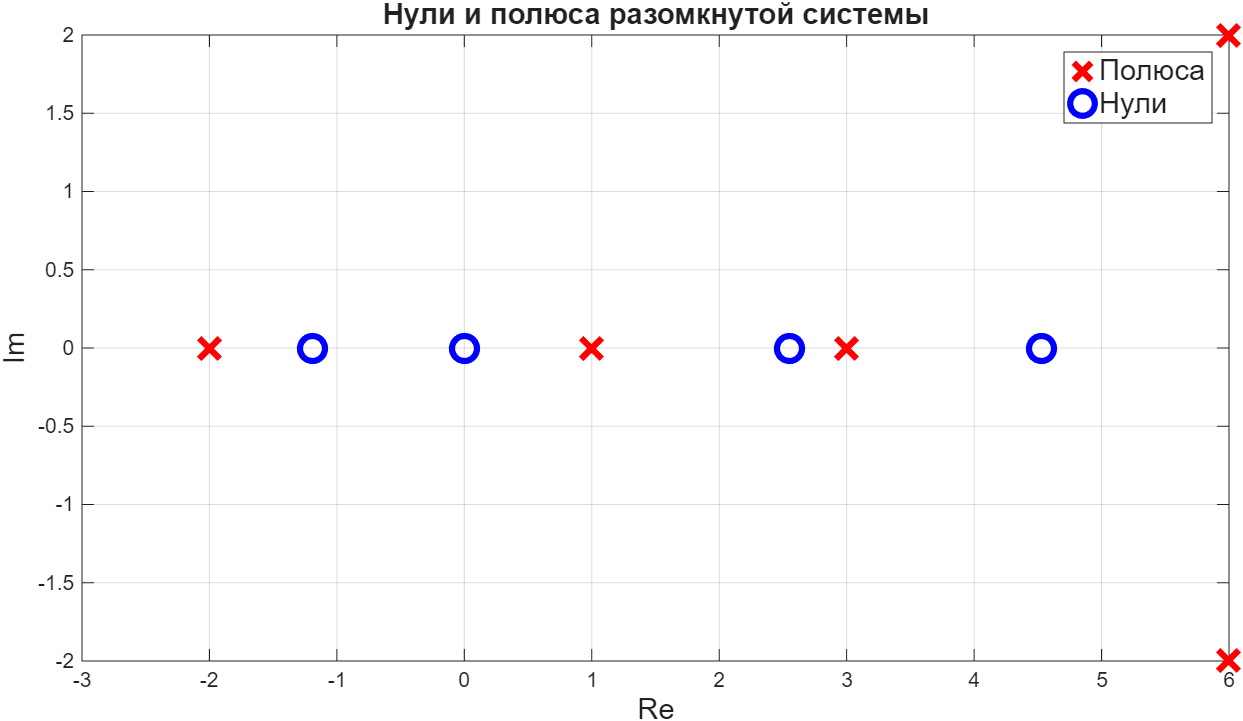
\includegraphics[width=0.75\linewidth]{images/Figure_6_1_1_1.png}
    \caption{Нули и полюса разомкнутой системы (1 объект)}
    \label{fig:placeholder}
\end{figure}

\begin{figure}[H]
    \centering
    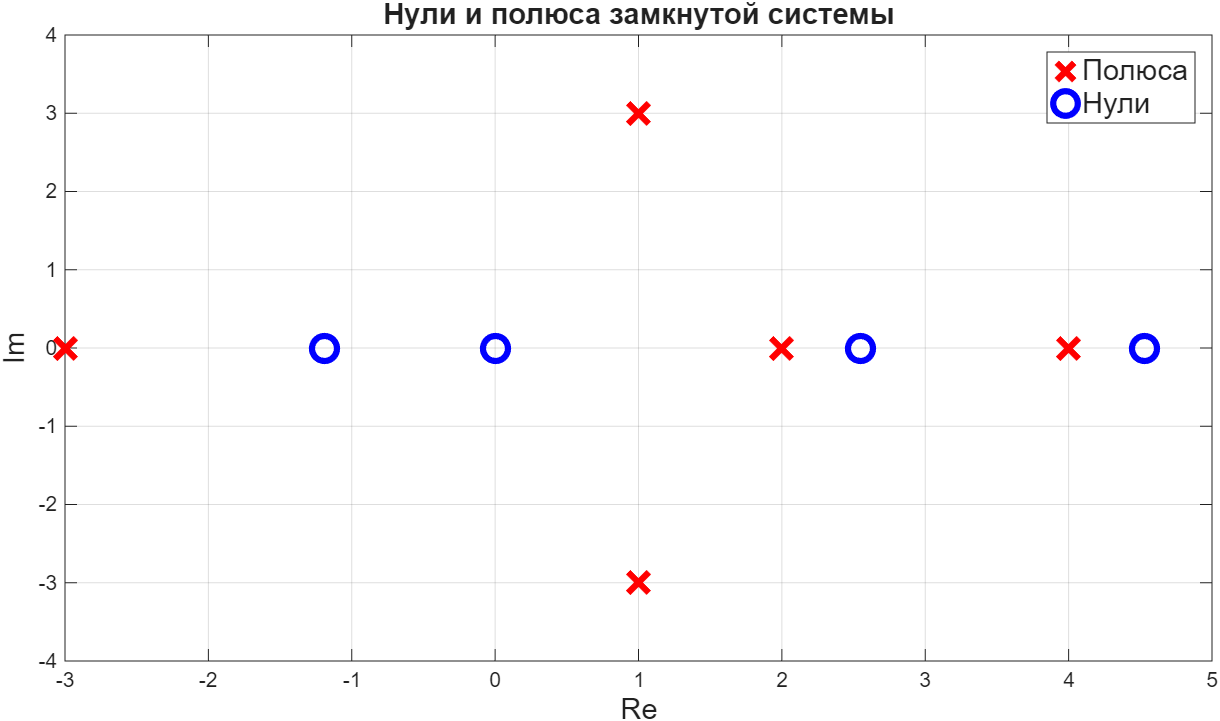
\includegraphics[width=0.75\linewidth]{images/Figure_6_1_1_2.png}
    \caption{Нули и полюса замкнутой системы (1 объект)}
    \label{fig:placeholder}
\end{figure}

\begin{figure}[H]
    \centering
    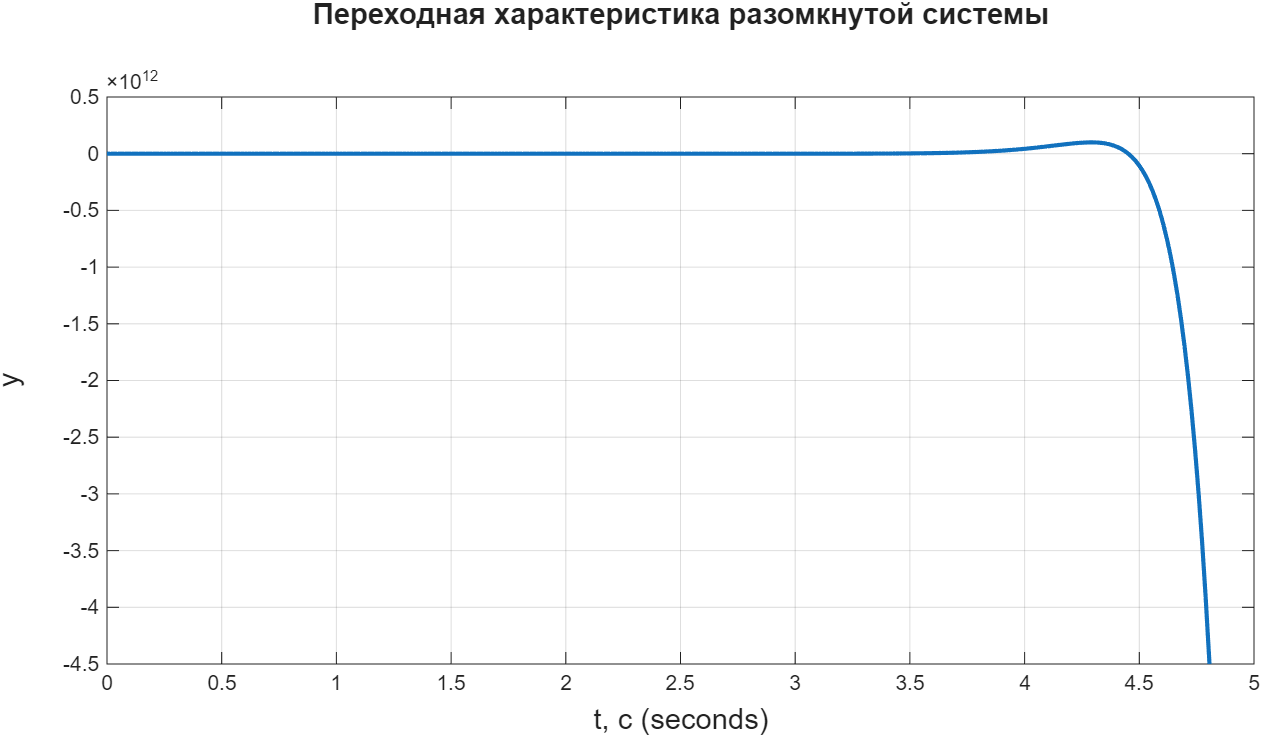
\includegraphics[width=0.75\linewidth]{images/Figure_6_1_1_3.png}
    \caption{Переходная характеристика разомкнутой системы (объект 1)}
    \label{fig:placeholder}
\end{figure}

\begin{figure}[H]
    \centering
    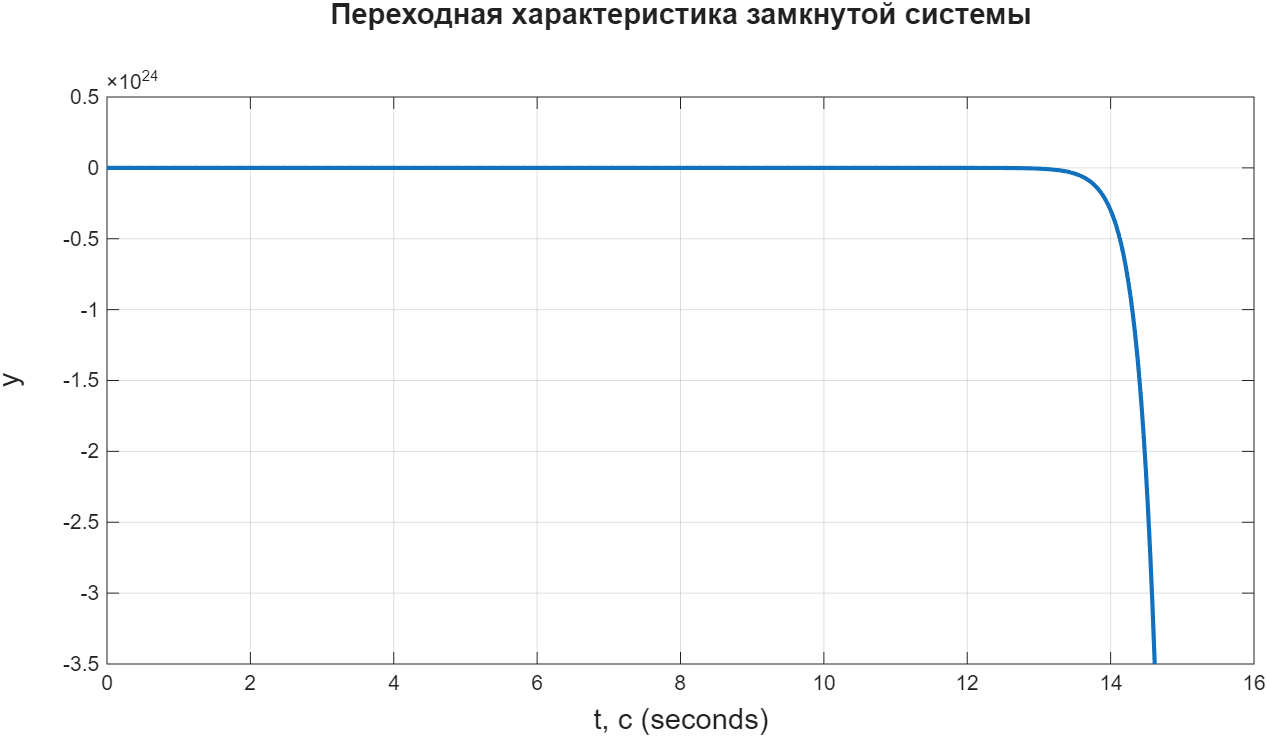
\includegraphics[width=0.75\linewidth]{images/Figure_6_1_1_4.png}
    \caption{Переходная характеристика замкнутой системы (объект 1)}
    \label{fig:placeholder}
\end{figure}

\begin{figure}[H]
    \centering
    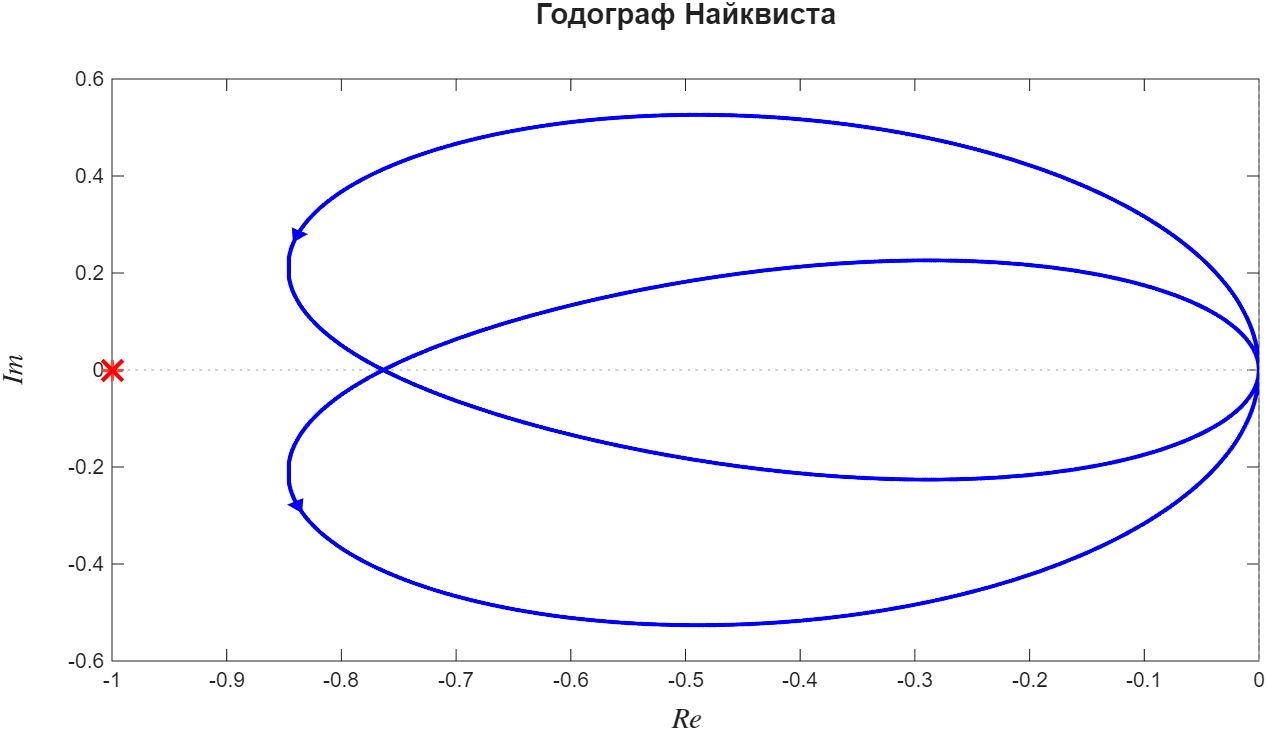
\includegraphics[width=0.75\linewidth]{images/Figure_6_1_1_5.png}
    \caption{Годограф Найквиста первого объекта}
    \label{fig:placeholder}
\end{figure}

Годограф Найквиста должен был совершить 0 оборотов вокруг точки $(-1, 0)$ по часовой стрелке. Как мы видим по графику теория совпала с практикой. 

\begin{figure}[H]
    \centering
    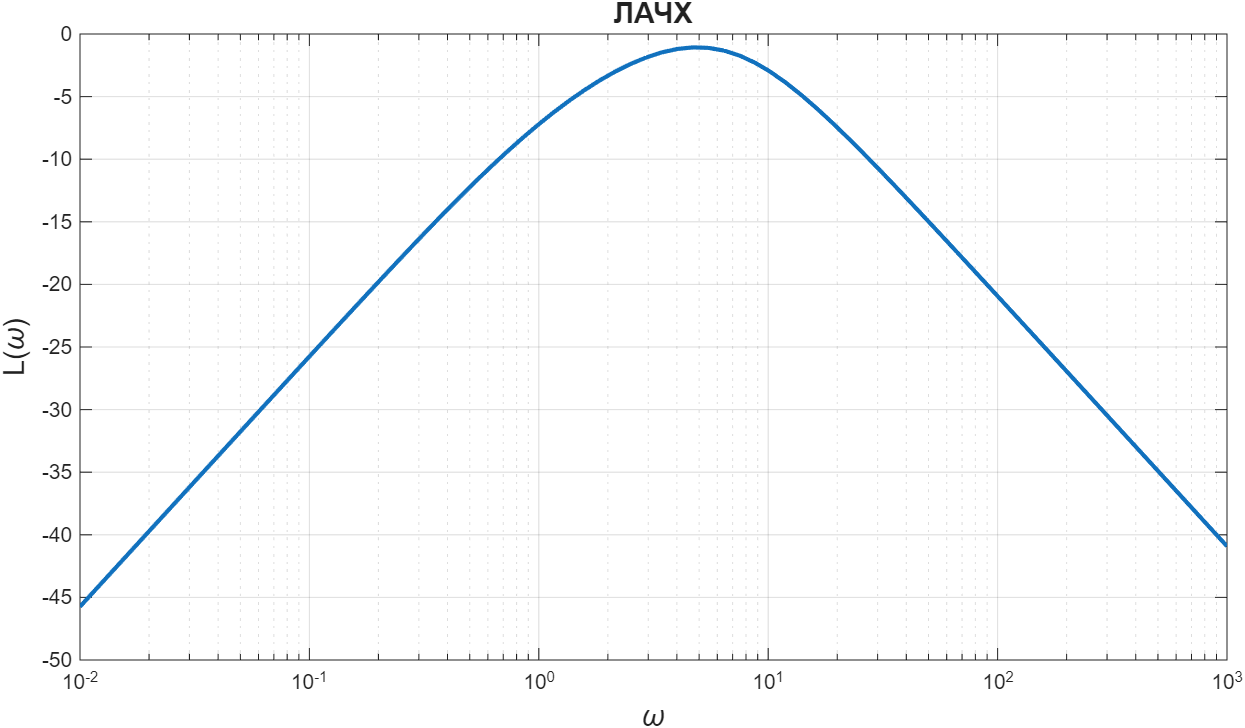
\includegraphics[width=0.75\linewidth]{images/Figure_6_1_1_6.png}
    \caption{ЛАЧХ первого объекта}
    \label{fig:placeholder}
\end{figure}

\begin{figure}[H]
    \centering
    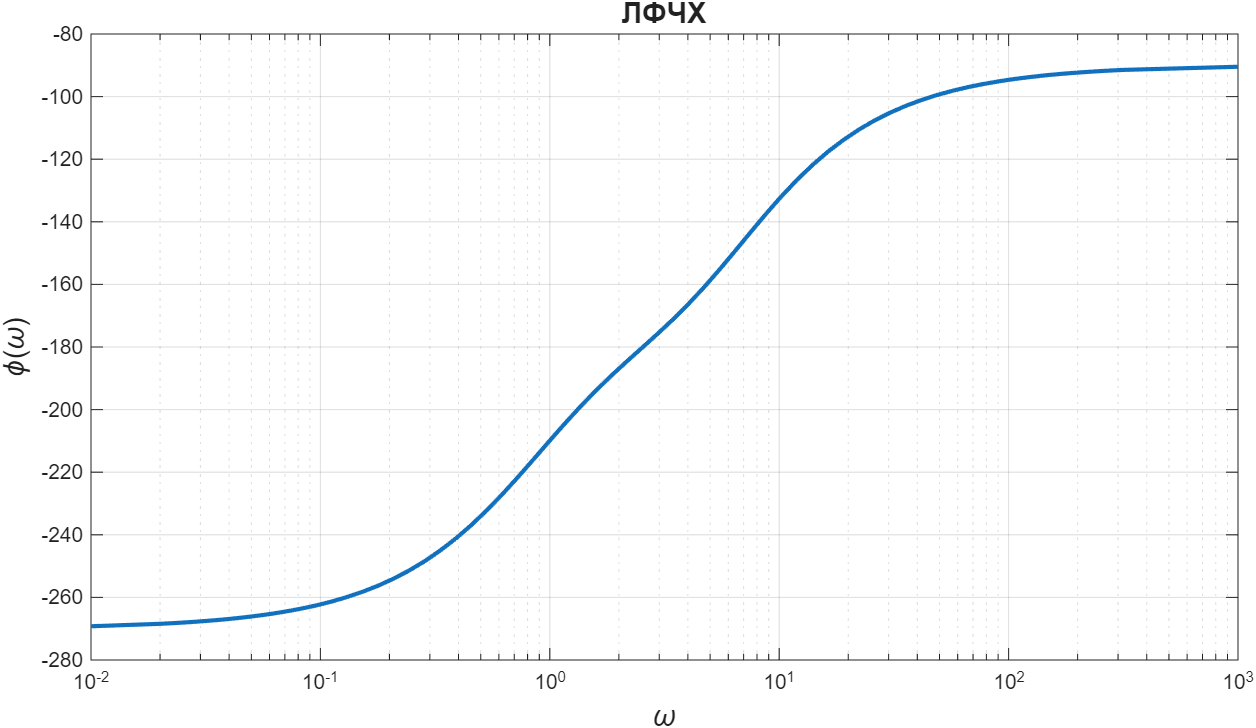
\includegraphics[width=0.75\linewidth]{images/Figure_6_1_1_7.png}
    \caption{ЛФЧХ первого объекта}
    \label{fig:placeholder}
\end{figure}

Как мы видим по графику ЛАЧХ $L(\omega)<0$ при любой частоте, следовательно, мы имеем $N=0$ переходов ЛФЧХ через критические уровни с положительной амплитудой.

По логарифмическому критерию Найквиста: для того, чтобы замкнутая система была устойчивой, необходимо и достаточно, чтобы разность между положительными и отрицательными переходами ЛФЧХ при частотах, когда $L(\omega)>0$, была равна $\frac{n}{2}$.

$$
\dfrac{n}{2}=2\neq 0
$$

Следовательно система неустойчива по логарифмическому критерию Найквиста.

Также по критерию Найквиста $N=n-m$. Мы знаем, что $N=0$ а $n=4$, тогда $m=n-2\cdot N=4$, что сходится с начальными условиями.


\subsection{Объект 2 (n=0, m=4)}

Полюса для разомкнутой системы:
$$
s_1= -1,\quad s_2=-2 ,\quad s_3=-3 ,\quad s_4=-6+j ,\quad s_5=-6-j
$$

Полюса для замкнутой системы:
$$
s_{\text{з}1}=3 ,\quad s_{\text{з}2}=2 ,\quad s_{\text{з}3}=-4 ,\quad s_{\text{з}4}=1+2j ,\quad s_{\text{з}5}=1-2j
$$

Характеристические уравнения примут вид:

$$
Q(s) = (s+1)(s+2)(s+3)(s+6-j)(s+6+j) = s^5 + 18s^4 + 120s^3 + 360s^2 + 479s + 222
$$

$$
D(s) = (s-3)(s-2)(s+4)(s-1-2j)(s-1+2j) = s^5 - 3s^4 - 7s^3 + 47s^2 - 118s + 120
$$

Числитель передаточной функции будет равен:

$$
R(s) = D(s) - Q(s) = -21s^4 - 127s^3 - 313s^2 - 597s -102
$$

По критерию Найквиста число оборотов годографа по часовой стрелке вокруг точки $(-1, 0)$ должно равняться:

$$
m-n=4-0=4
$$

\begin{figure}[H]
    \centering
    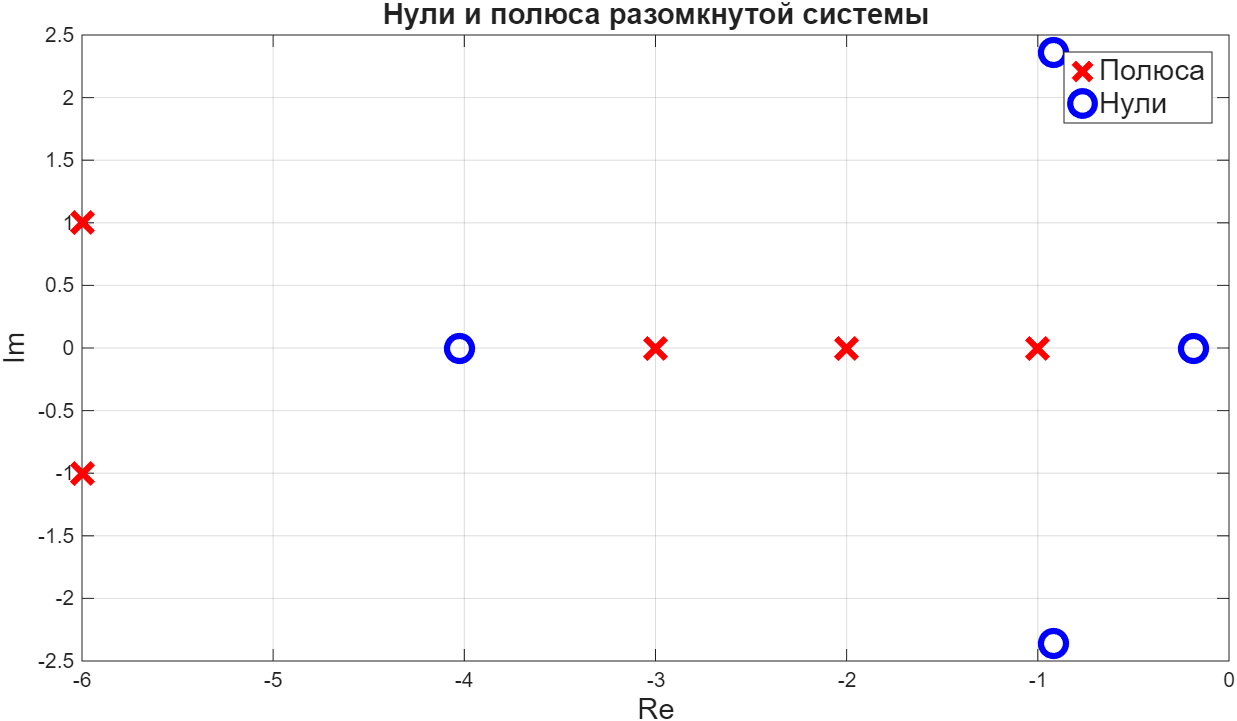
\includegraphics[width=0.75\linewidth]{images/Figure_6_1_2_1.png}
    \caption{Нули и полюса разомкнутой системы (2 объект)}
    \label{fig:placeholder}
\end{figure}

\begin{figure}[H]
    \centering
    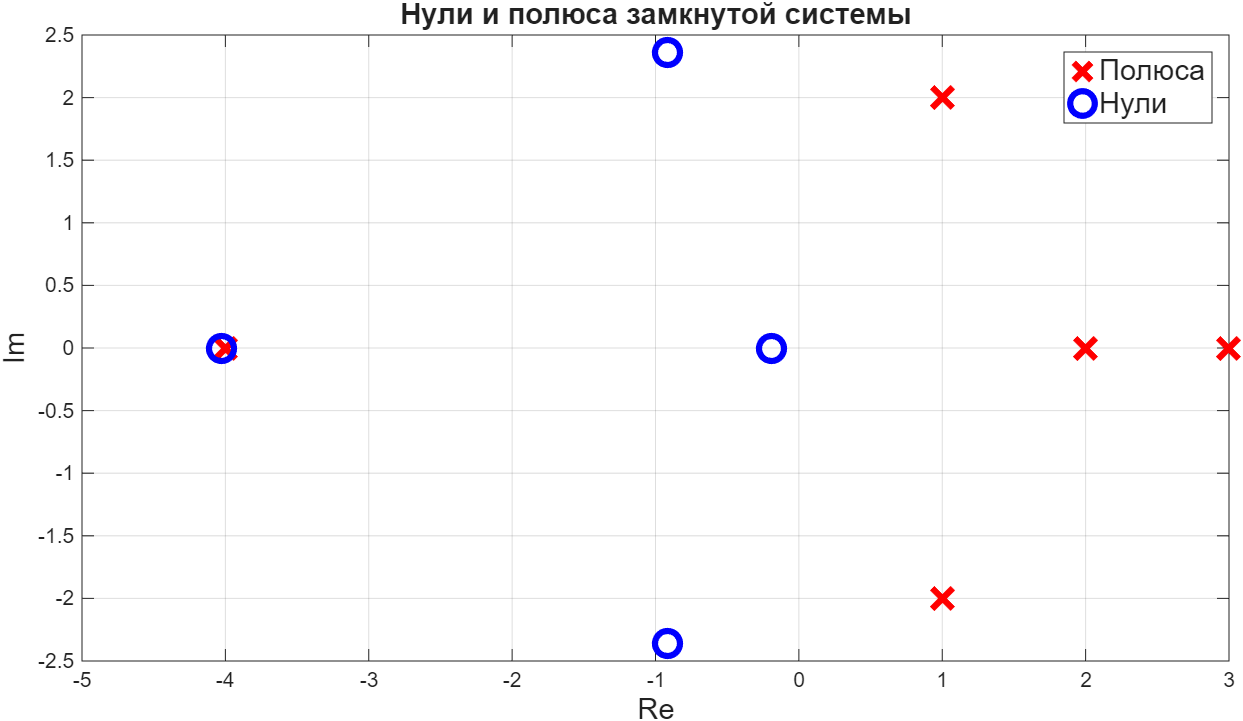
\includegraphics[width=0.75\linewidth]{images/Figure_6_1_2_2.png}
    \caption{Нули и полюса замкнутой системы (2 объект)}
    \label{fig:placeholder}
\end{figure}

\begin{figure}[H]
    \centering
    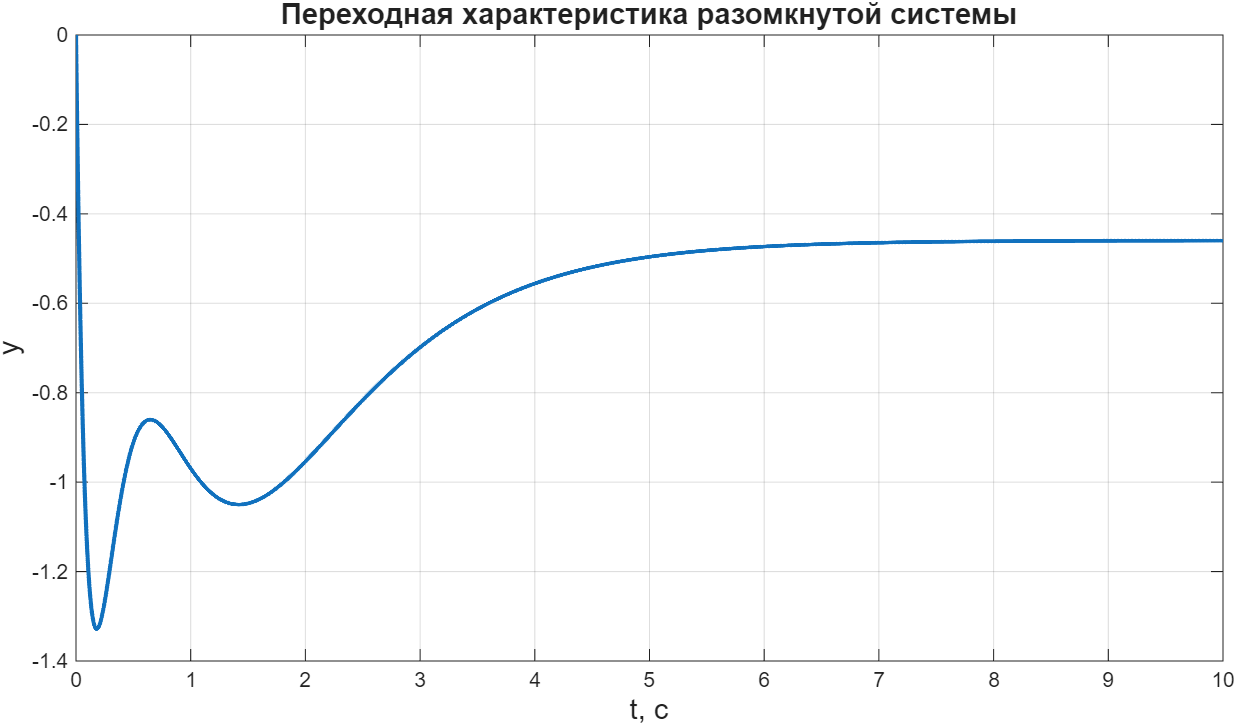
\includegraphics[width=0.75\linewidth]{images/Figure_6_1_2_3.png}
    \caption{Переходная характеристика разомкнутой системы (объект 2)}
    \label{fig:placeholder}
\end{figure}

\begin{figure}[H]
    \centering
    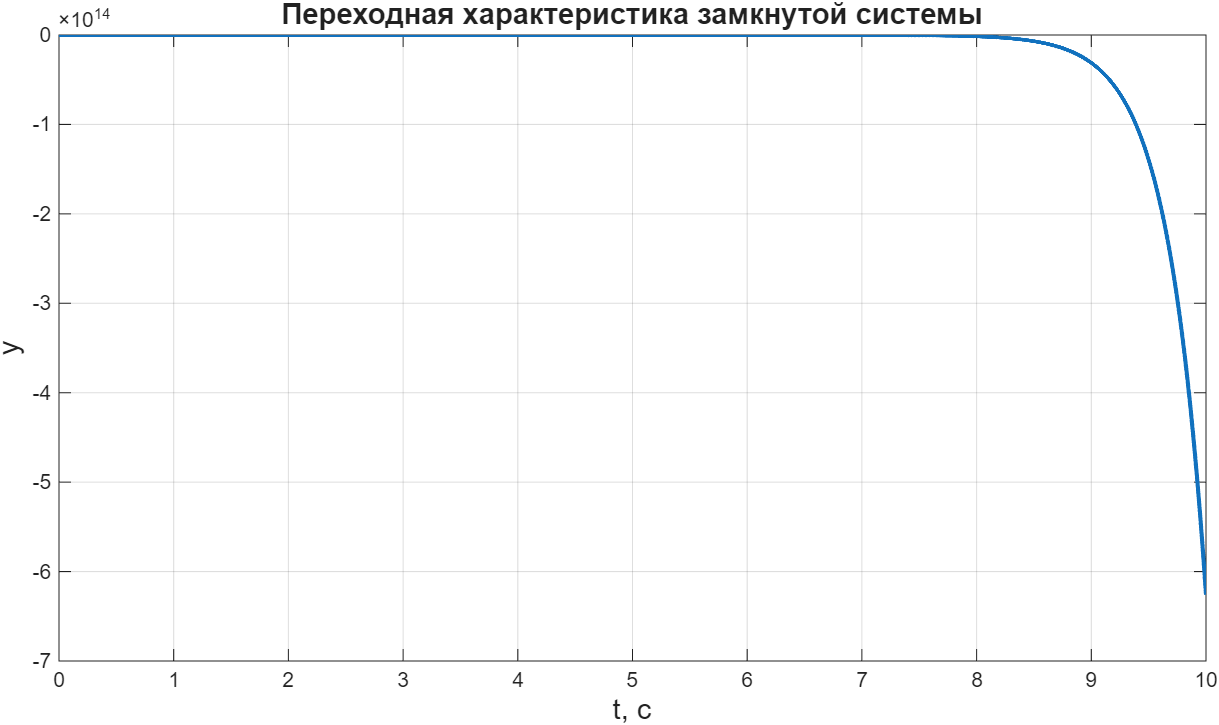
\includegraphics[width=0.75\linewidth]{images/Figure_6_1_2_4.png}
    \caption{Переходная характеристика замкнутой системы (объект 2)}
    \label{fig:placeholder}
\end{figure}

\begin{figure}[H]
    \centering
    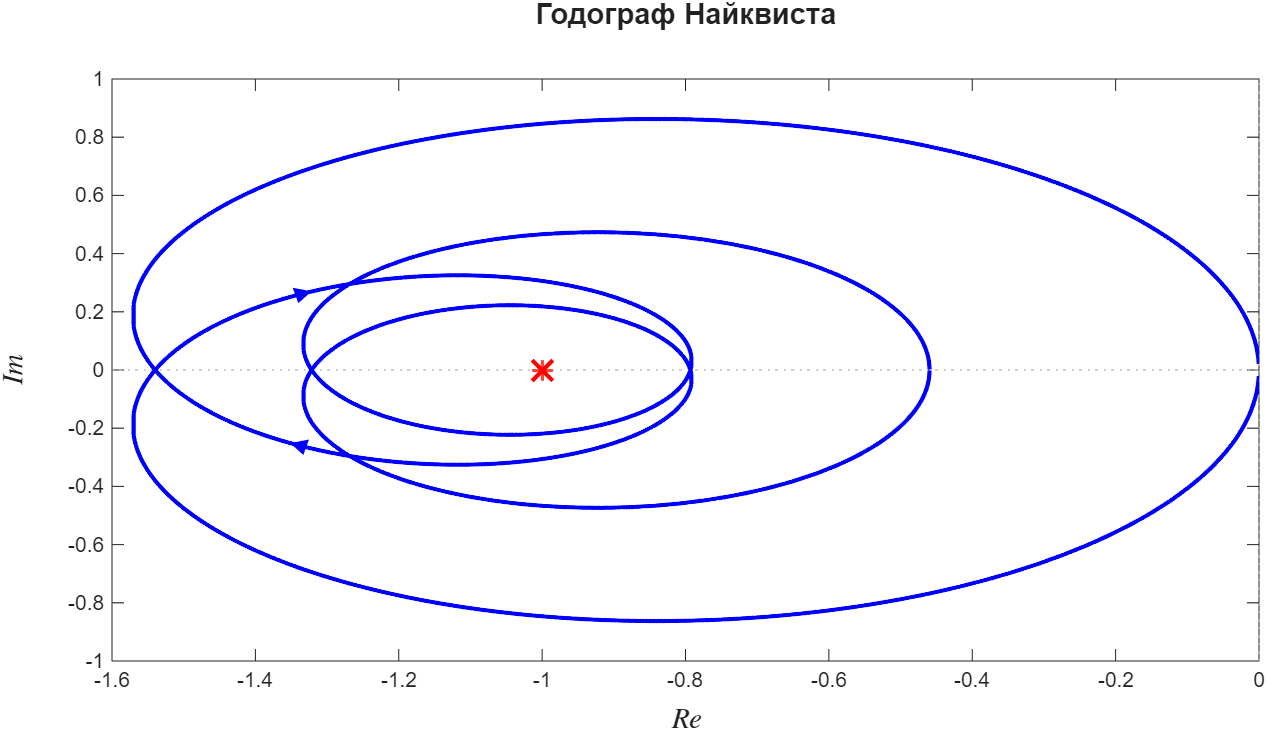
\includegraphics[width=0.75\linewidth]{images/Figure_6_1_2_5.png}
    \caption{Годограф Найквиста второго объекта}
    \label{fig:placeholder}
\end{figure}

Годограф Найквиста должен был совершить 4 оборотов вокруг точки $(-1, 0)$ по часовой стрелке. Как мы видим по графику теория совпала с практикой. 

\begin{figure}[H]
    \centering
    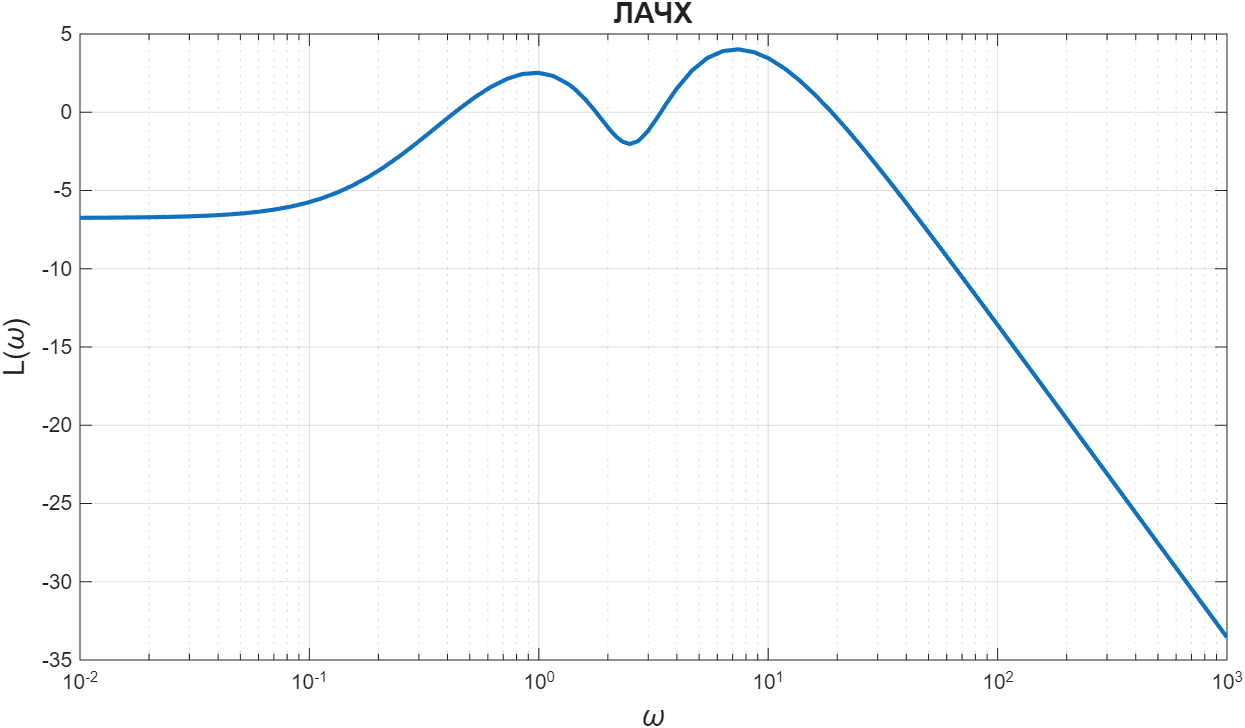
\includegraphics[width=0.75\linewidth]{images/Figure_6_1_2_6.png}
    \caption{ЛАЧХ второго объекта}
    \label{fig:placeholder}
\end{figure}

\begin{figure}[H]
    \centering
    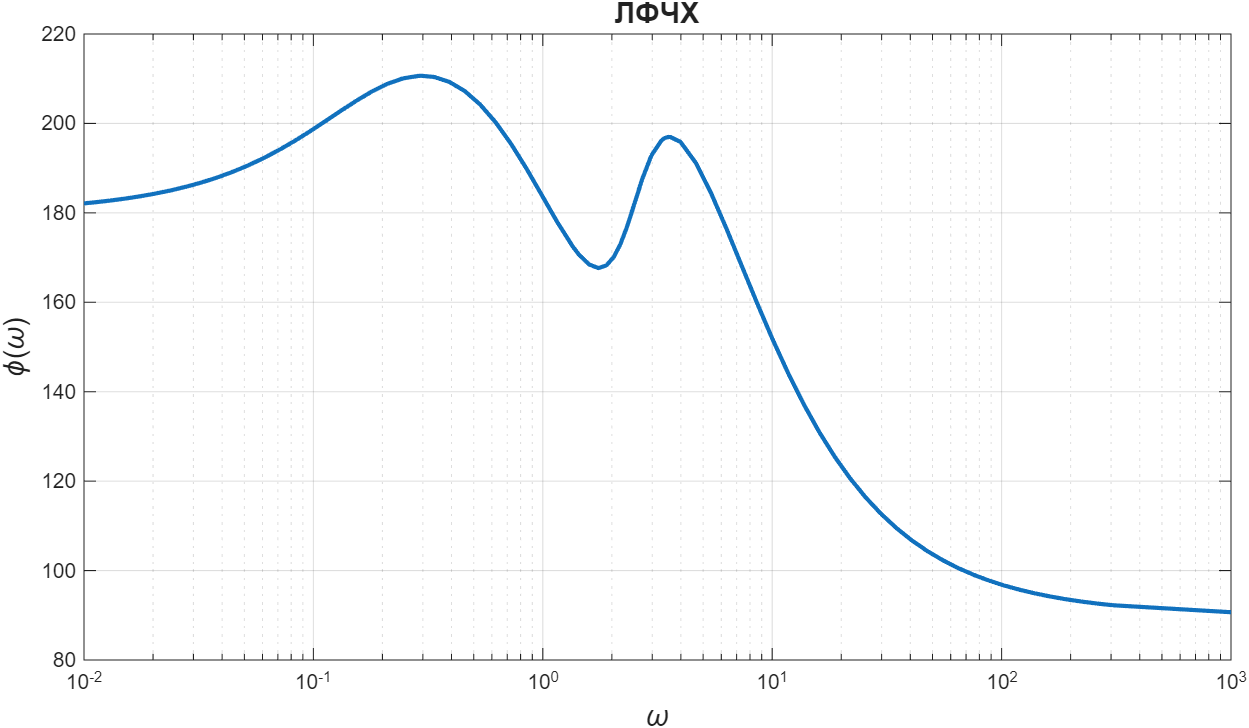
\includegraphics[width=0.75\linewidth]{images/Figure_6_1_2_7.png}
    \caption{ЛФЧХ второго объекта}
    \label{fig:placeholder}
\end{figure}

Как мы видим по графикам в области $L(\omega)>0$, ЛФЧХ имеет два отрицательных перехода, следовательно, мы имеем $N=-2$ переходов ЛФЧХ через критические уровни с положительной амплитудой.

По логарифмическому критерию Найквиста: для того, чтобы замкнутая система была устойчивой, необходимо и достаточно, чтобы разность между положительными и отрицательными переходами ЛФЧХ при частотах, когда $L(\omega)>0$, была равна $\frac{n}{2}$.

$$
\dfrac{n}{2}=0\neq -2
$$

Следовательно система неустойчива по логарифмическому критерию Найквиста.

Также по критерию Найквиста $N=n-m$. Мы знаем, что $N=-2$ а $n=0$, тогда $m=n-2 \cdot N=4$, что сходится с начальными условиями.


\subsection{Объект 3 (n=4, m=0)}

Полюса для разомкнутой системы:
$$
s_1= 1,\quad s_2=2 ,\quad s_3=-3 ,\quad s_4=3+j ,\quad s_5=3-j
$$

Полюса для замкнутой системы:
$$
s_{\text{з}1}=-1 ,\quad s_{\text{з}2}=-2 ,\quad s_{\text{з}3}=-4 ,\quad s_{\text{з}4}=-5+2j ,\quad s_{\text{з}5}=-5-2j
$$

Характеристические уравнения примут вид:

$$
Q(s) = (s-1)(s-2)(s+3)(s-3-j)(s-3+j) = s^5 -6s^4 + 3s^3 +48s^2 -106s +60
$$

$$
D(s) = (s+1)(s+2)(s+4)(s+5-2j)(s+5+2j) = s^5 +17s^4 +113s^3 + 351s^2 + 486s +232
$$

Числитель передаточной функции будет равен:

$$
R(s) = D(s) - Q(s) = 23s^4 + 110s^3 + 303s^2 + 592s + 172 
$$

По критерию Найквиста число оборотов годографа по часовой стрелке вокруг точки $(-1, 0)$ должно равняться:

$$
m-n=0-4=-4
$$

\begin{figure}[H]
    \centering
    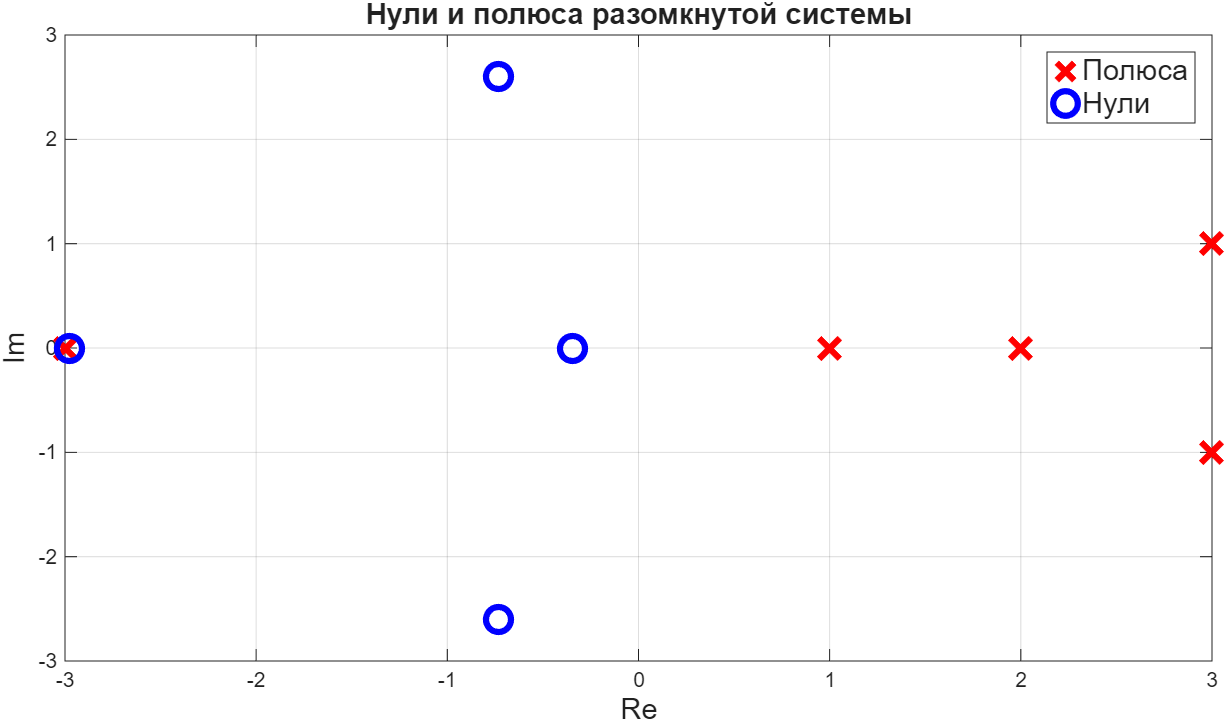
\includegraphics[width=0.75\linewidth]{images/Figure_6_1_3_1.png}
    \caption{Нули и полюса разомкнутой системы (3 объект)}
    \label{fig:placeholder}
\end{figure}

\begin{figure}[H]
    \centering
    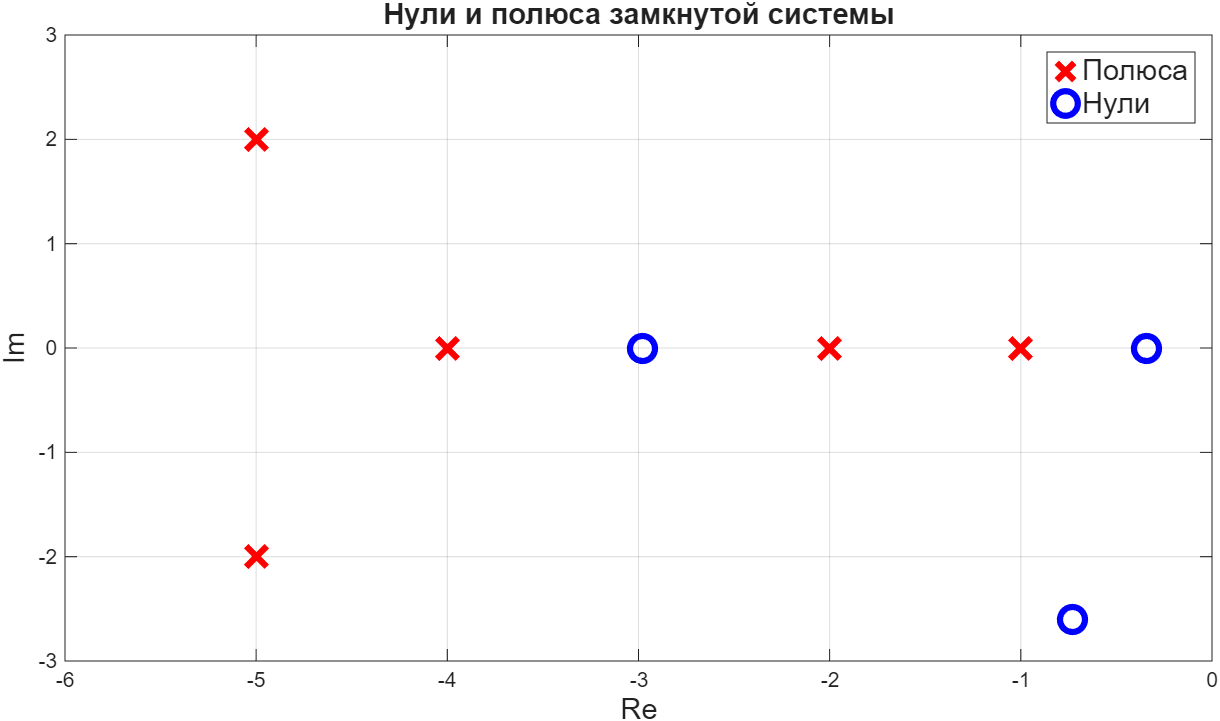
\includegraphics[width=0.75\linewidth]{images/Figure_6_1_3_2.png}
    \caption{Нули и полюса замкнутой системы (3 объект)}
    \label{fig:placeholder}
\end{figure}

\begin{figure}[H]
    \centering
    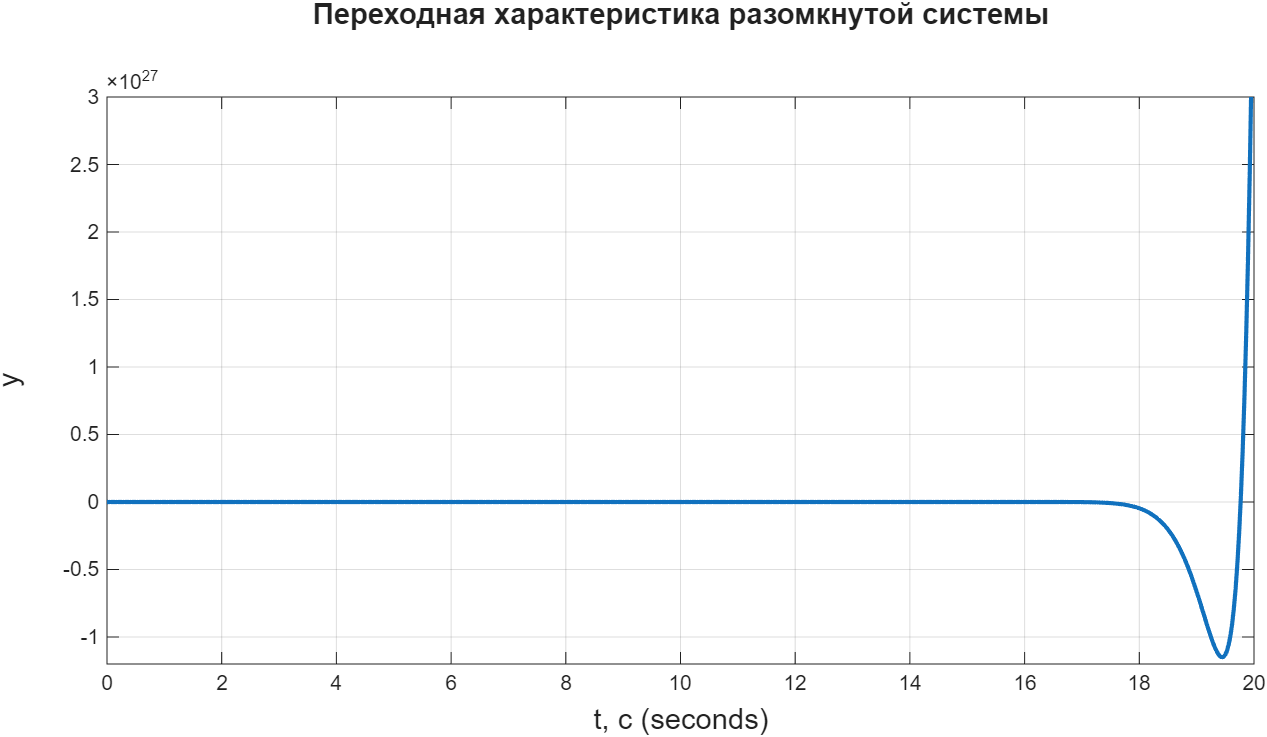
\includegraphics[width=0.75\linewidth]{images/Figure_6_1_3_3.png}
    \caption{Переходная характеристика разомкнутой системы (объект 3)}
    \label{fig:placeholder}
\end{figure}

\begin{figure}[H]
    \centering
    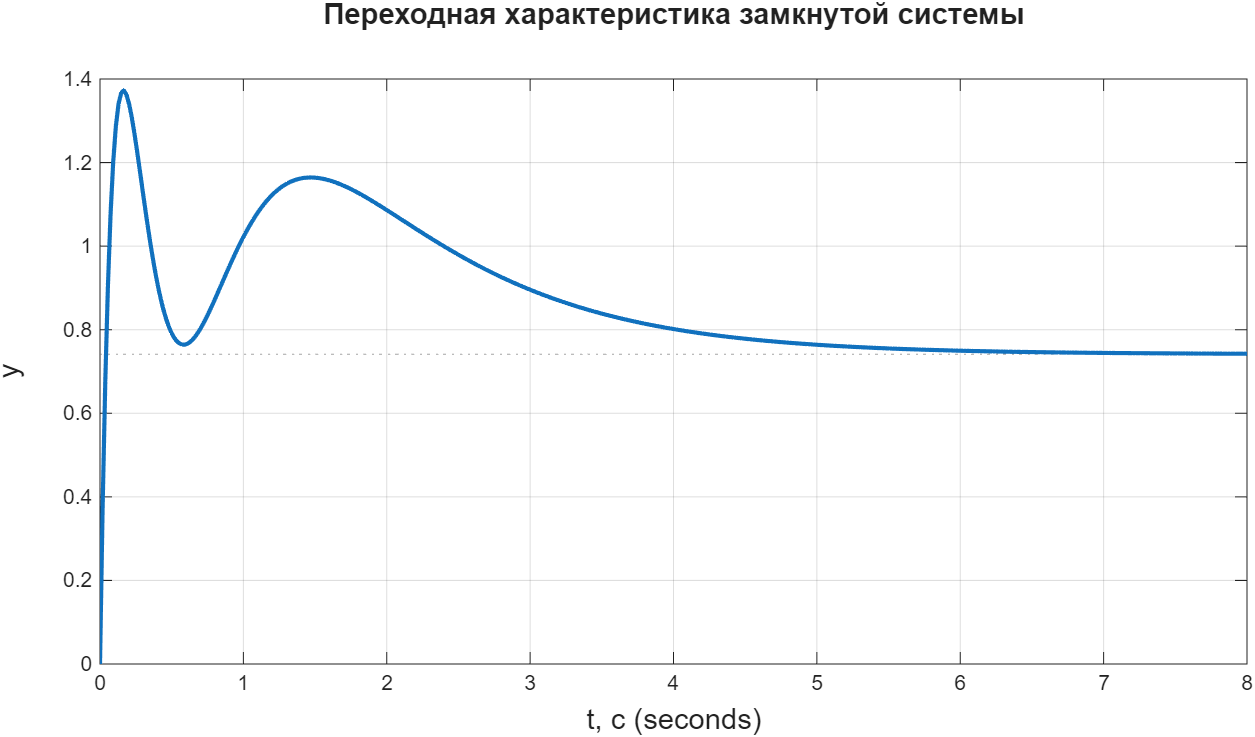
\includegraphics[width=0.75\linewidth]{images/Figure_6_1_3_4.png}
    \caption{Переходная характеристика замкнутой системы (объект 3)}
    \label{fig:placeholder}
\end{figure}

\begin{figure}[H]
    \centering
    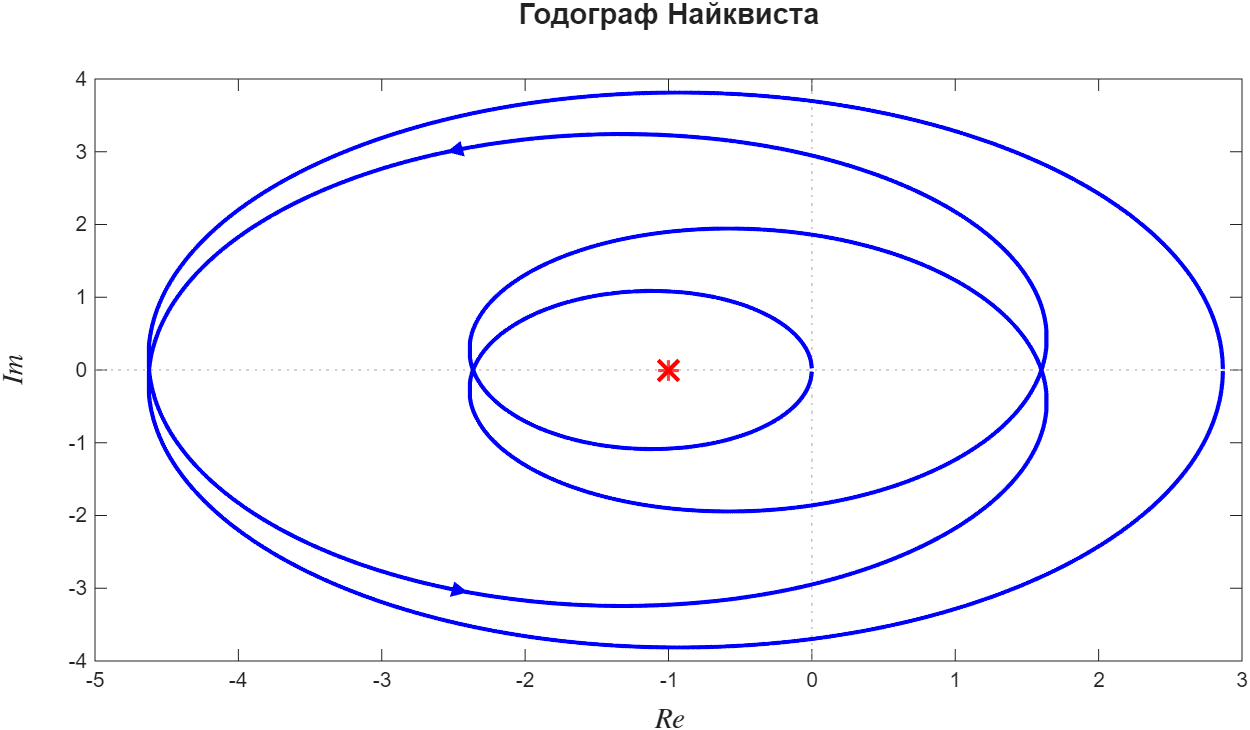
\includegraphics[width=0.75\linewidth]{images/Figure_6_1_3_5.png}
    \caption{Годограф Найквиста третьего объекта}
    \label{fig:placeholder}
\end{figure}

Годограф Найквиста должен был совершить 4 оборотов вокруг точки $(-1, 0)$ против часовой стрелки. Как мы видим по графику теория совпала с практикой. 

\begin{figure}[H]
    \centering
    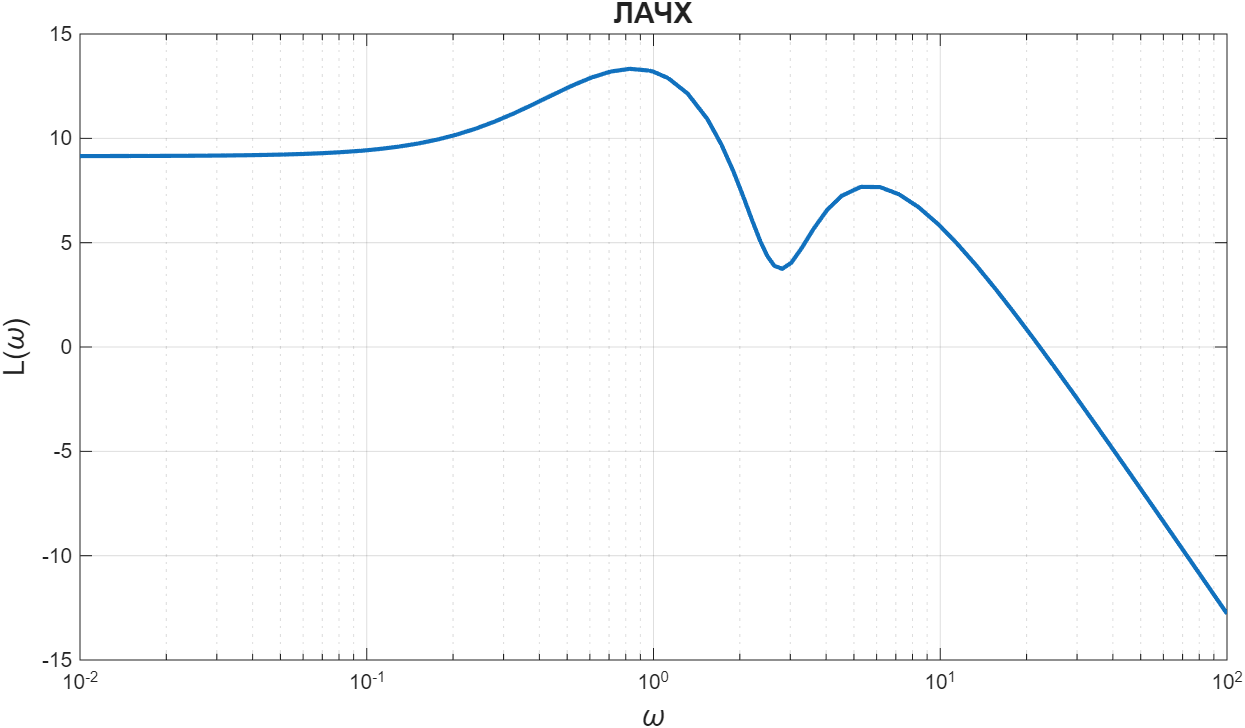
\includegraphics[width=0.75\linewidth]{images/Figure_6_1_3_6.png}
    \caption{ЛАЧХ третьего объекта}
    \label{fig:placeholder}
\end{figure}

\begin{figure}[H]
    \centering
    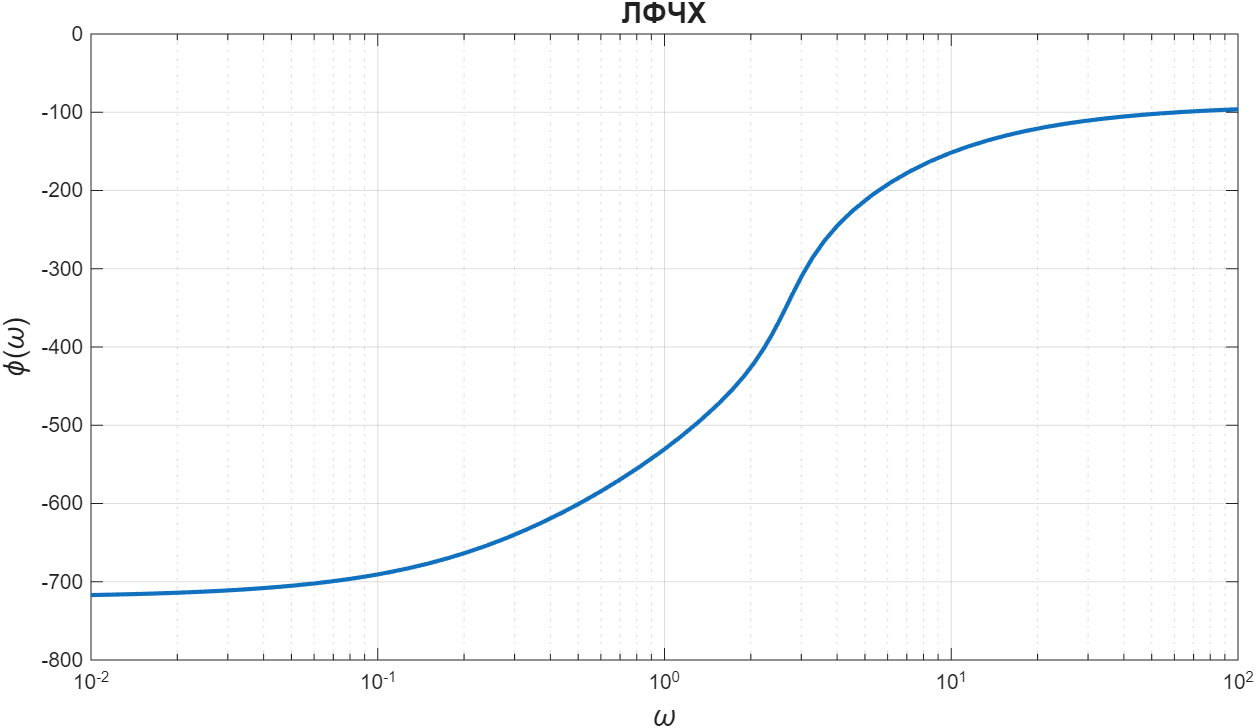
\includegraphics[width=0.75\linewidth]{images/Figure_6_1_3_7.png}
    \caption{ЛФЧХ третьего объекта}
    \label{fig:placeholder}
\end{figure}

Как мы видим по графикам в области $L(\omega)>0$, ЛФЧХ имеет два положительных перехода, следовательно, мы имеем $N=2$ переходов ЛФЧХ через критические уровни с положительной амплитудой.

По логарифмическому критерию Найквиста: для того, чтобы замкнутая система была устойчивой, необходимо и достаточно, чтобы разность между положительными и отрицательными переходами ЛФЧХ при частотах, когда $L(\omega)>0$, была равна $\frac{n}{2}$.

$$
\dfrac{4}{2}=2
$$

Следовательно система устойчива по логарифмическому критерию Найквиста.

Также по критерию Найквиста $N=n-m$. Мы знаем, что $N=2$ а $n=4$, тогда $m=n-2 \cdot N=0$, что сходится с начальными условиями.




\newpage

\section{Задание 2. Коэффициент усиления}

\subsection{Исходные данные:}
\begin{center}
\begin{tabular}{|c|c|}
\hline
     Параметр & Значение \\ \hline
     p&3\\ \hline
     q&2\\ \hline
     n&4\\ \hline
     m&4\\ \hline
     i&2\\ \hline
     j&6\\ \hline
\end{tabular}
\end{center}

\begin{center}
\begin{tabular}{|c|c|}
\hline
     $W_1(s)$ & $W_2(s)$ \\ \hline
     $\dfrac{s-2}{s^2+6s+5}$&$\dfrac{-9s^3+16s^2-6s}{10s^3+12s^2+5s+1}$\\ \hline
\end{tabular}
\end{center}

\subsection{Первая передаточная функция}

Домножим нашу передаточную функцию на коэффициент усисления $k$:

$$
W_1(s)=\dfrac{k(s-2)}{s^2+6s+5}
$$

Найдём корни характеристического уравнения разомкнутой системы $s^2+6s+5$:

\begin{figure}[H]
    \centering
    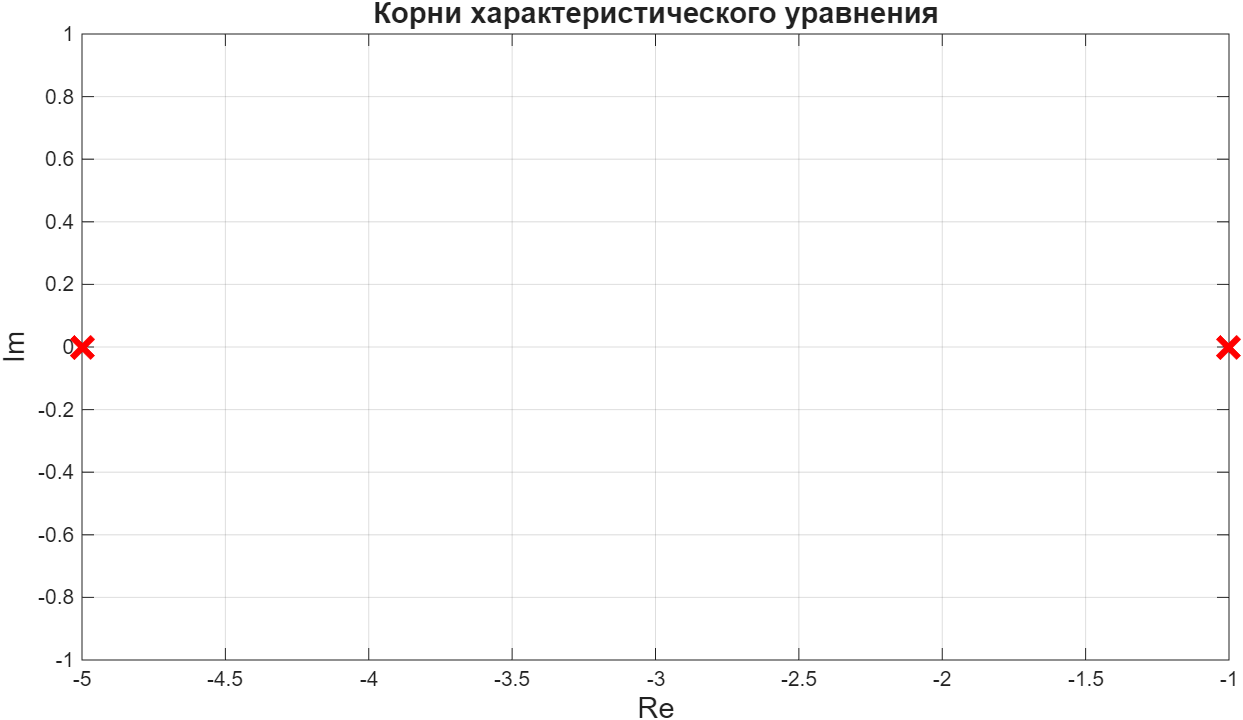
\includegraphics[width=0.75\linewidth]{images/Figure_6_2_1_1.png}
    \caption{Корни харатеристического уравнения разомкнутой системы}
    \label{fig:placeholder}
\end{figure}

Вещественная часть всех корней характеристического уравнения отрицательна $n=0$, следовательно для того чтобы замкнутая система стала неустойчивой годографу надо сделать хотябы один оборот по часовой стрелке вокруг точки (-1, 0).

Найдем передаточную функцию замкнутой системы:

$$
W_{\text{з}1}=\dfrac{\dfrac{k(s-2)}{s^2+6s+5}}{1+\dfrac{k(s-2)}{s^2+6s+5}}=\dfrac{k(s-2)}{s^2+s(6+k)+5-2k}
$$

\begin{figure}[H]
    \centering
    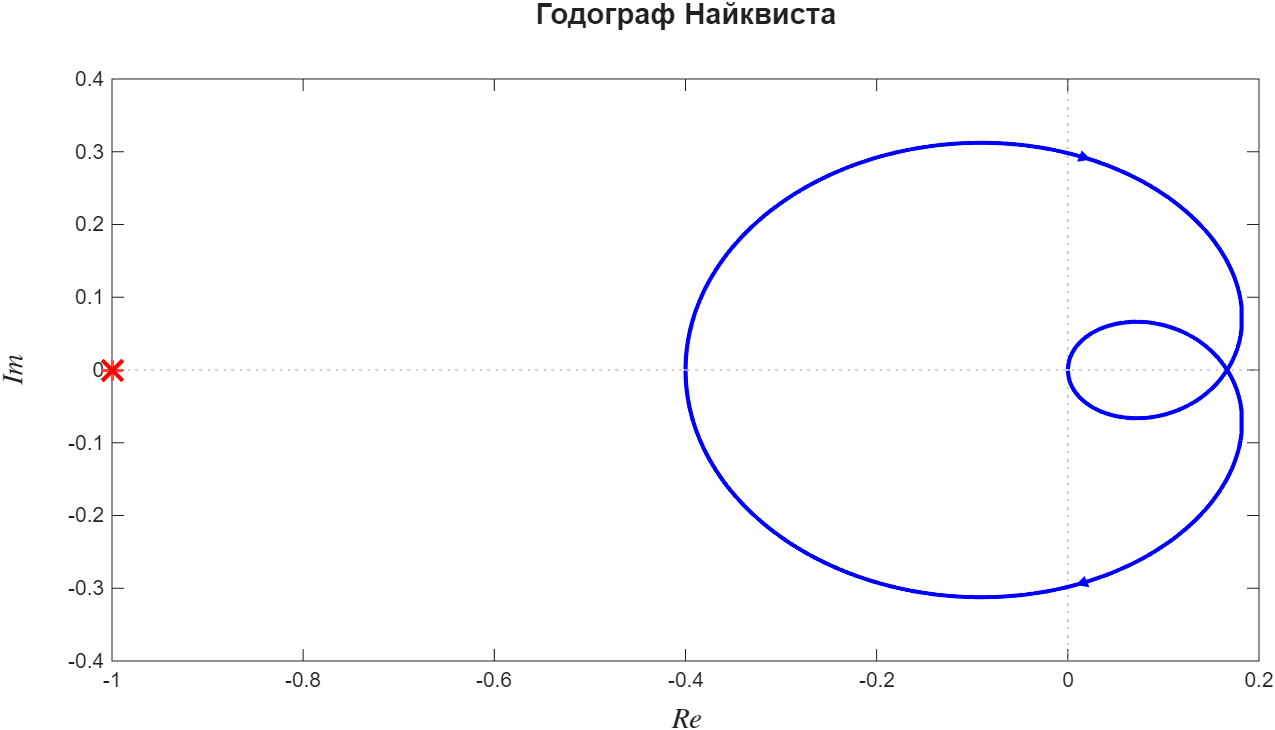
\includegraphics[width=0.75\linewidth]{images/Figure_6_2_1_2.png}
    \caption{Годограф Найквиста при $k=1$ (1 передаточная функция)}
    \label{fig:placeholder}
\end{figure}

По критерию Гурвинца система будет ассимптотически устойчива при:

$$
\begin{cases}
    1>0\\
    6+k>0\\
    5-2k>0
\end{cases}
$$

$$
\begin{cases}
    k>-6\\
    k<2.5
\end{cases}
$$

Так как по условию $k>0$ получаем промежуток при котором система будет ассимптотически устойчива:

$$
k\in (0,\ 2.5)
$$

Выберем разные $k$:

$$
k=\{1.5,\ 2,\ 3,\ 4\}
$$

\begin{figure}[H]
    \centering
    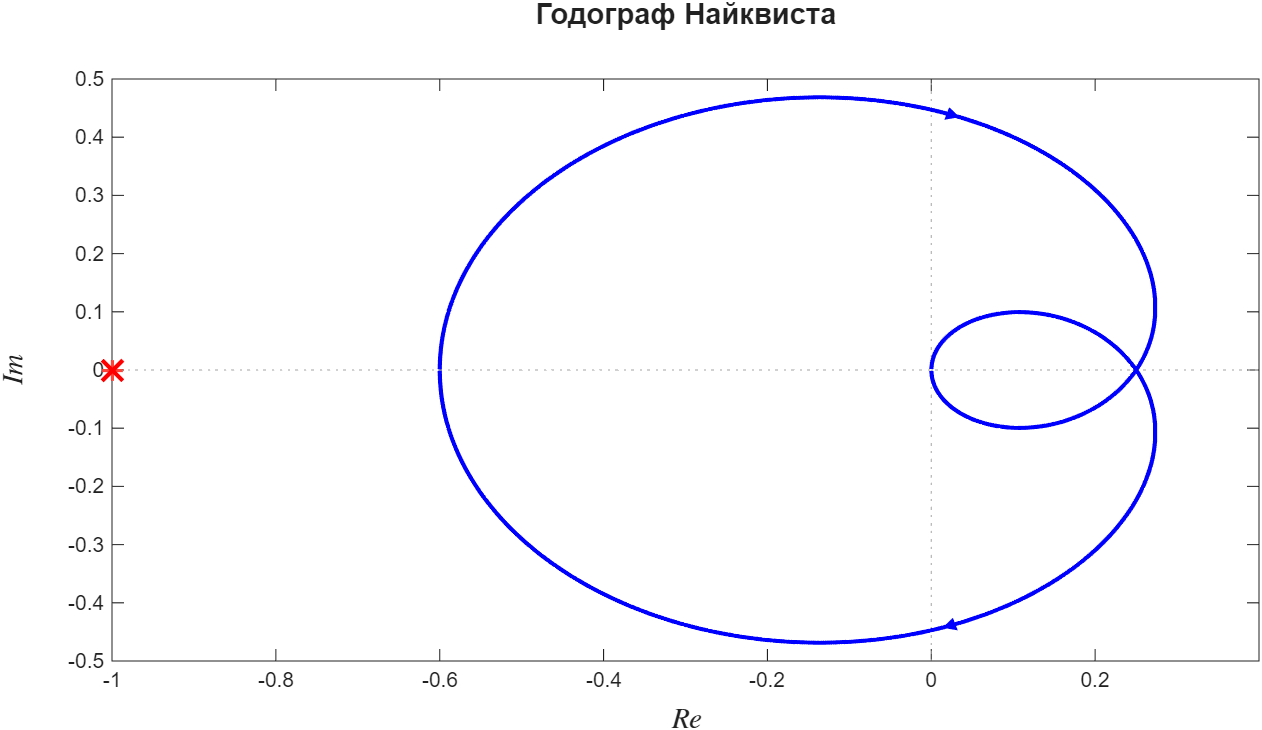
\includegraphics[width=0.75\linewidth]{images/Figure_6_2_1_3.png}
    \caption{Годограф Найквиста при $k=1.5$ (1 передаточная функция)}
    \label{fig:placeholder}
\end{figure}

\begin{figure}[H]
    \centering
    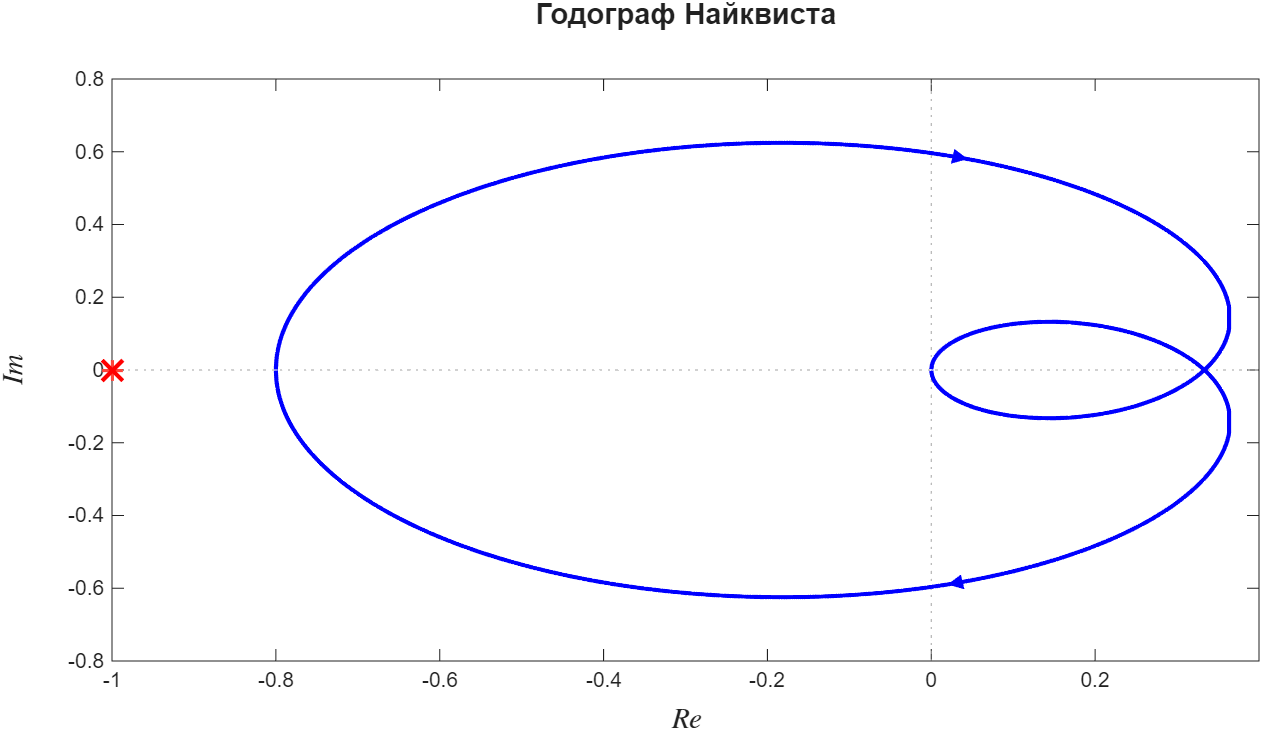
\includegraphics[width=0.75\linewidth]{images/Figure_6_2_1_4.png}
    \caption{Годограф Найквиста при $k=2$ (1 передаточная функция)}
    \label{fig:placeholder}
\end{figure}

\begin{figure}[H]
    \centering
    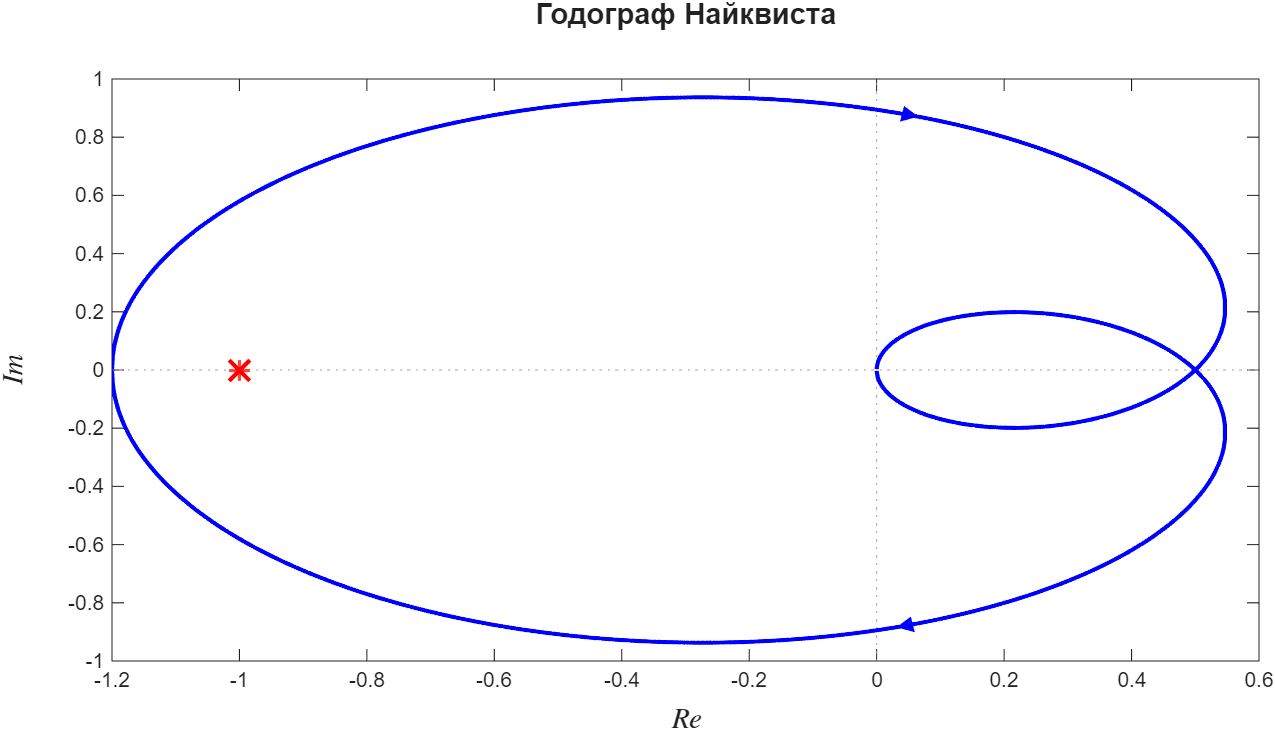
\includegraphics[width=0.75\linewidth]{images/Figure_6_2_1_5.png}
    \caption{Годограф Найквиста при $k=3$ (1 передаточная функция)}
    \label{fig:placeholder}
\end{figure}

\begin{figure}[H]
    \centering
    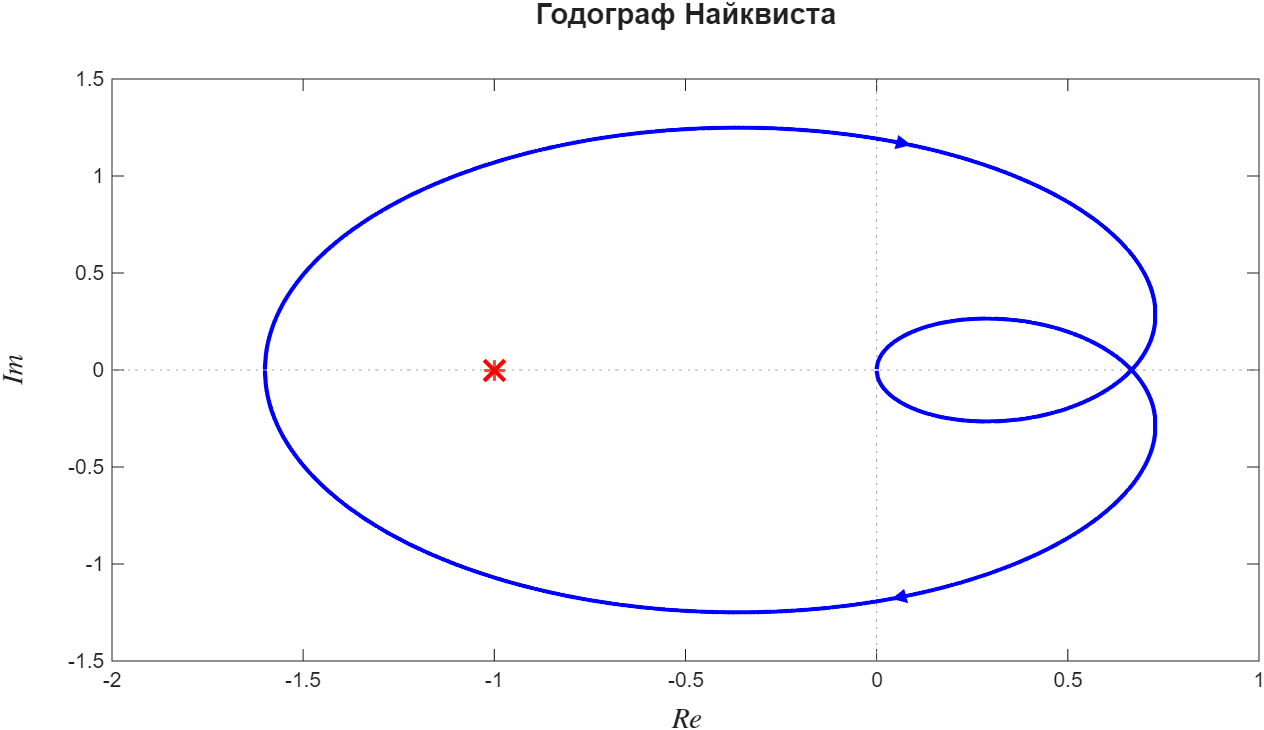
\includegraphics[width=0.75\linewidth]{images/Figure_6_2_1_6.png}
    \caption{Годограф Найквиста при $k=4$ (1 передаточная функция)}
    \label{fig:placeholder}
\end{figure}

\begin{figure}[H]
    \centering
    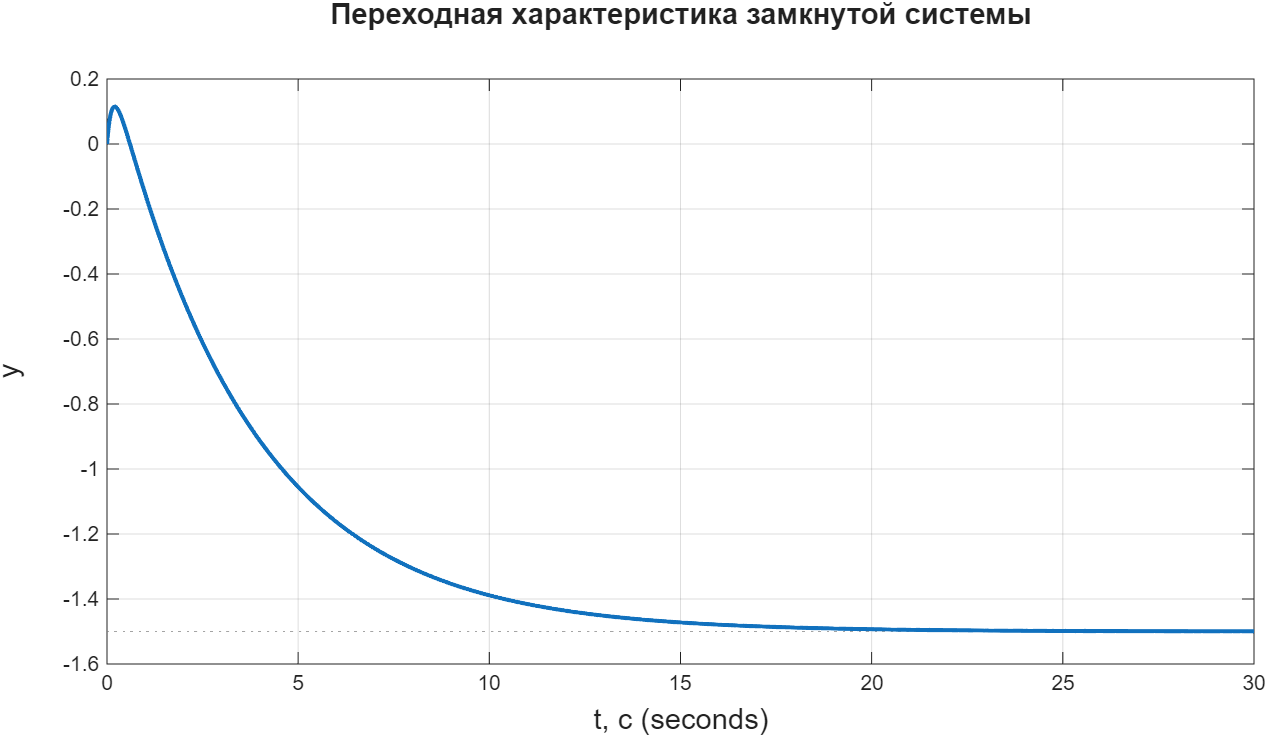
\includegraphics[width=0.75\linewidth]{images/Figure_6_2_1_7.png}
    \caption{Переходная характеристика при $k=1.5$ (1 передаточная функция)}
    \label{fig:placeholder}
\end{figure}

\begin{figure}[H]
    \centering
    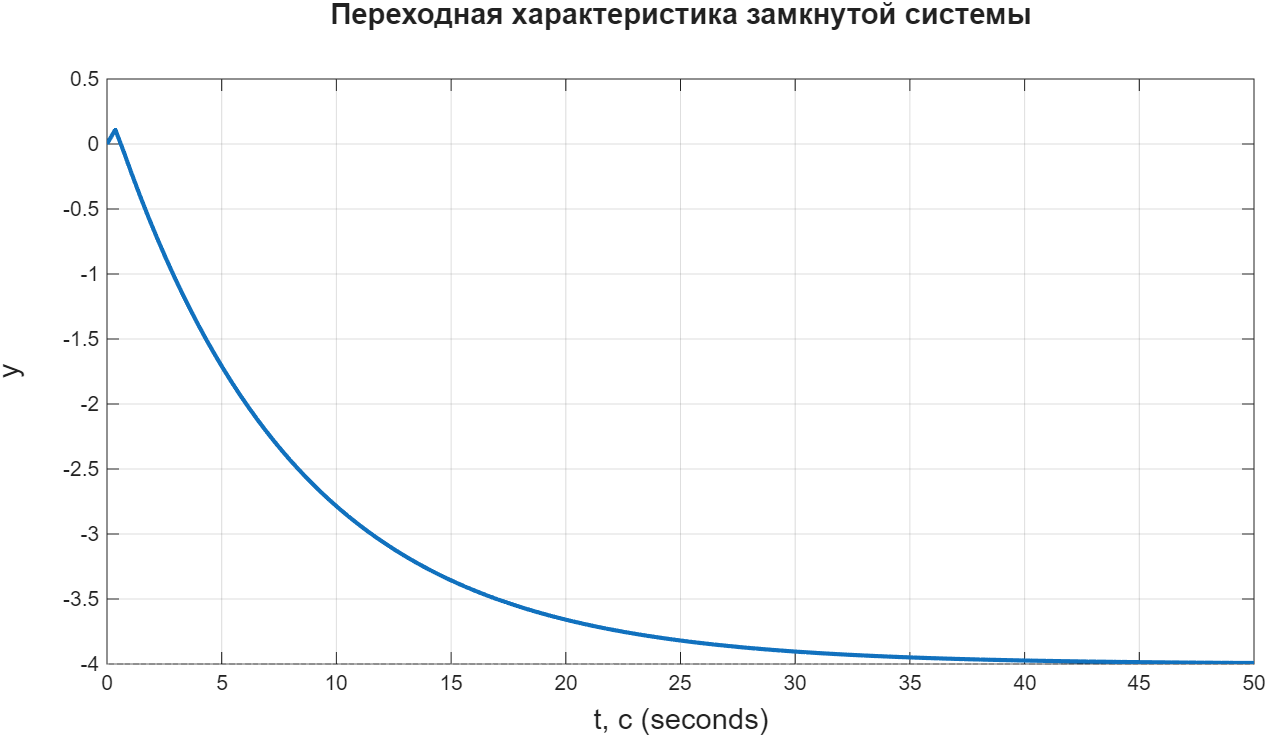
\includegraphics[width=0.75\linewidth]{images/Figure_6_2_1_8.png}
    \caption{Переходная характеристика при $k=2$ (1 передаточная функция)}
    \label{fig:placeholder}
\end{figure}

\begin{figure}[H]
    \centering
    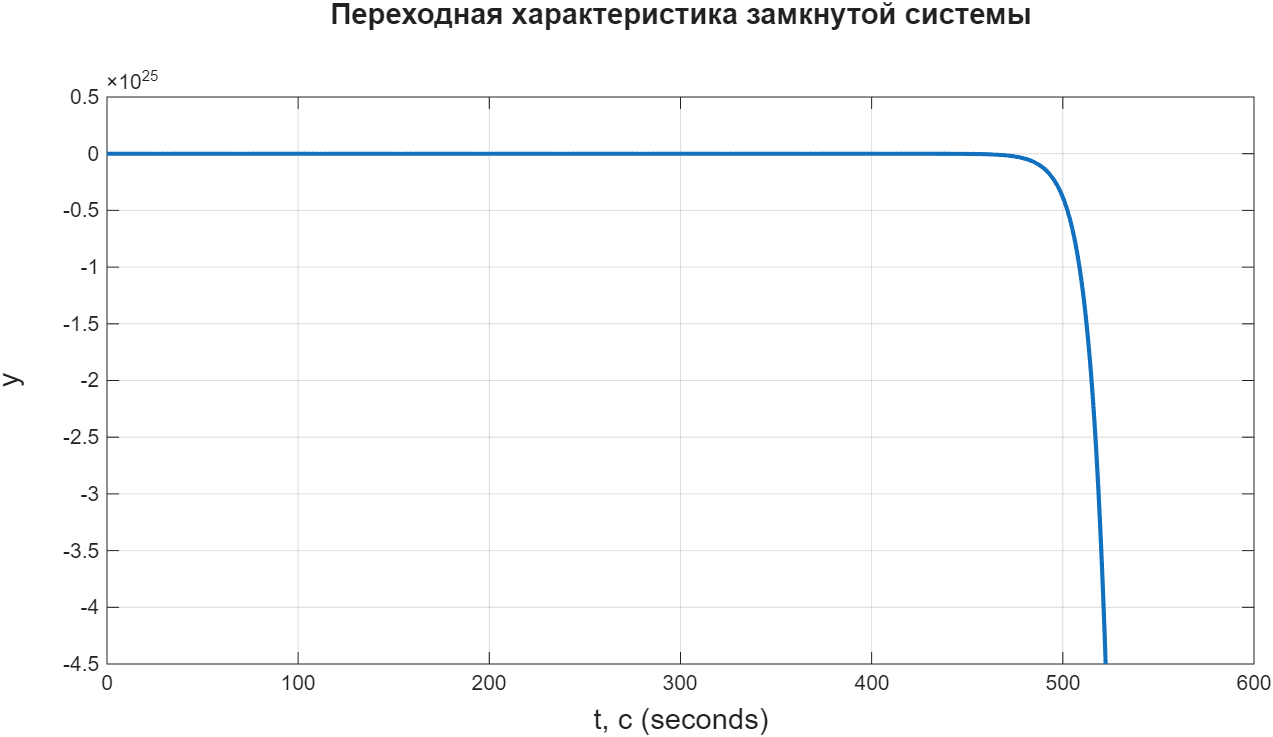
\includegraphics[width=0.75\linewidth]{images/Figure_6_2_1_9.png}
    \caption{Переходная характеристика при $k=3$ (1 передаточная функция)}
    \label{fig:placeholder}
\end{figure}

\begin{figure}[H]
    \centering
    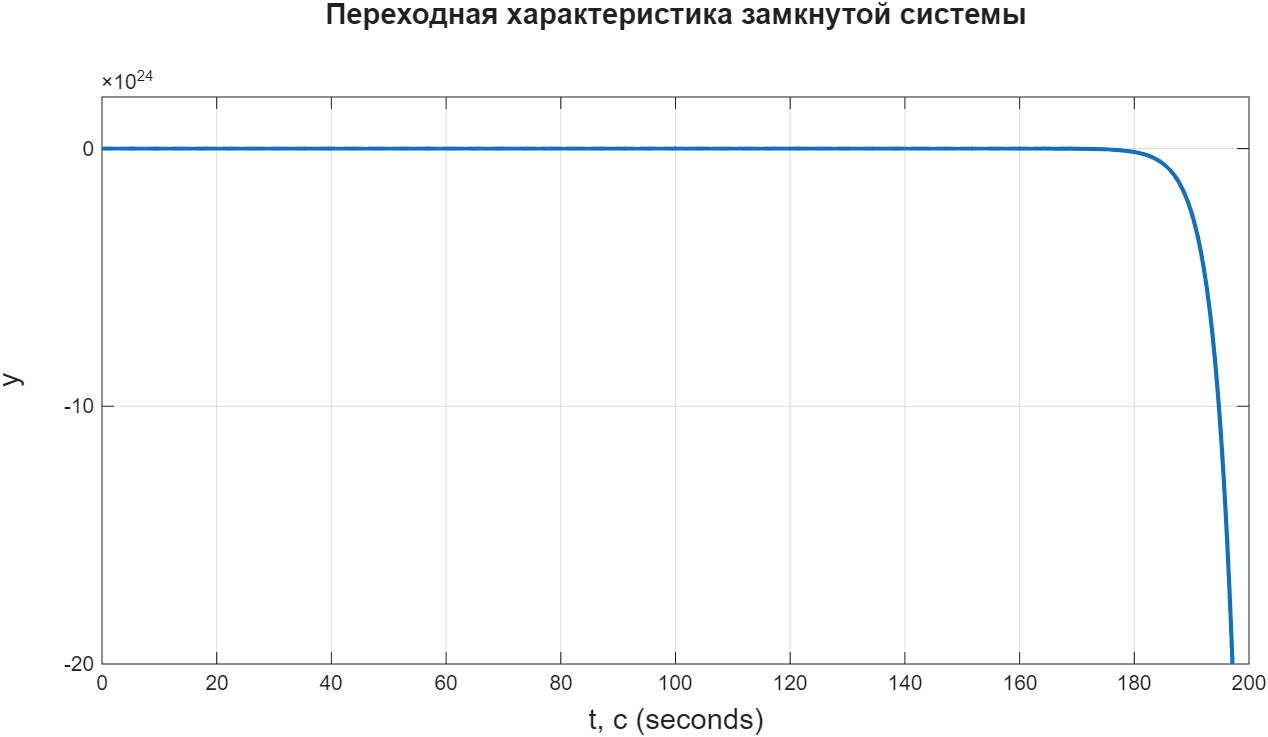
\includegraphics[width=0.75\linewidth]{images/Figure_6_2_1_10.png}
    \caption{Переходная характеристика при $k=4$ (1 передаточная функция)}
    \label{fig:placeholder}
\end{figure}

Как мы можем видеть на графиках, параметр k влияет на масштаб годографа Найквиста и если k будет больше 2.5, то он сможет сделать оборот вокруг точки по часовой стрелке из-за чего получится неустойчивый полюс замкнутой системы так как $n=0, \ N=1 \Rightarrow m-n=1$ и система станет неустойчивой, также это подтверждает переходная характеристика.

Рассмотрим зависимость корней характеристического уравнения замкнутой системы от k:

$$
\lambda^2+\lambda(6+k)+5-2k=0
$$

$$
\lambda=\dfrac{-6-k\pm\sqrt{(6+k)^2-20+8k}}{2}
$$

$$
\lambda=\dfrac{-6-k\pm\sqrt{k^2+20k+16}}{2}
$$

Получается, что корень:
$$\lambda=\dfrac{-6-k-\sqrt{k^2+20k+16}}{2}<0$$ 
при любых $k>0$ будет меньше нуля, тогда неустойчивым корнем может быть только:
$$\lambda=\dfrac{-6-k+\sqrt{k^2+20k+16}}{2}$$ 
и он будет неустойчивым в случае:
$$6+k<\sqrt{k^2+20k+16}$$

$$k^2+12k+36<k^2+20k+16$$

$$
k>2.5
$$

Получается, что при $k \in (0, 2.5]$ будет 0 неустойчивых полюсов и замкнутая система будет устойчива, а при $k>2.5$ система будет иметь 1 неустойчивый полюс будет неустойчива и годограф сделает один оборот по часовой стрелке вокруг точки $(1, 0)$. Моделирование подтвердило аналитические расчеты.

\begin{figure}[H]
    \centering
    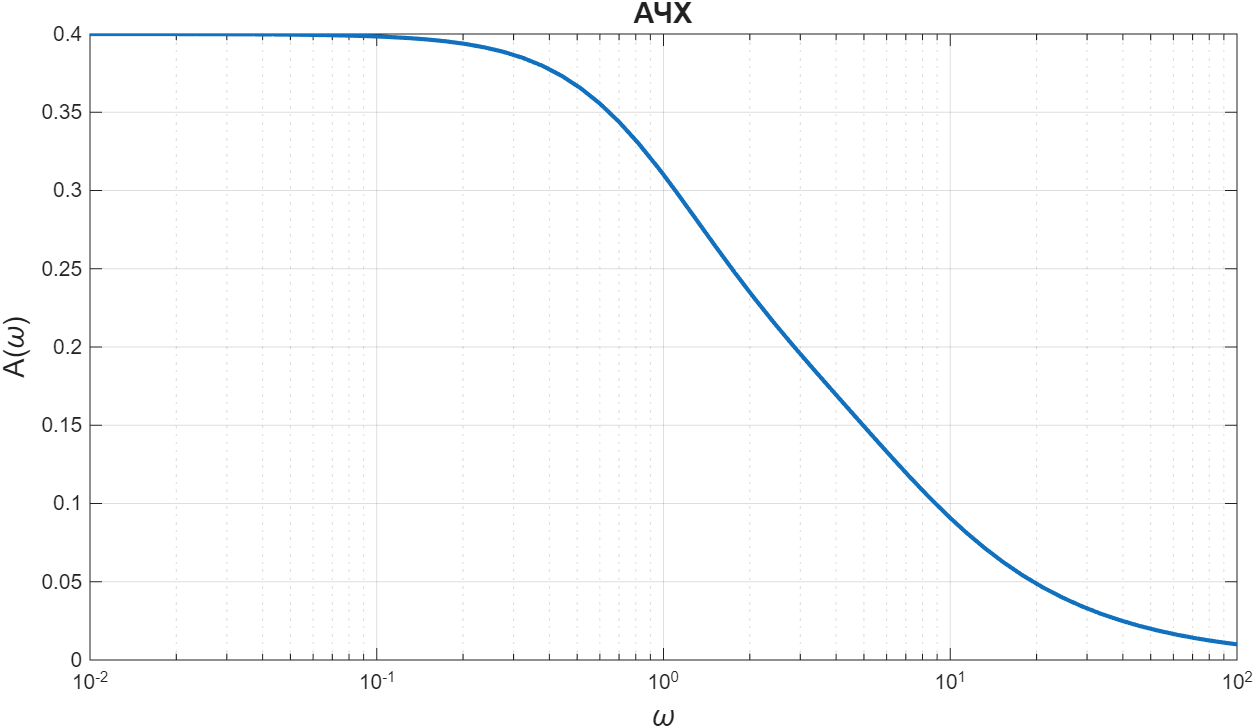
\includegraphics[width=0.75\linewidth]{images/Figure_6_2_1_11.png}
    \caption{АЧХ разомкнутой системы}
    \label{fig:placeholder}
\end{figure}

\begin{figure}[H]
    \centering
    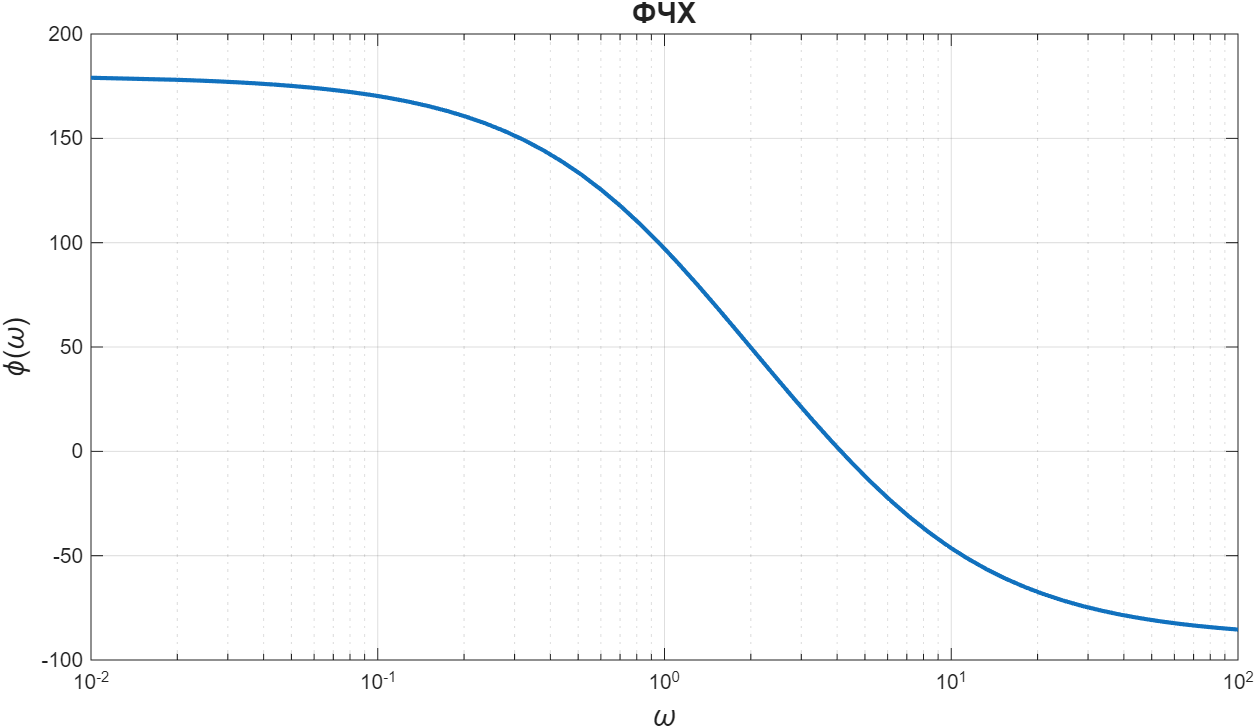
\includegraphics[width=0.75\linewidth]{images/Figure_6_2_1_12.png}
    \caption{ФЧХ разомкнутой системы}
    \label{fig:placeholder}
\end{figure}

Фаза равна $180^o$ при $\omega=0$, а $A(0)=0.4$, тогда $A_{\text{з}}=\dfrac{1}{0.4}=2.5$





\subsection{Вторая передаточная функция}

Домножим нашу передаточную функцию на коэффициент усисления $k$:

$$
W_2(s)=\dfrac{k(-9s^3+16s^2-6s)}{10s^3+12s^2+5s+1}
$$

Найдём корни характеристического уравнения разомкнутой системы $10s^3+12s^2+5s+1$:

\begin{figure}[H]
    \centering
    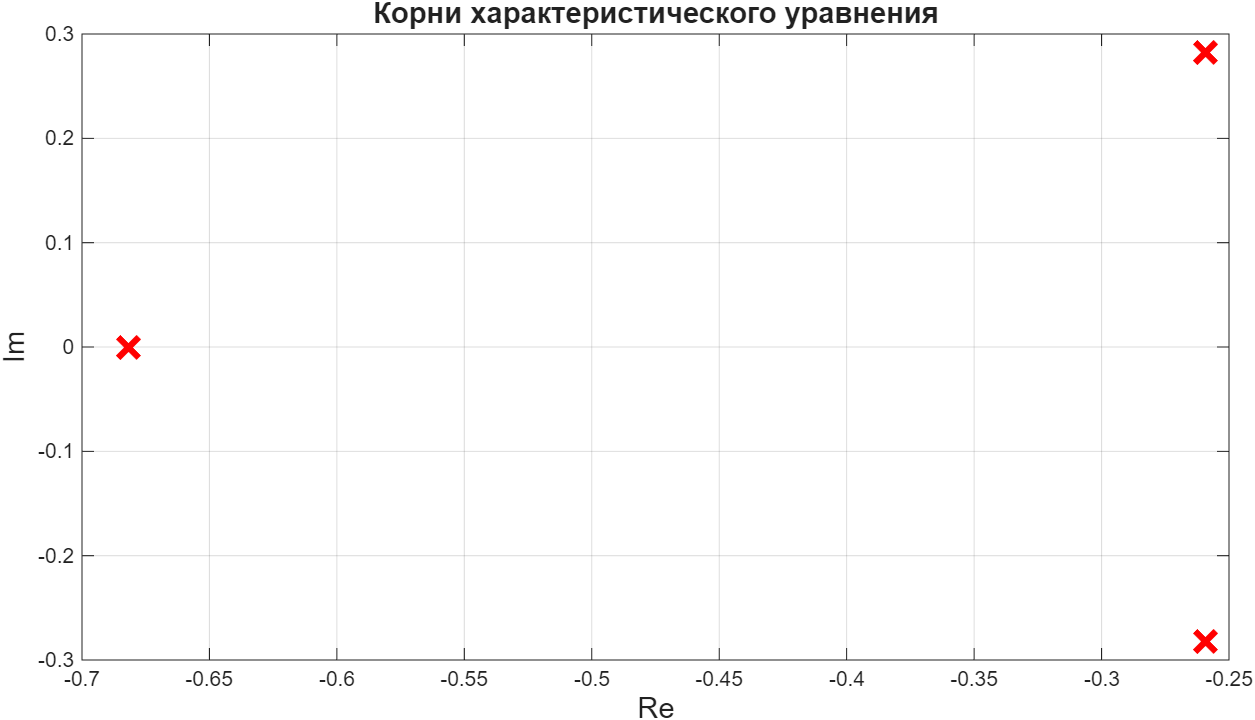
\includegraphics[width=0.75\linewidth]{images/Figure_6_2_2_1.png}
    \caption{Корни харатеристического уравнения разомкнутой системы}
    \label{fig:placeholder}
\end{figure}

Вещественная часть всех корней характеристического уравнения отрицательна $n=0$, следовательно для того чтобы замкнутая система стала неустойчивой годографу надо сделать хотябы один оборот по часовой стрелке вокруг точки (-1, 0)

Найдем передаточную функцию замкнутой системы:

$$
W_{\text{з}1}=\dfrac{\dfrac{k(-9s^3+16s^2-6s)}{10s^3+12s^2+5s+1}}{1+\dfrac{k(-9s^3+16s^2-6s)}{10s^3+12s^2+5s+1}}=\dfrac{k(-9s^3+16s^2-6s)}{s^3(10-9k)+s^2(12+16k)+s(5-6k)+1}
$$

\begin{figure}[H]
    \centering
    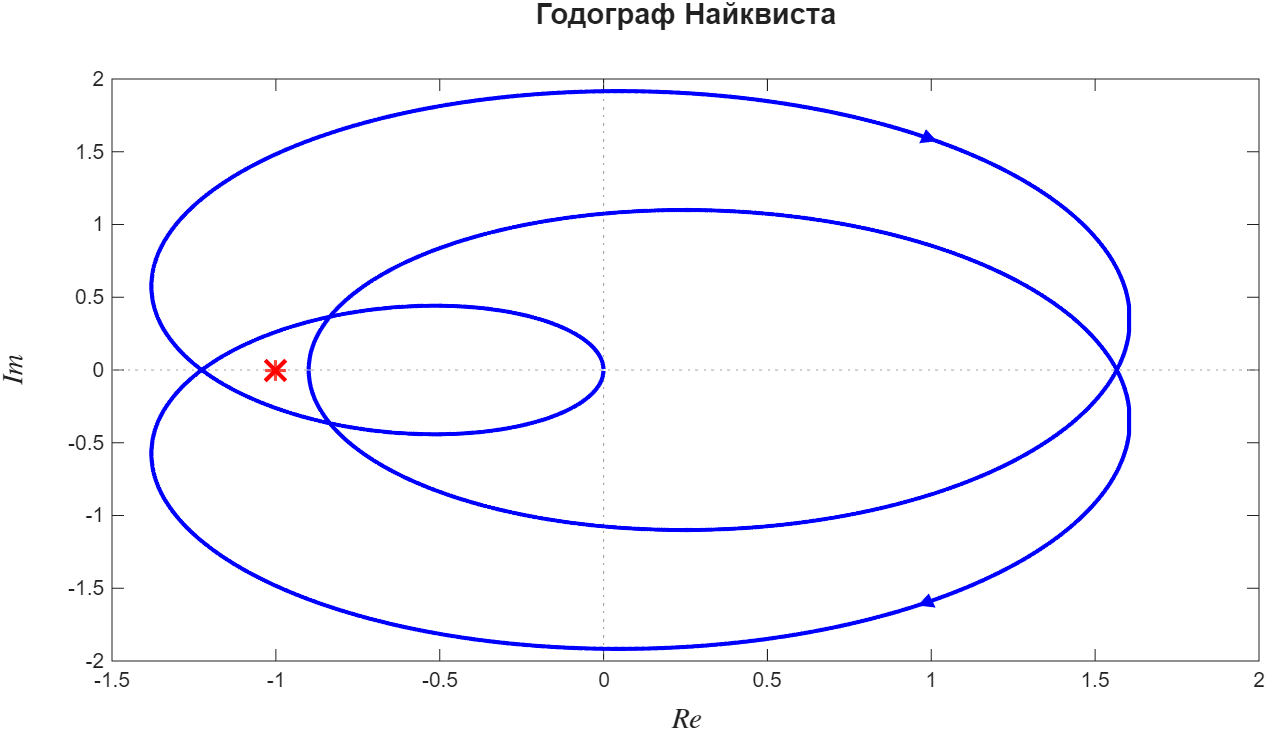
\includegraphics[width=0.75\linewidth]{images/Figure_6_2_2_2.png}
    \caption{Годограф Найквиста при $k=1$ (2 передаточная функция)}
    \label{fig:placeholder}
\end{figure}

По критерию Гурвинца система будет ассимптотически устойчива при:

$$
\begin{cases}
    \dfrac{12+16k}{10-9k}>0\\
    \\
    \dfrac{5-6k}{10-9k}>0\\
    \\
    10-9k>0\\
    \\
    \dfrac{(12+16k)}{10-9k}\dfrac{(5-6k)}{10-9k}>\dfrac{1}{10-9k}
\end{cases}
$$

$$
\begin{cases}
    k\in\left(-\dfrac{12}{16},\ \dfrac{10}{9}\right)\\
    k\in\left(-\infty, \ \dfrac{5}{6}\right)\\
    k\in\left(-\infty, \ \dfrac{10}{9}\right)\\
    k\in\left(\dfrac{-17+\sqrt{19489}}{-192}, \ \dfrac{-17-\sqrt{19489}}{-192}\right)
\end{cases}
$$

Так как по условию $k>0$ получаем промежуток при котором система будет ассимптотически устойчива: 

$$k\in (0,\ \dfrac{-17-\sqrt{19489}}{-192})$$

или:

$$
k\in (0,\ 0.8156)
$$


Выберем разные $k$:

$$
k=\{0.3,\ 0.7,\ 2,\ 3\}
$$

\begin{figure}[H]
    \centering
    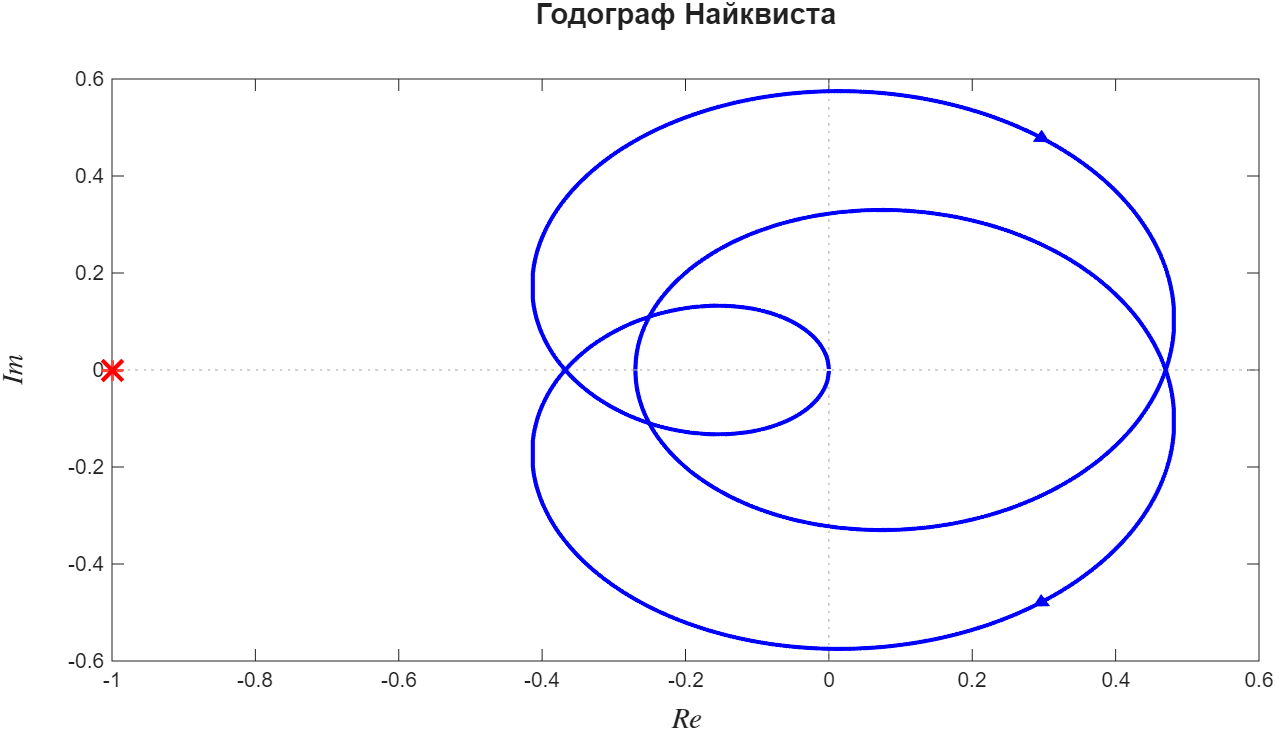
\includegraphics[width=0.75\linewidth]{images/Figure_6_2_2_3.png}
    \caption{Годограф Найквиста при $k=0.3$ (2 передаточная функция)}
    \label{fig:placeholder}
\end{figure}

\begin{figure}[H]
    \centering
    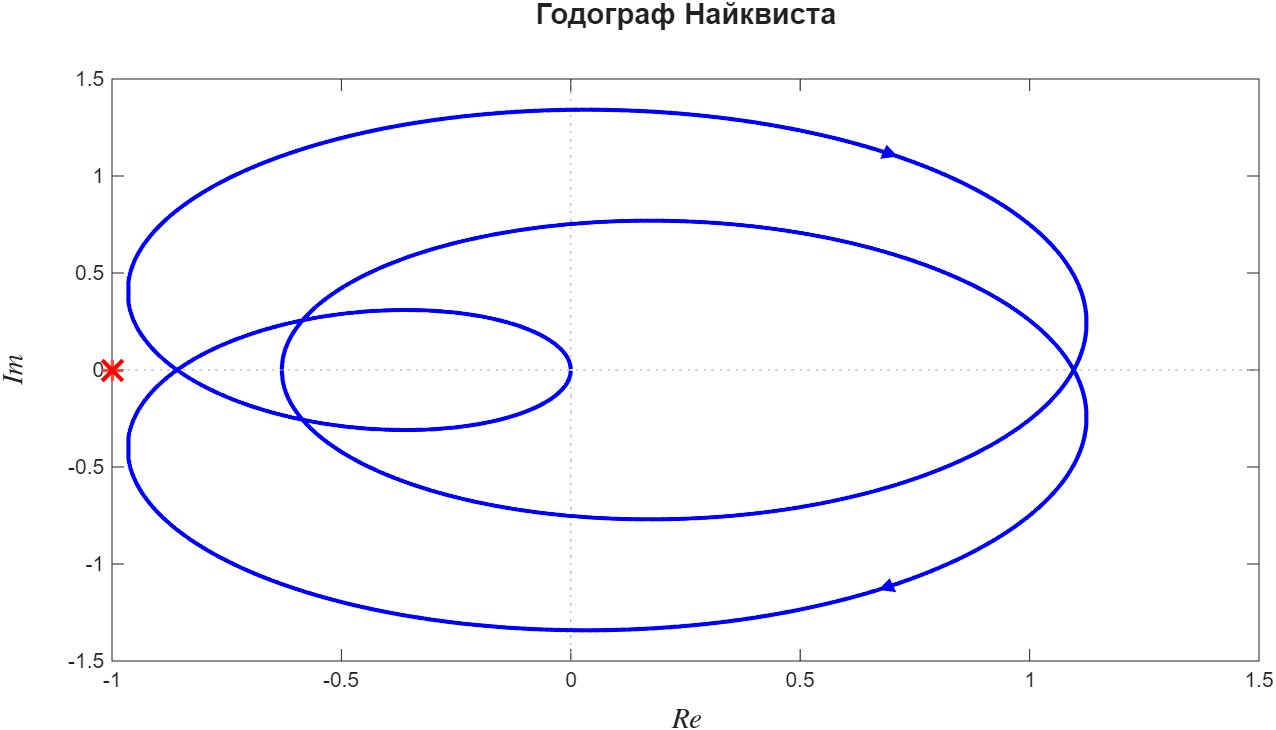
\includegraphics[width=0.75\linewidth]{images/Figure_6_2_2_4.png}
    \caption{Годограф Найквиста при $k=0.7$ (2 передаточная функция)}
    \label{fig:placeholder}
\end{figure}

\begin{figure}[H]
    \centering
    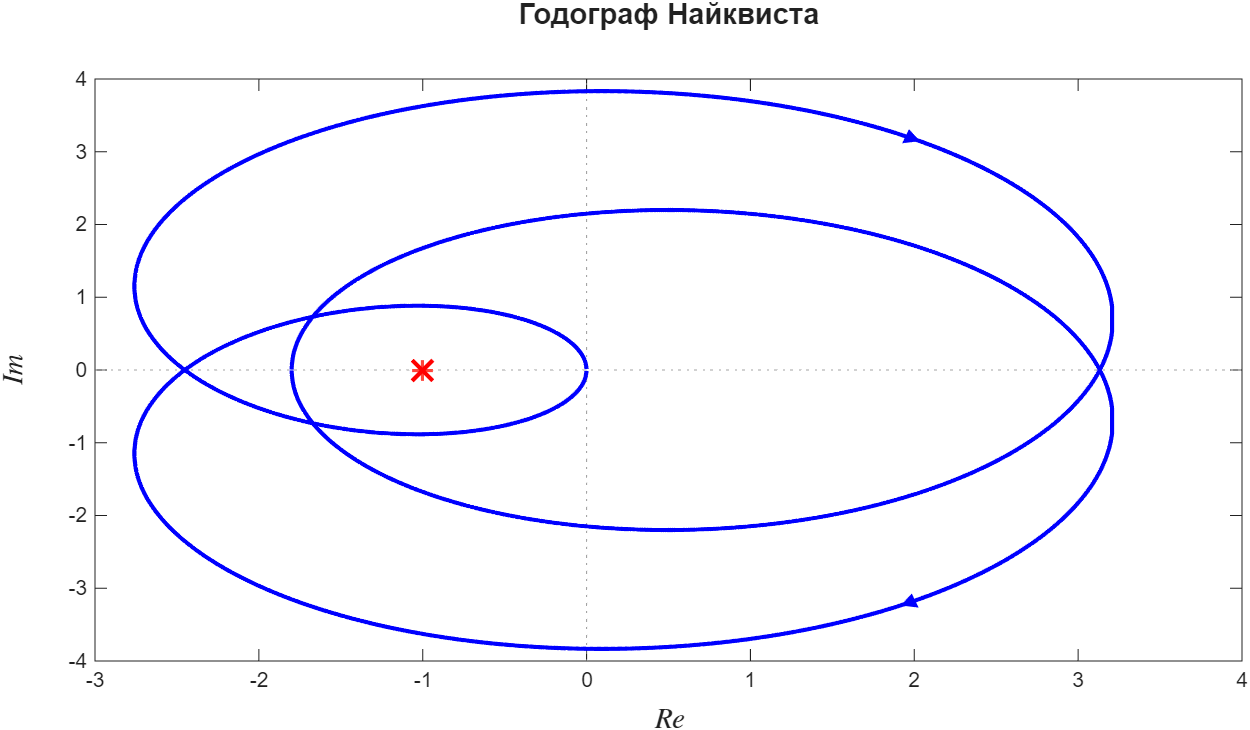
\includegraphics[width=0.75\linewidth]{images/Figure_6_2_2_5.png}
    \caption{Годограф Найквиста при $k=2$ (2 передаточная функция)}
    \label{fig:placeholder}
\end{figure}

\begin{figure}[H]
    \centering
    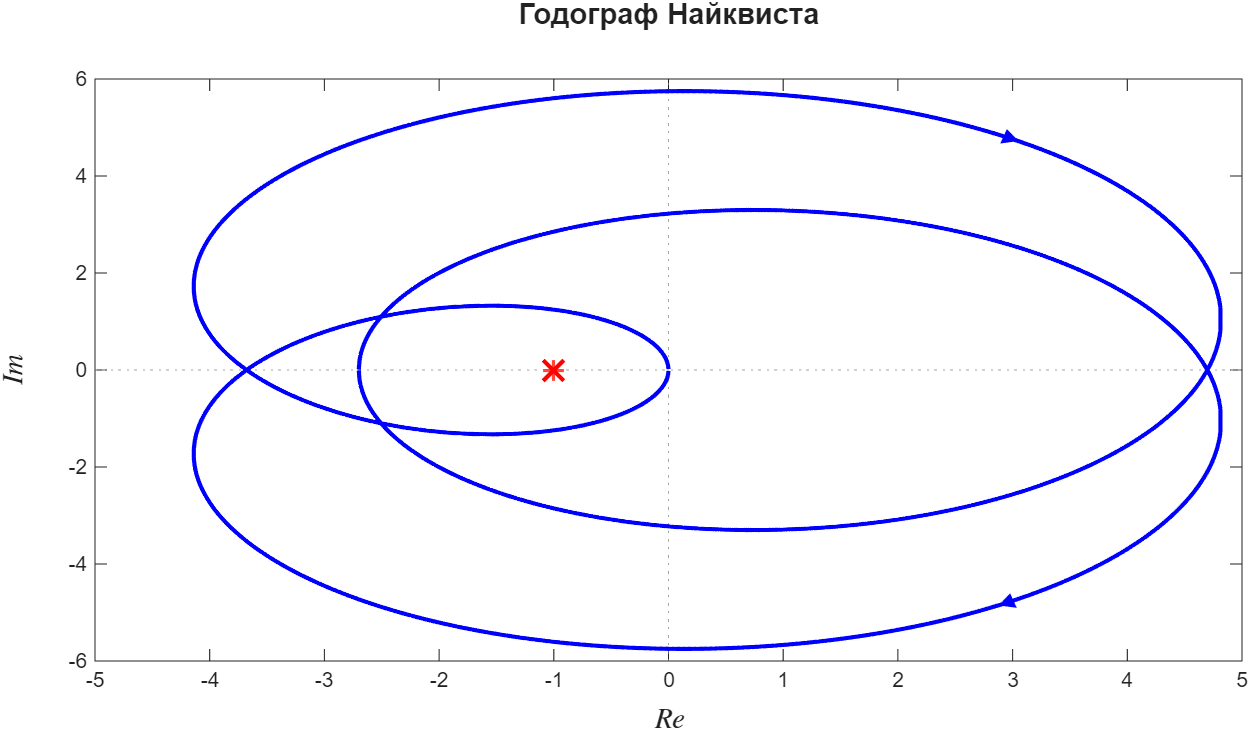
\includegraphics[width=0.75\linewidth]{images/Figure_6_2_2_6.png}
    \caption{Годограф Найквиста при $k=3$ (2 передаточная функция)}
    \label{fig:placeholder}
\end{figure}

\begin{figure}[H]
    \centering
    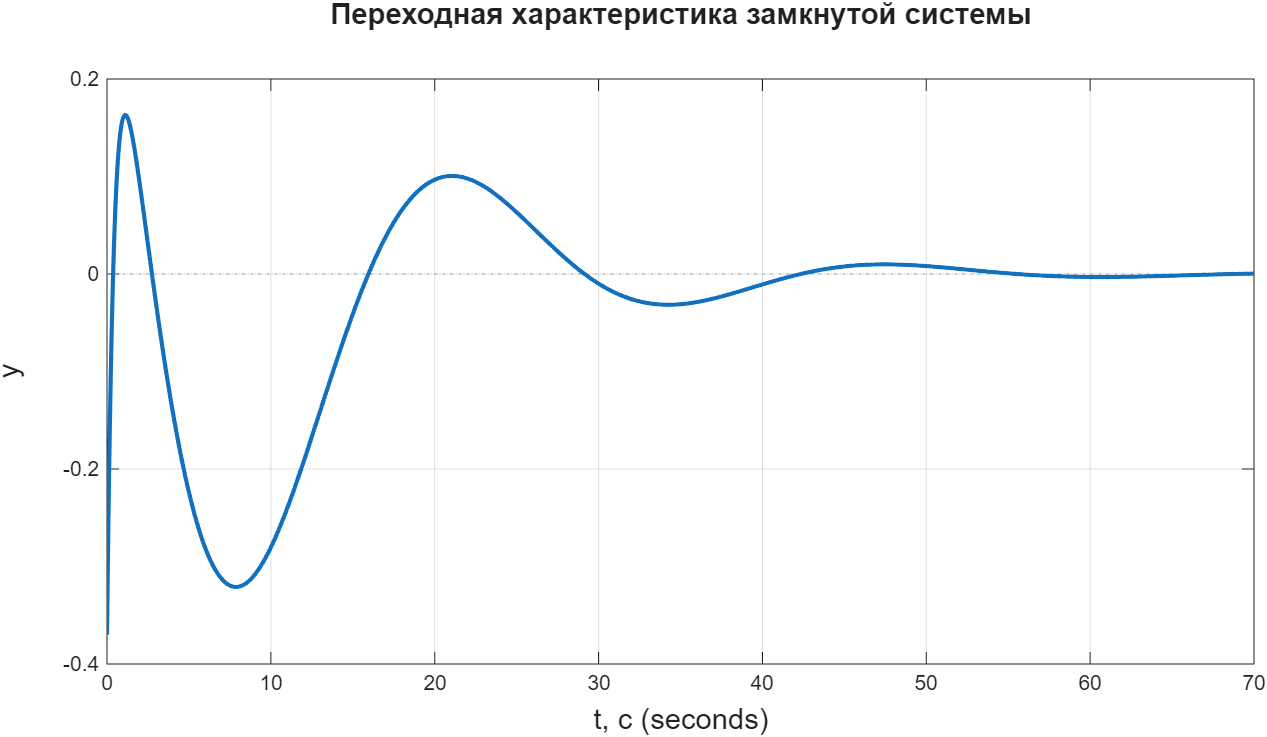
\includegraphics[width=0.75\linewidth]{images/Figure_6_2_2_7.png}
    \caption{Переходная характеристика при $k=0.3$ (2 передаточная функция)}
    \label{fig:placeholder}
\end{figure}

\begin{figure}[H]
    \centering
    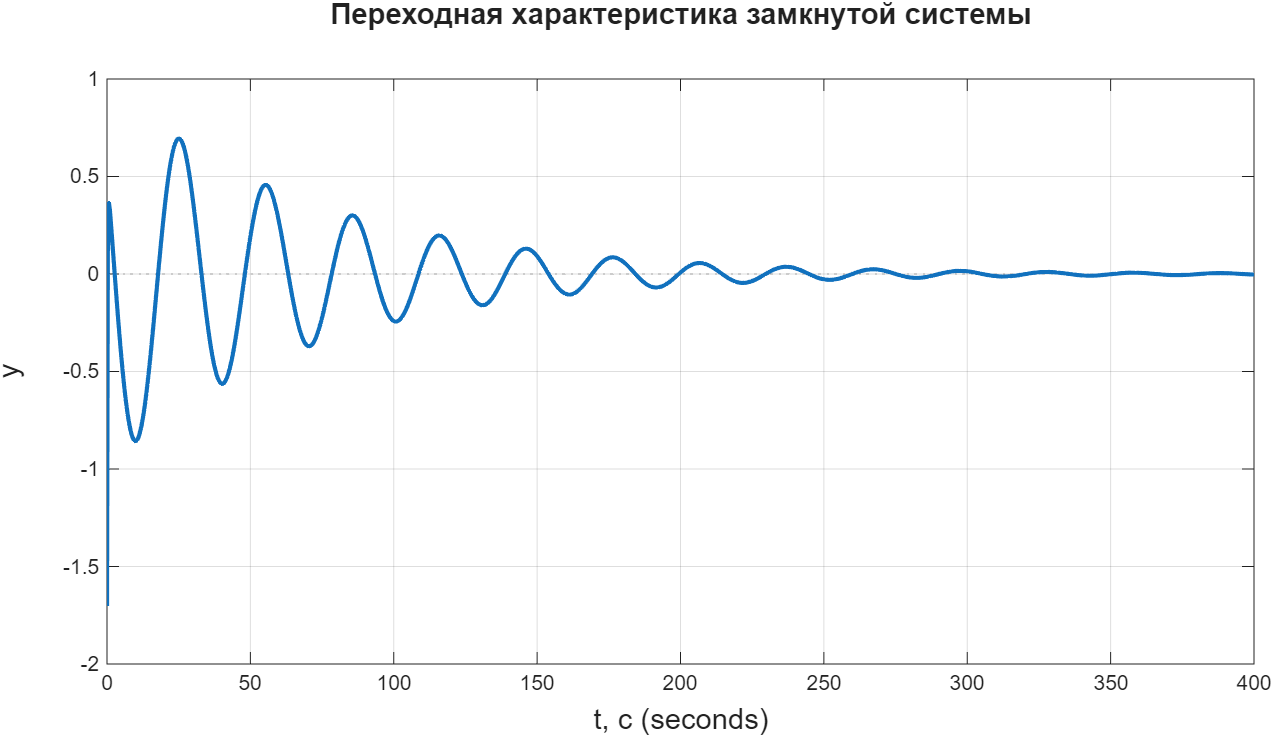
\includegraphics[width=0.75\linewidth]{images/Figure_6_2_2_8.png}
    \caption{Переходная характеристика при $k=0.7$ (2 передаточная функция)}
    \label{fig:placeholder}
\end{figure}

\begin{figure}[H]
    \centering
    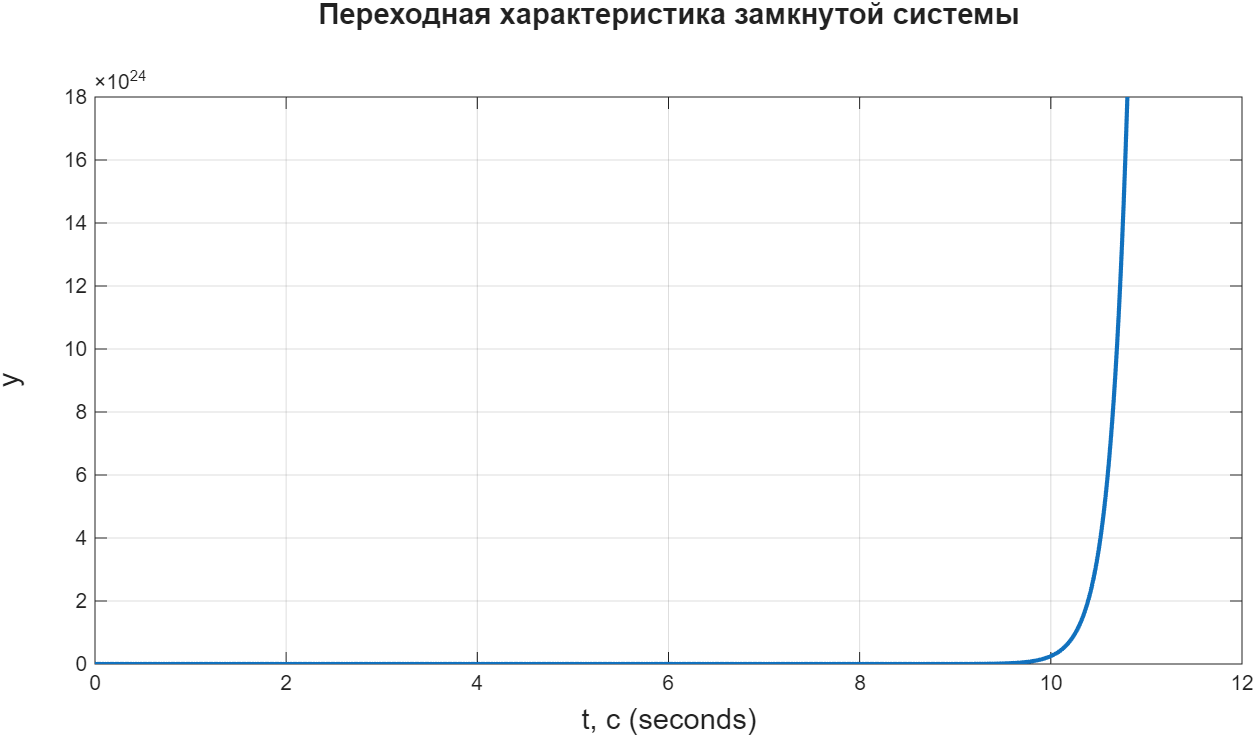
\includegraphics[width=0.75\linewidth]{images/Figure_6_2_2_9.png}
    \caption{Переходная характеристика при $k=2$ (2 передаточная функция)}
    \label{fig:placeholder}
\end{figure}

\begin{figure}[H]
    \centering
    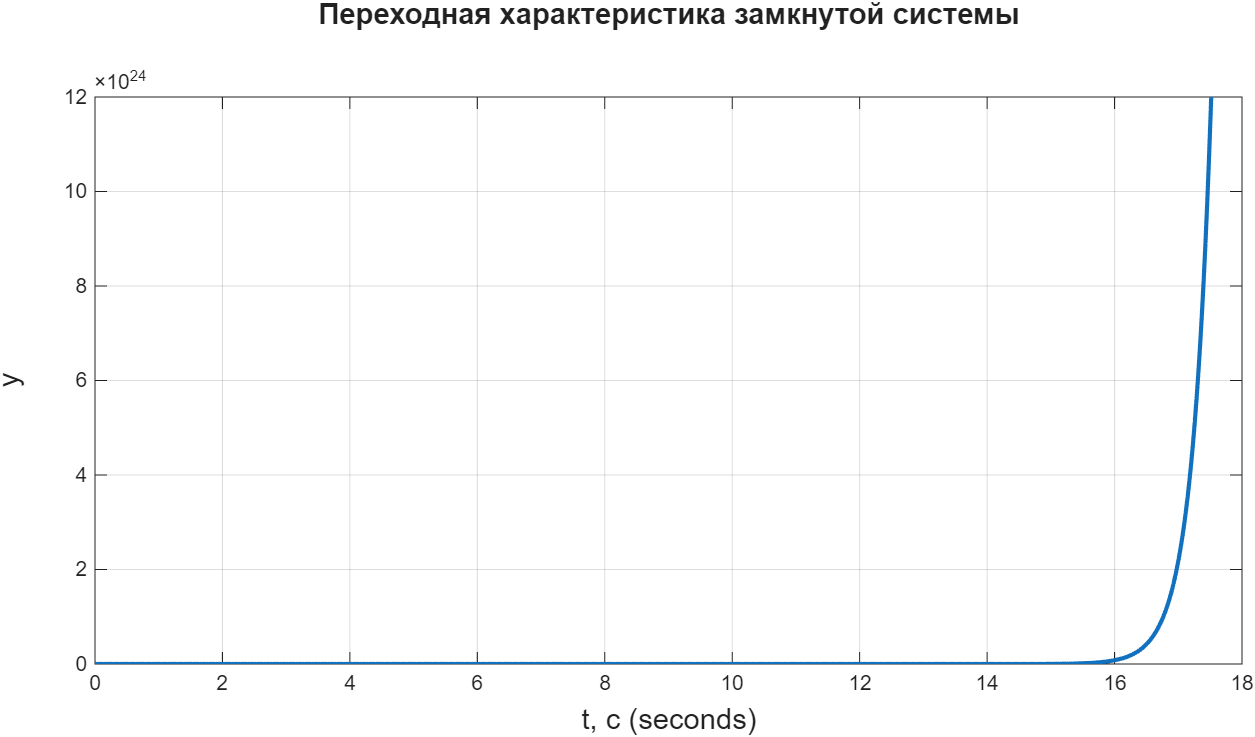
\includegraphics[width=0.75\linewidth]{images/Figure_6_2_2_10.png}
    \caption{Переходная характеристика при $k=3$ (2 передаточная функция)}
    \label{fig:placeholder}
\end{figure}

Как мы можем видеть на графиках, параметр k влияет на масштаб годографа Найквиста и если k будет больше 2.5, то он сможет сделать два или три оборота вокруг точки по часовой стрелке из-за чего получатся неустойчивые полюса замкнутой системы и система станет неустойчивой, также это подтверждает переходная характеристика.

Рассмотрим зависимость корней характеристического уравнения замкнутой системы от k, воспользовавшись тем же критерием Гурвинца:

$$
\begin{cases}
    k\in\left(-\dfrac{12}{16},\ \dfrac{10}{9}\right)\\
    k\in\left(-\infty, \ \dfrac{5}{6}\right)\\
    k\in\left(-\infty, \ \dfrac{10}{9}\right)\\
    k\in\left(\dfrac{-17+\sqrt{19489}}{-192}, \ \dfrac{-17-\sqrt{19489}}{-192}\right)
\end{cases}
$$

при $k>0$:

$$
\begin{cases}
    k\in\left(0,\ \dfrac{10}{9}\right)\\
    k\in\left(0, \ \dfrac{5}{6}\right)\\
    k\in\left(0, \ \dfrac{10}{9}\right)\\
    k\in\left(0, \ \dfrac{-17-\sqrt{19489}}{-192}\right)
\end{cases}
$$

Рассмотрим промежутки:
$$\left(0, \ \dfrac{-17-\sqrt{19489}}{-192}\right)\ \left(\dfrac{-17-\sqrt{19489}}{-192},\ \dfrac{5}{6}\right)\ \left(\dfrac{5}{6}, \ \dfrac{10}{9}\right)\ \left(\dfrac{10}{9}, \ +\infty\right)$$

На первом промежутке система не имеет неустойчивых полюсов по критерию Гурвинца. 

Корни характеристического уравнения на втором промежутке:

\begin{figure}[H]
    \centering
    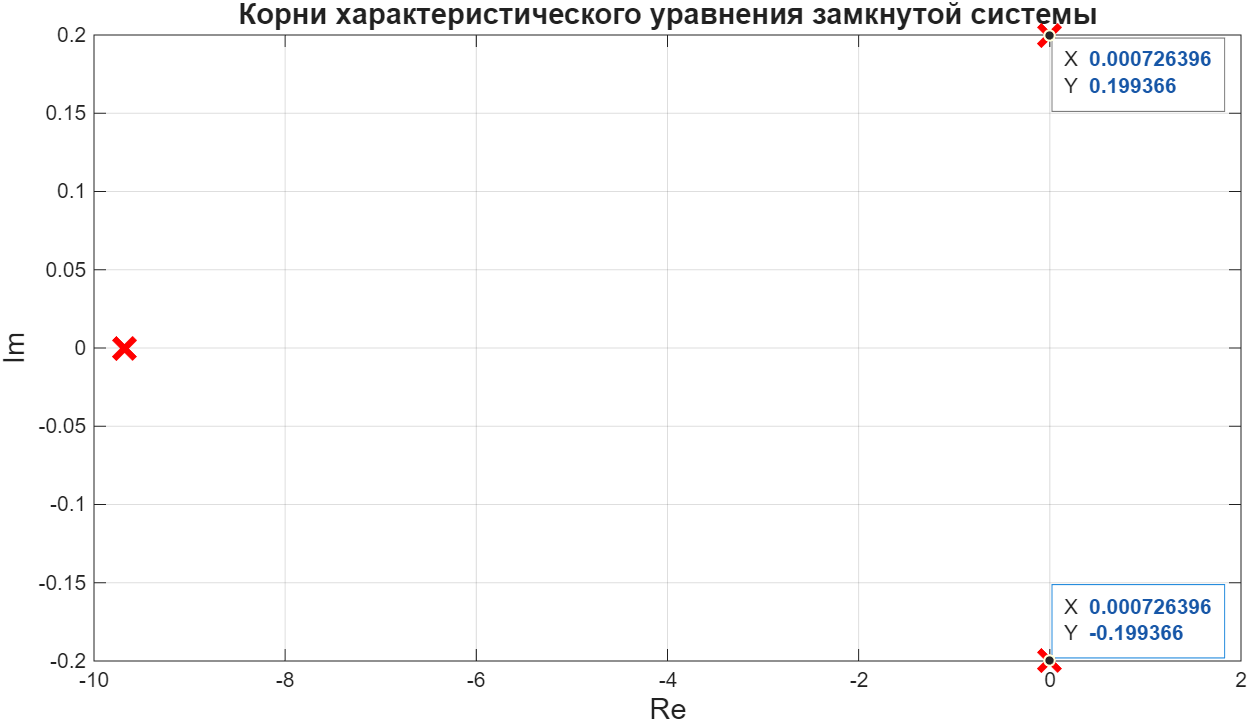
\includegraphics[width=0.75\linewidth]{images/Figure_6_2_2_11.png}
    \caption{Корни характеристического уравнения замкнутой системы}
    \label{fig:placeholder}
\end{figure}

На данном промежутке мы получаем 2 неустойчивых полюса.

\vspace{0.3cm}

Корни характеристического уравнения на третьем промежутке:

\begin{figure}[H]
    \centering
    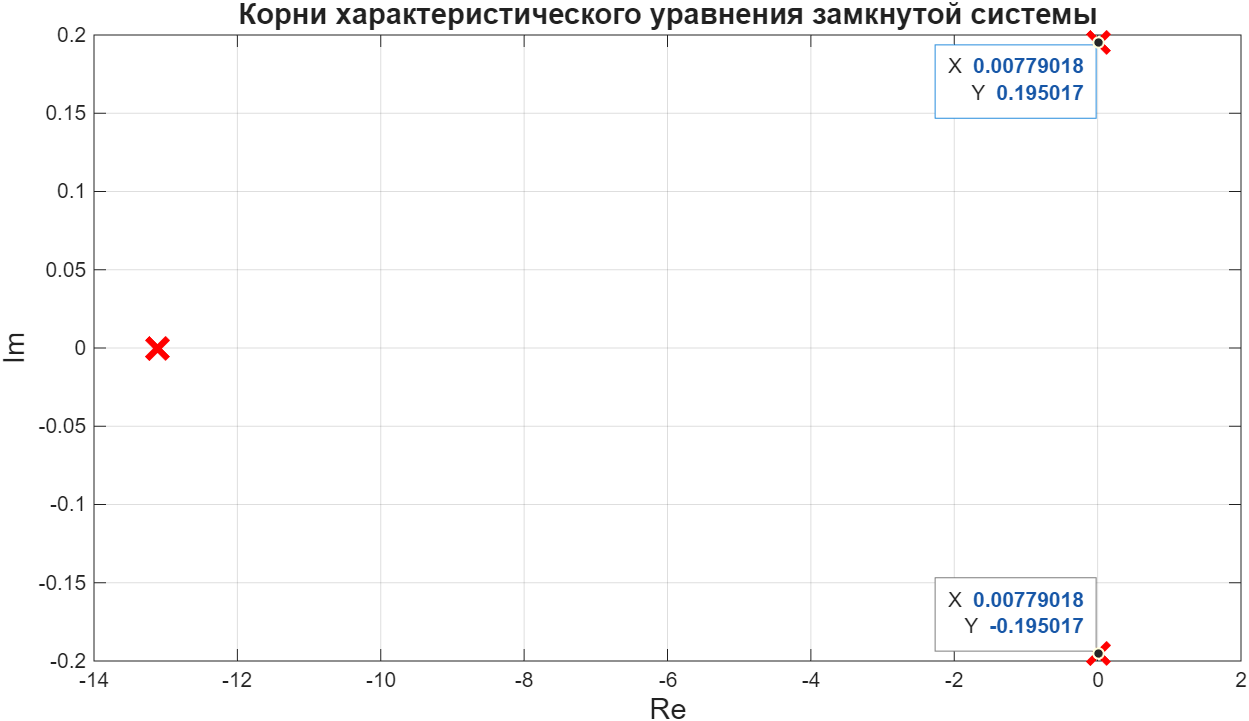
\includegraphics[width=0.75\linewidth]{images/Figure_6_2_2_12.png}
    \caption{Корни характеристического уравнения замкнутой системы}
    \label{fig:placeholder}
\end{figure}

На данном промежутке мы также получаем 2 неустойчивых полюса.

\vspace{0.3cm}

Корни характеристического уравнения на четвертом промежутке:

\begin{figure}[H]
    \centering
    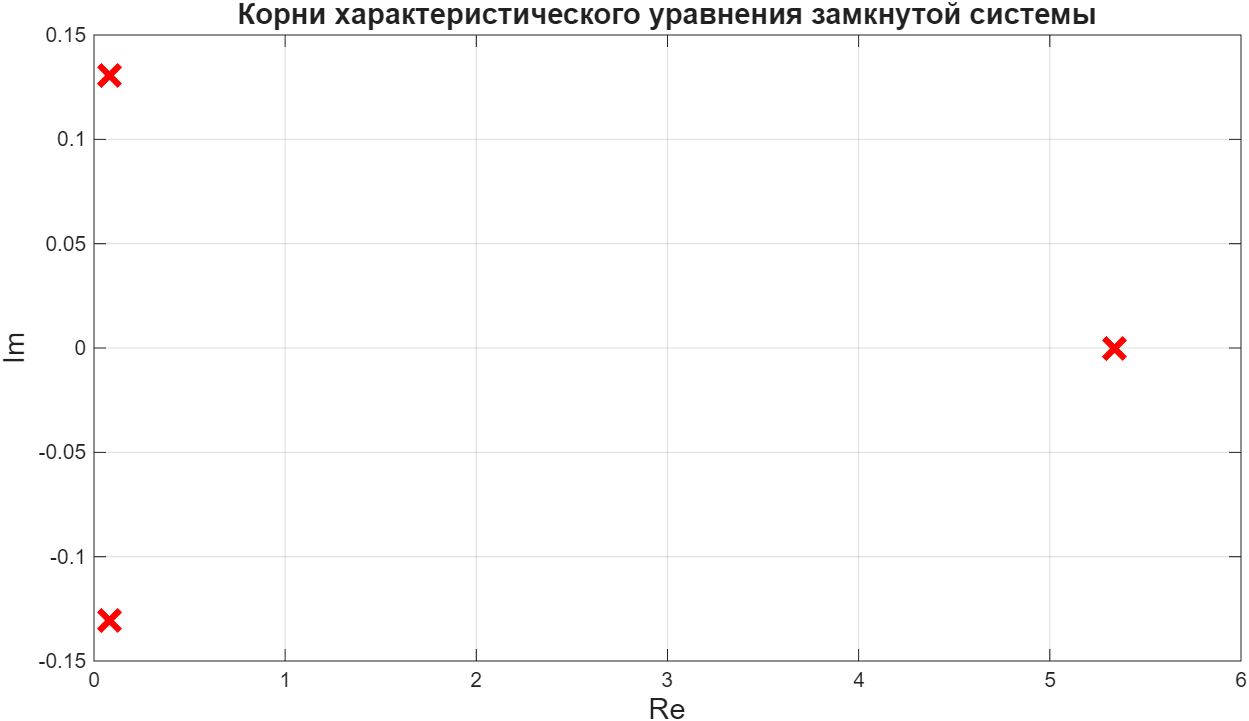
\includegraphics[width=0.75\linewidth]{images/Figure_6_2_2_13.png}
    \caption{Корни характеристического уравнения замкнутой системы}
    \label{fig:placeholder}
\end{figure}

На данном промежутке мы получаем 3 неустойчивых полюса.

Получается, что 0 неустойчивых полюсов мы получаем на промежутке:

$$
\left(0, \ \dfrac{-17-\sqrt{19489}}{-192}\right)
$$

2 неустойчивых полюса мы получаем на промежутке:

$$
\left(\dfrac{-17-\sqrt{19489}}{-192},\ \dfrac{10}{9}\right)
$$

3 неустойчивых полюса мы получаем на промежутке:

$$
\left(\dfrac{10}{9}, \ +\infty\right)
$$

Моделирование подтвердило аналитические расчеты.

Так как при $k=1$ система неустойчивая, то запаса устойчивости по амплитуде нет.



\newpage

\section{Задание 3. Запаздывание}

\subsection{Исходные данные:}
\begin{center}
\begin{tabular}{|c|c|}
\hline
     Параметр & Значение \\ \hline
     p&3\\ \hline
     q&2\\ \hline
     n&4\\ \hline
     m&4\\ \hline
     i&2\\ \hline
     j&6\\ \hline
\end{tabular}
\end{center}

\begin{center}
\begin{tabular}{|c|c|}
\hline
     $W_3(s)$ & $W_4(s)$ \\ \hline
     $\dfrac{9s+3}{s^2+3s+5}$&$\dfrac{10s^2-6s+11}{10s^3-s^2+38s+20}$\\ \hline
\end{tabular}
\end{center}

\subsection{Третья передаточная функция}

Добавим к передаточной функции звено чистого запаздывания:

$$
W(s)=e^{-\tau s}\dfrac{9s+3}{s^2+3s+5}
$$

Полюса разомкнутой системы:

\begin{figure}[H]
    \centering
    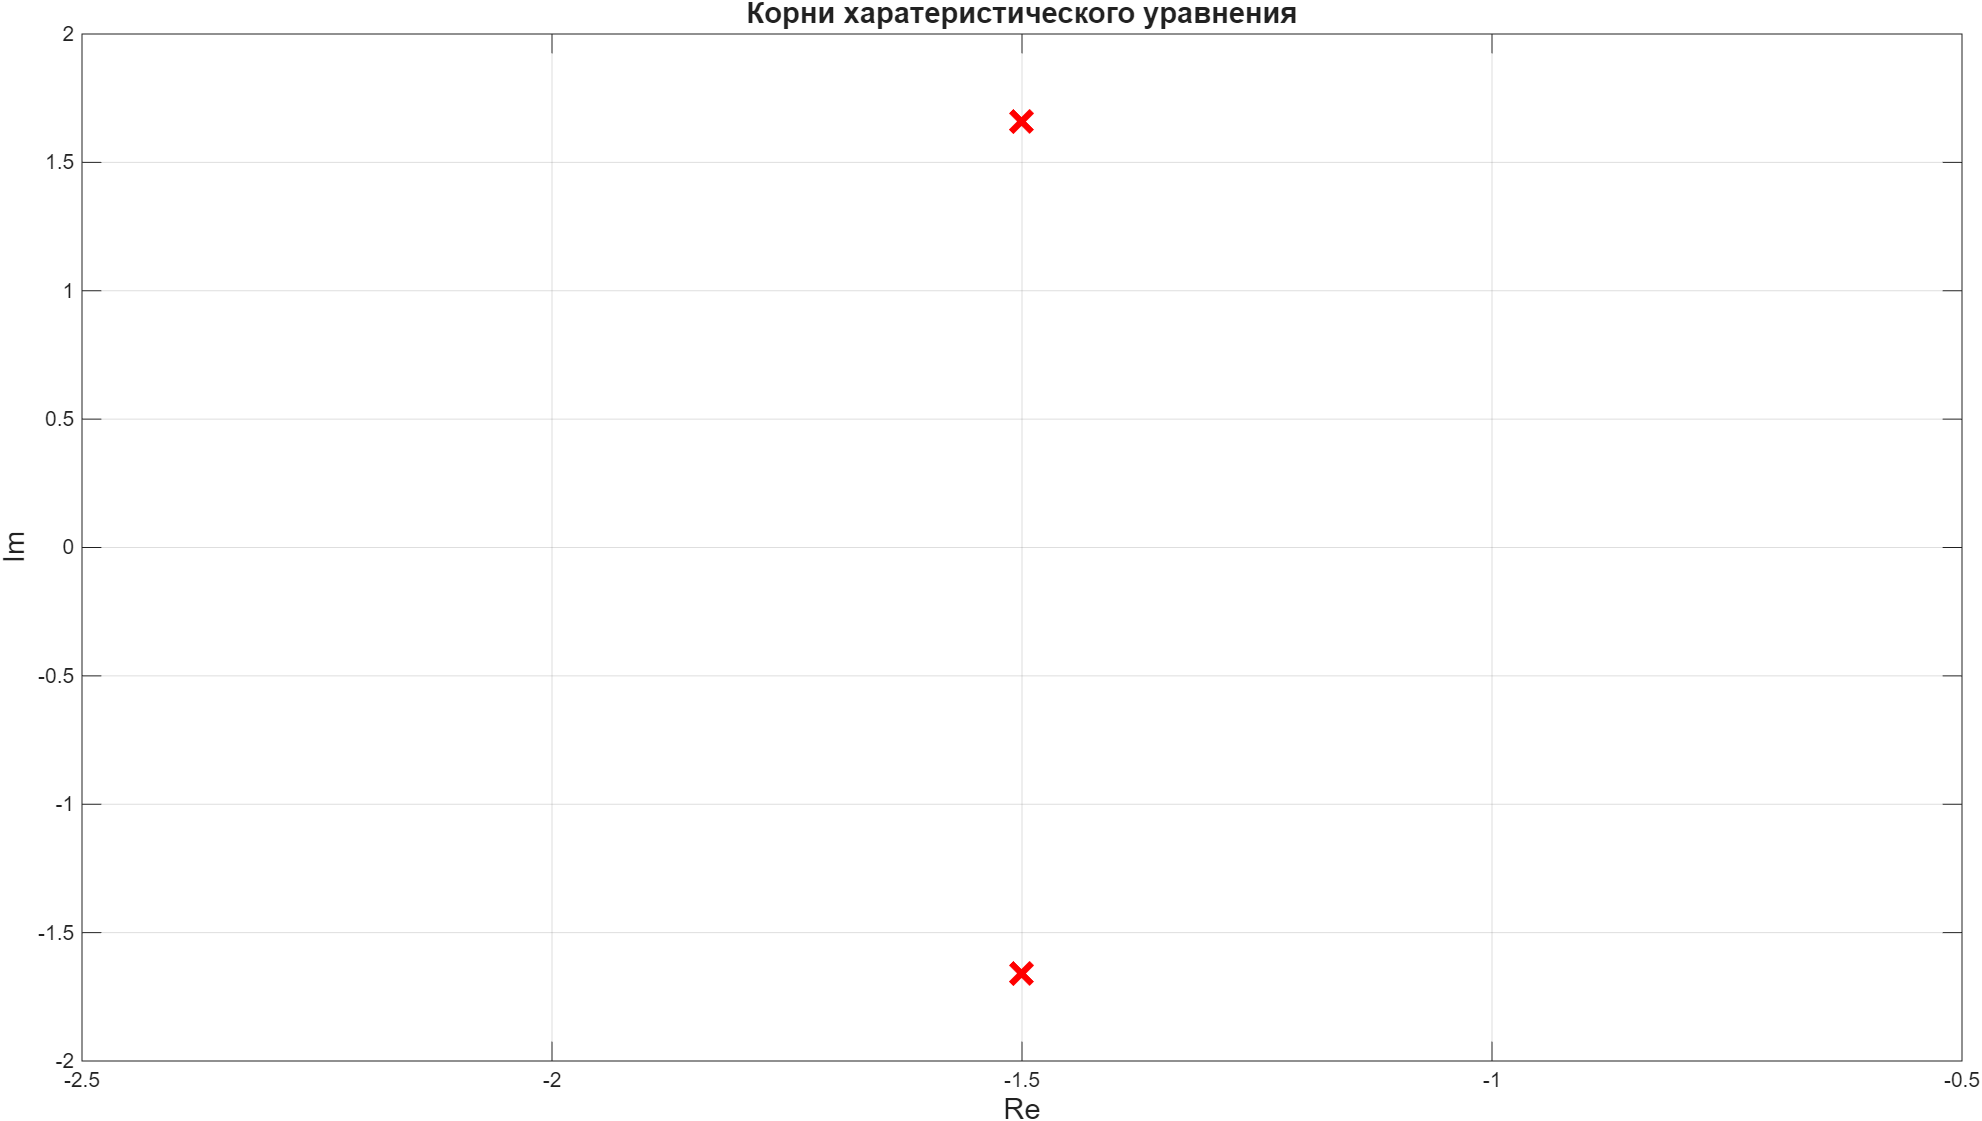
\includegraphics[width=0.75\linewidth]{images/Figure_6_3_1_1.png}
    \caption{Корни характеристического уравнения (3 передаточная функция)}
    \label{fig:placeholder}
\end{figure}

Разомкнутая система ассимптотически устойчива

\begin{figure}[H]
    \centering
    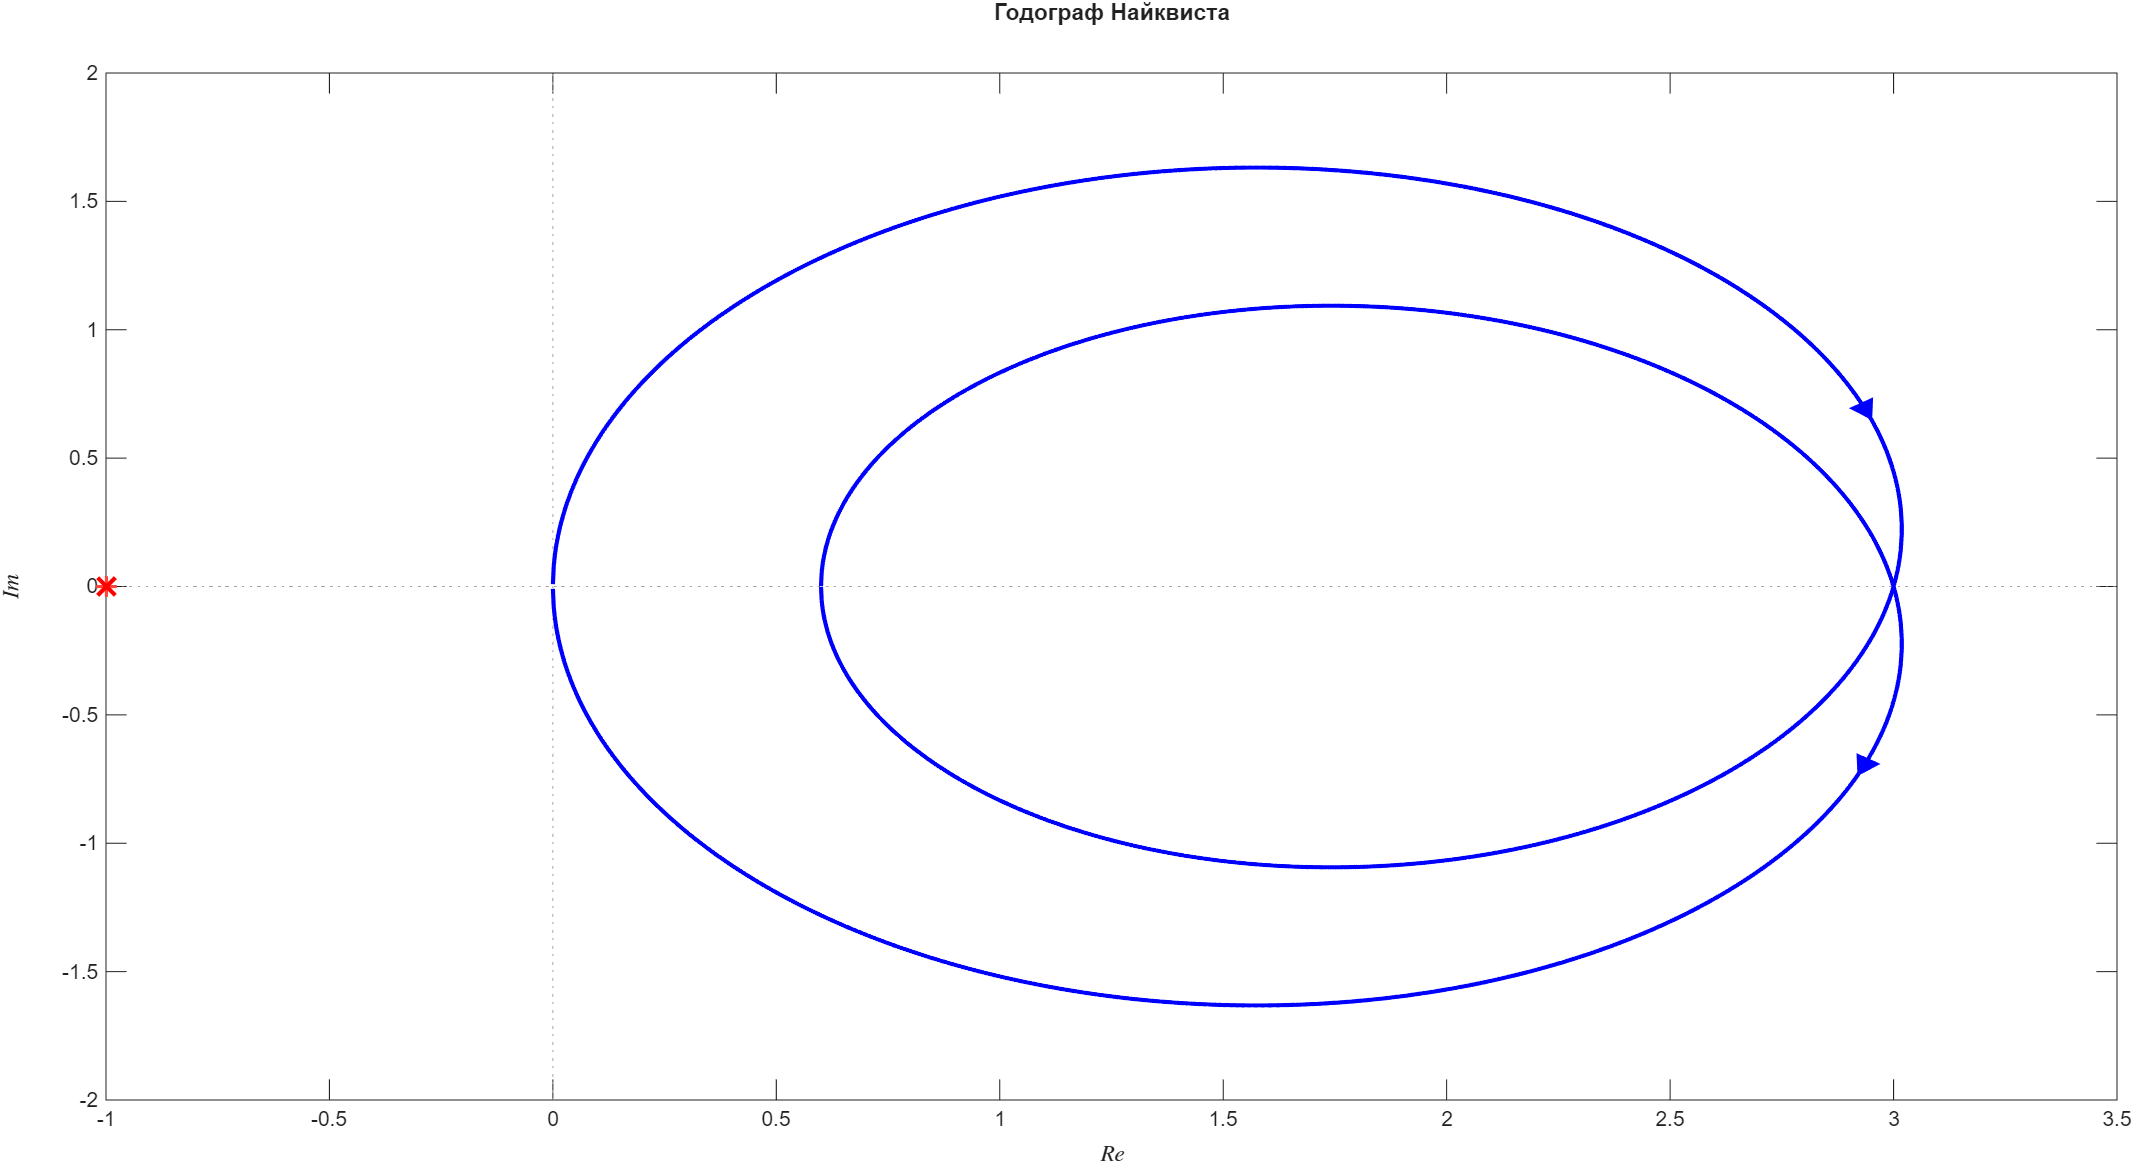
\includegraphics[width=0.75\linewidth]{images/Figure_6_3_1_2.png}
    \caption{Годограф Найквиста при $\tau = 0$ (3 передаточная функция)}
    \label{fig:placeholder}
\end{figure}

\begin{figure}[H]
    \centering
    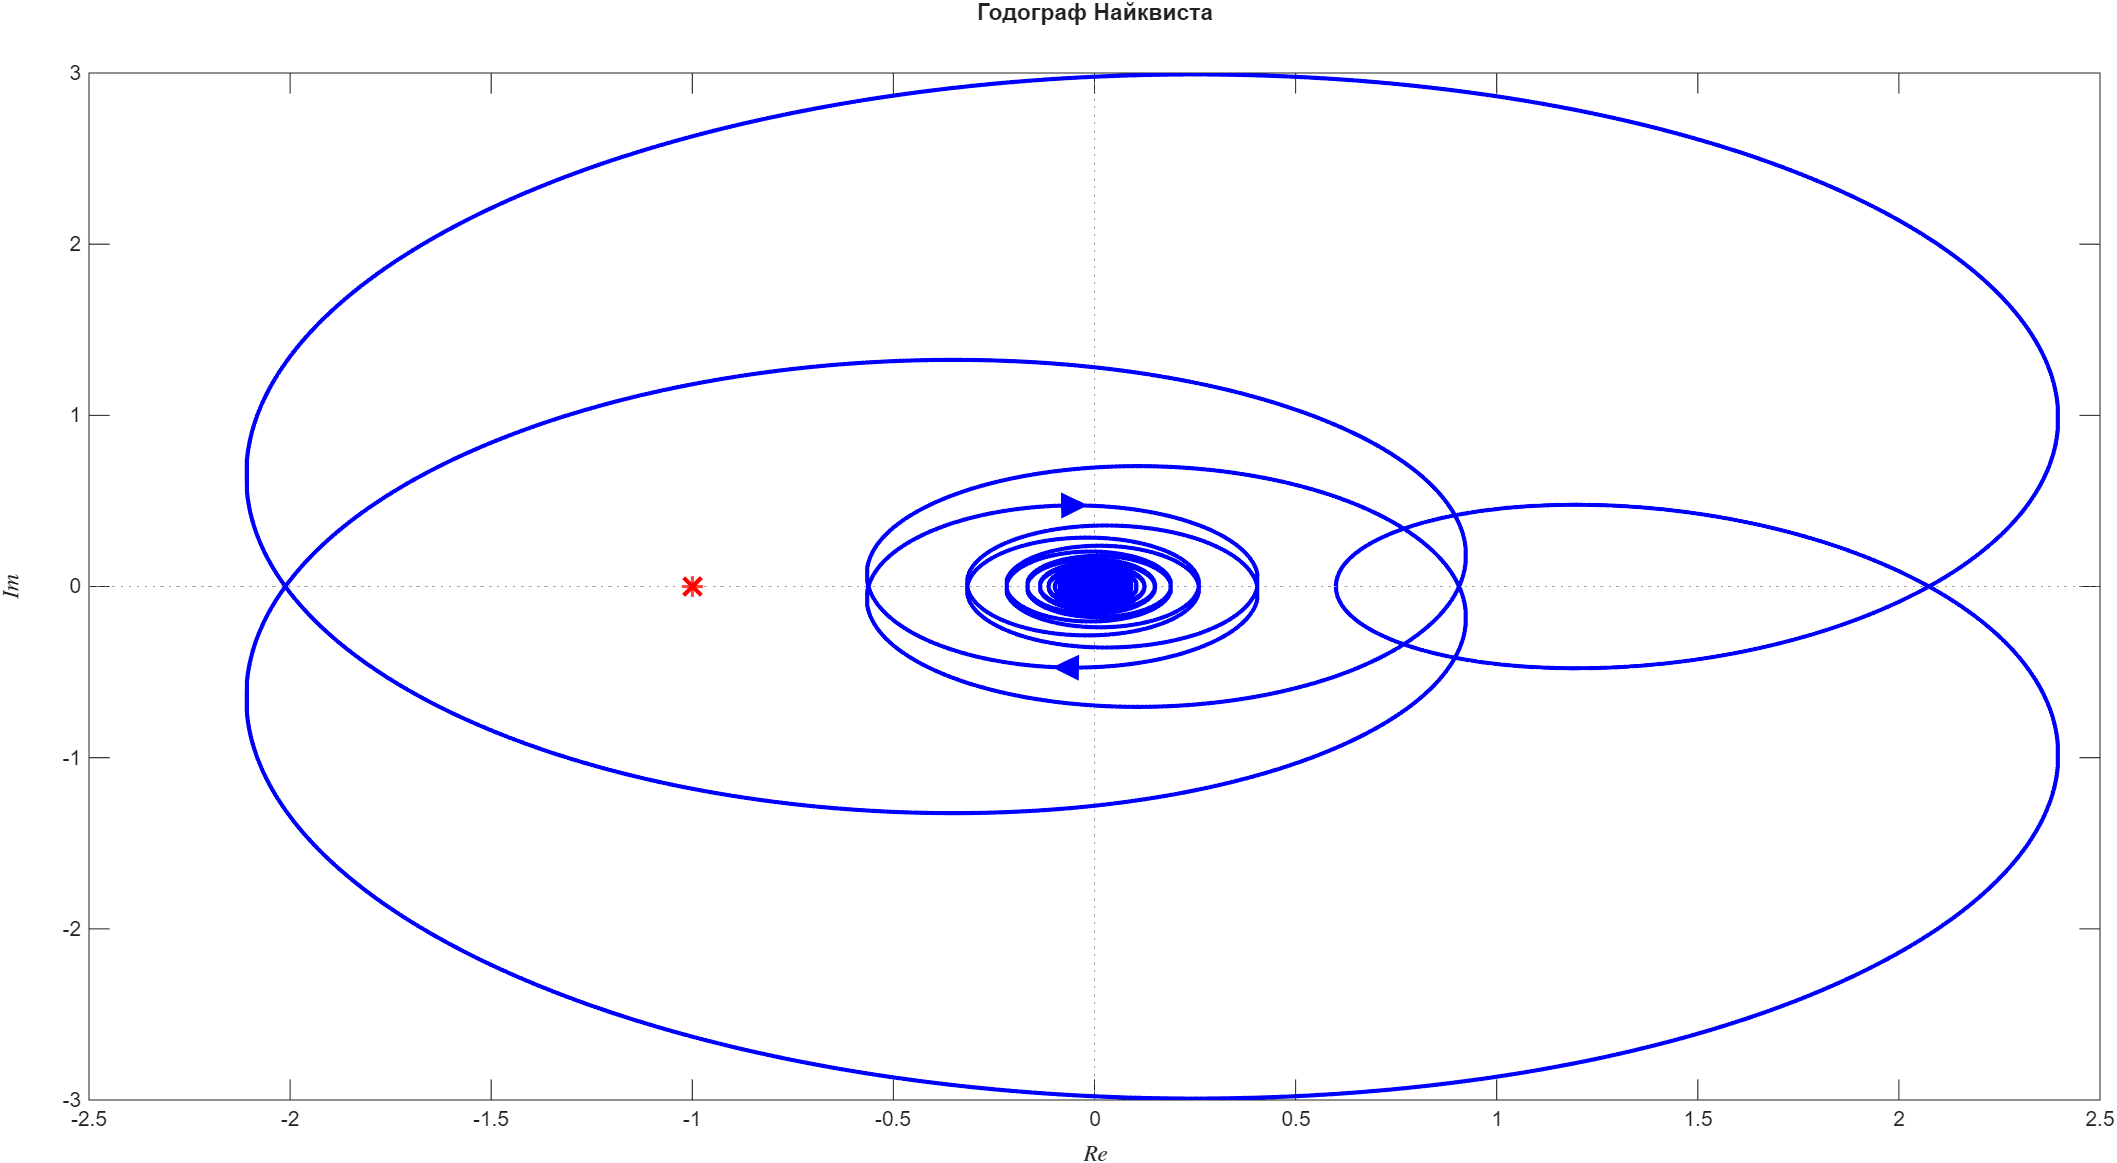
\includegraphics[width=0.75\linewidth]{images/Figure_6_3_1_3.png}
    \caption{Годограф Найквиста при $\tau = 0.5$ (3 передаточная функция)}
    \label{fig:placeholder}
\end{figure}

Частотная передаточная функция:

\[
W(j\omega) = \frac{3 + j9\omega}{(5 - \omega^2) + j3\omega}
\]

Найдём амплитуду:

\[
|W(j\omega)| = \dfrac{|3 + j9\omega|}{|(5 - \omega^2) + j3\omega|} = \frac{3\sqrt{1 + 9\omega^2}}{\sqrt{\omega^4 - \omega^2 + 25}}
\]

При $|W(j\omega_c)| = 1$:
\[
\frac{3\sqrt{1 + 9\omega_c^2}}{\sqrt{\omega_c^4 - \omega_c^2 + 25}} = 1
\]

Возводим в квадрат:
\[
9(1 + 9\omega_c^2) = \omega_c^4 - \omega_c^2 + 25
\]
\[
9 + 81\omega_c^2 = \omega_c^4 - \omega_c^2 + 25
\]

\[
\omega_c^4 - 82\omega_c^2 + 16 = 0
\]

Корни квадратного уравнения:
$$
\omega_1 \approx 0.443 \text{ рад/с}, \quad \omega_2 \approx 9.045 \text{ рад/с}
$$

Рассчитаем фазу:

\vspace{0.3cm}

Для $\omega_1 \approx 0.443$ рад/с:
$$
\varphi(\omega_1) = \arg(9j\omega_1 + 3) - \arg(5 - \omega_1^2 + 3j\omega_1)
$$
$$
\varphi(\omega_1) \approx 0.198 \text{ рад} \approx 11.3^{\circ}
$$

Для $\omega_2 \approx 9.045$ рад/с:
$$
\varphi(\omega_2) = \arg(9j\omega_2 + 3) - \arg(5 - \omega_2^2 + 3j\omega_2)
$$
$$
\varphi(\omega_2) \approx -1.268 \text{ рад} \approx -72.7^{\circ}
$$

Найдём значения критического запаздывания

\vspace{0.3cm}

Для $\omega_1$:
$$
\tau_{\text{кр1}} = \dfrac{\pi + \varphi(\omega_1)}{\omega_1} \approx \dfrac{3.142 + 0.198}{0.443} \approx 8.62 \text{ с}
$$

Для $\omega_2$:
$$
\tau_{\text{кр2}} = \dfrac{\pi + \varphi(\omega_2)}{\omega_2} \approx \dfrac{3.142 - 1.268}{9.045} \approx 0.207 \text{ с}
$$

Система устойчива при:
$$
0 \le \tau < 0.207
$$


Запас по фазе:
\[
\varphi_{\text{з}} = \pi + \varphi(\omega_{\text{с}}) \approx 107.3^\circ
\]

Возьмем $\tau =\{0.05,\ 0.1,\ 0.6,\ 0.8  \}$

\begin{figure}[H]
    \centering
    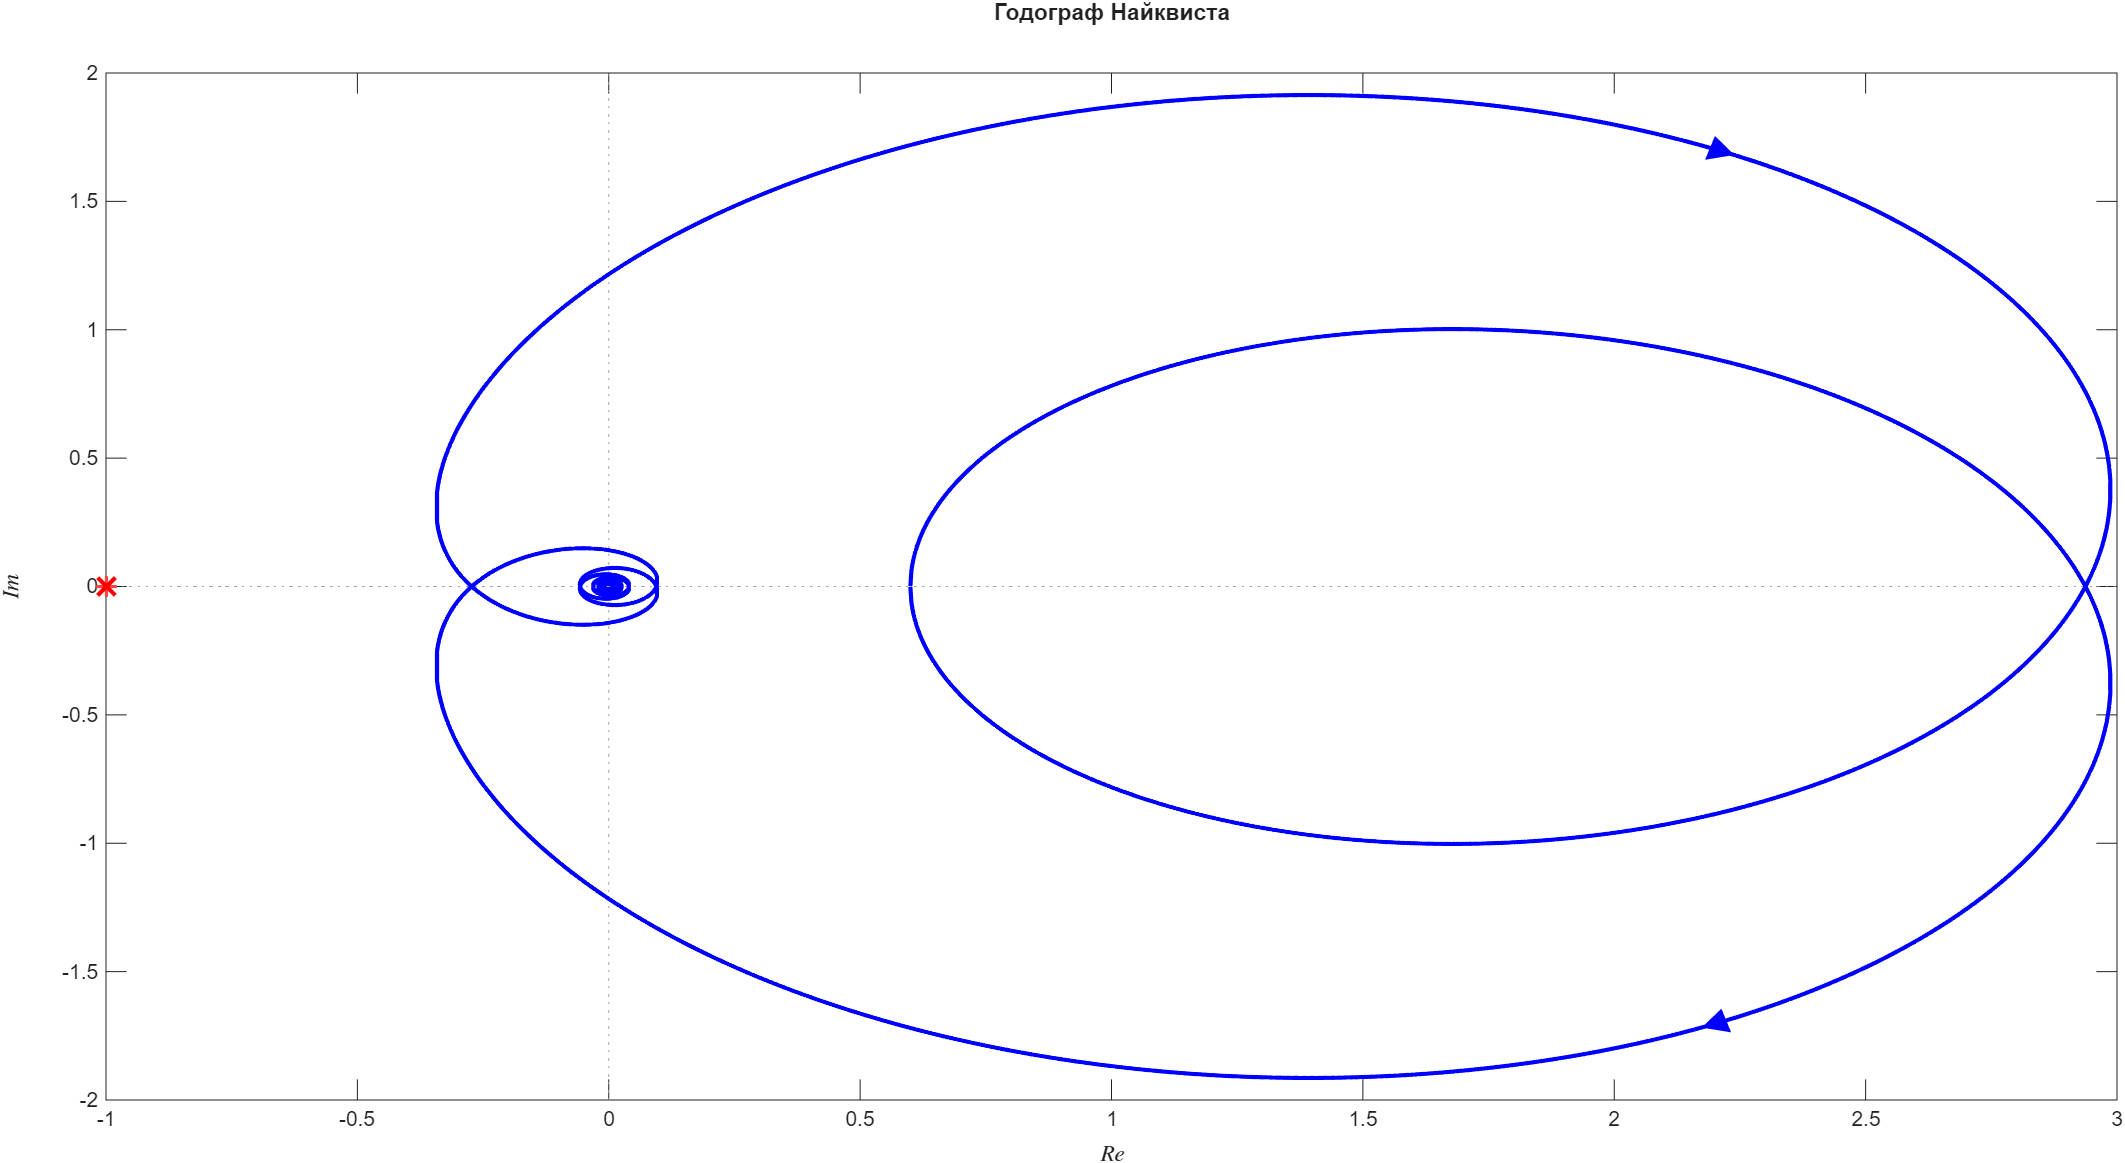
\includegraphics[width=0.75\linewidth]{images/Figure_6_3_1_4.png}
    \caption{Годограф Найквиста при $\tau = 0.05$ (3 передаточная функция)}
    \label{fig:placeholder}
\end{figure}

\begin{figure}[H]
    \centering
    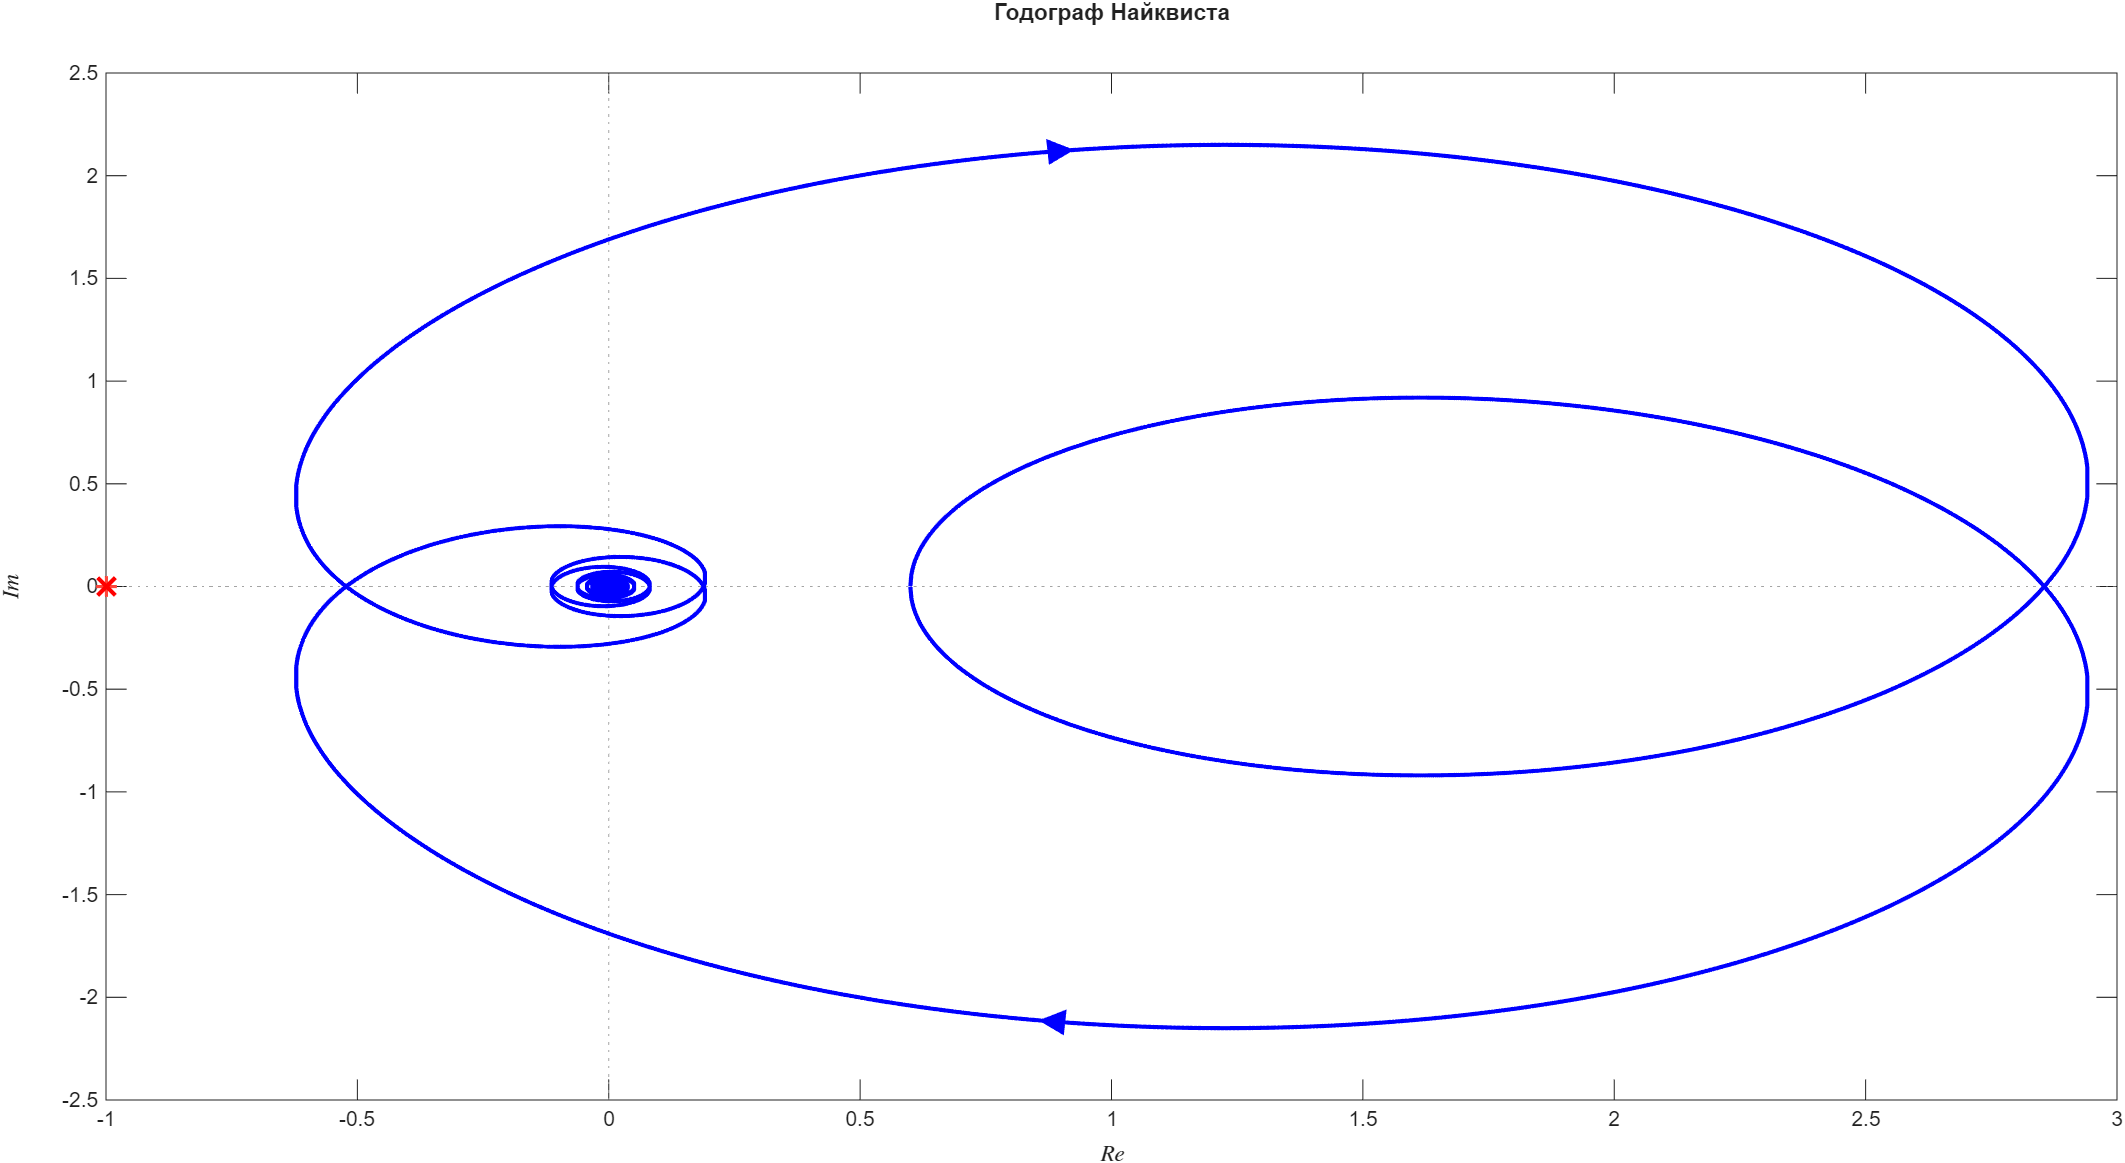
\includegraphics[width=0.75\linewidth]{images/Figure_6_3_1_5.png}
    \caption{Годограф Найквиста при $\tau = 0.1$ (3 передаточная функция)}
    \label{fig:placeholder}
\end{figure}

\begin{figure}[H]
    \centering
    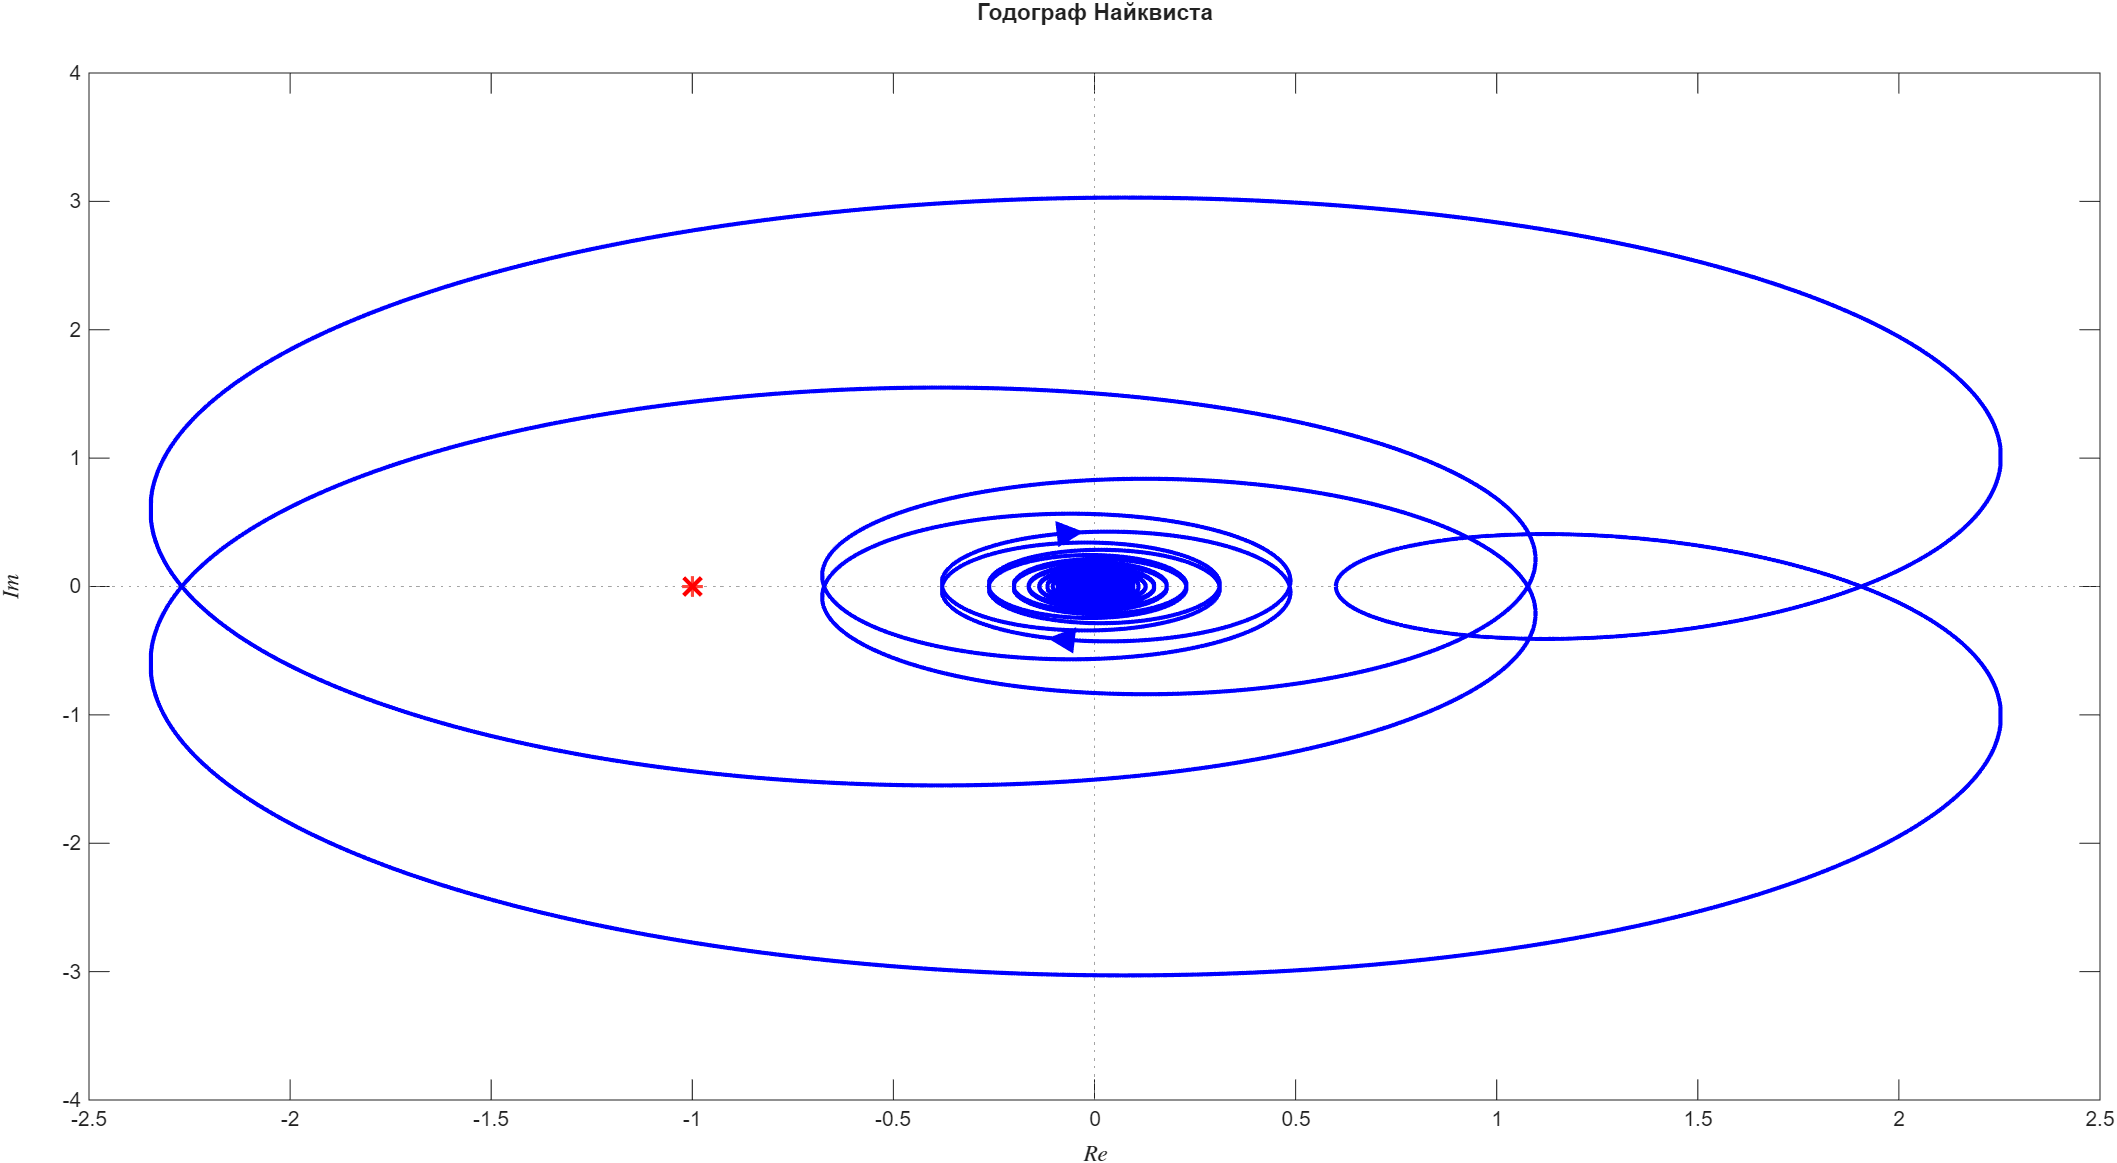
\includegraphics[width=0.75\linewidth]{images/Figure_6_3_1_6.png}
    \caption{Годограф Найквиста при $\tau = 0.6$ (3 передаточная функция)}
    \label{fig:placeholder}
\end{figure}

\begin{figure}[H]
    \centering
    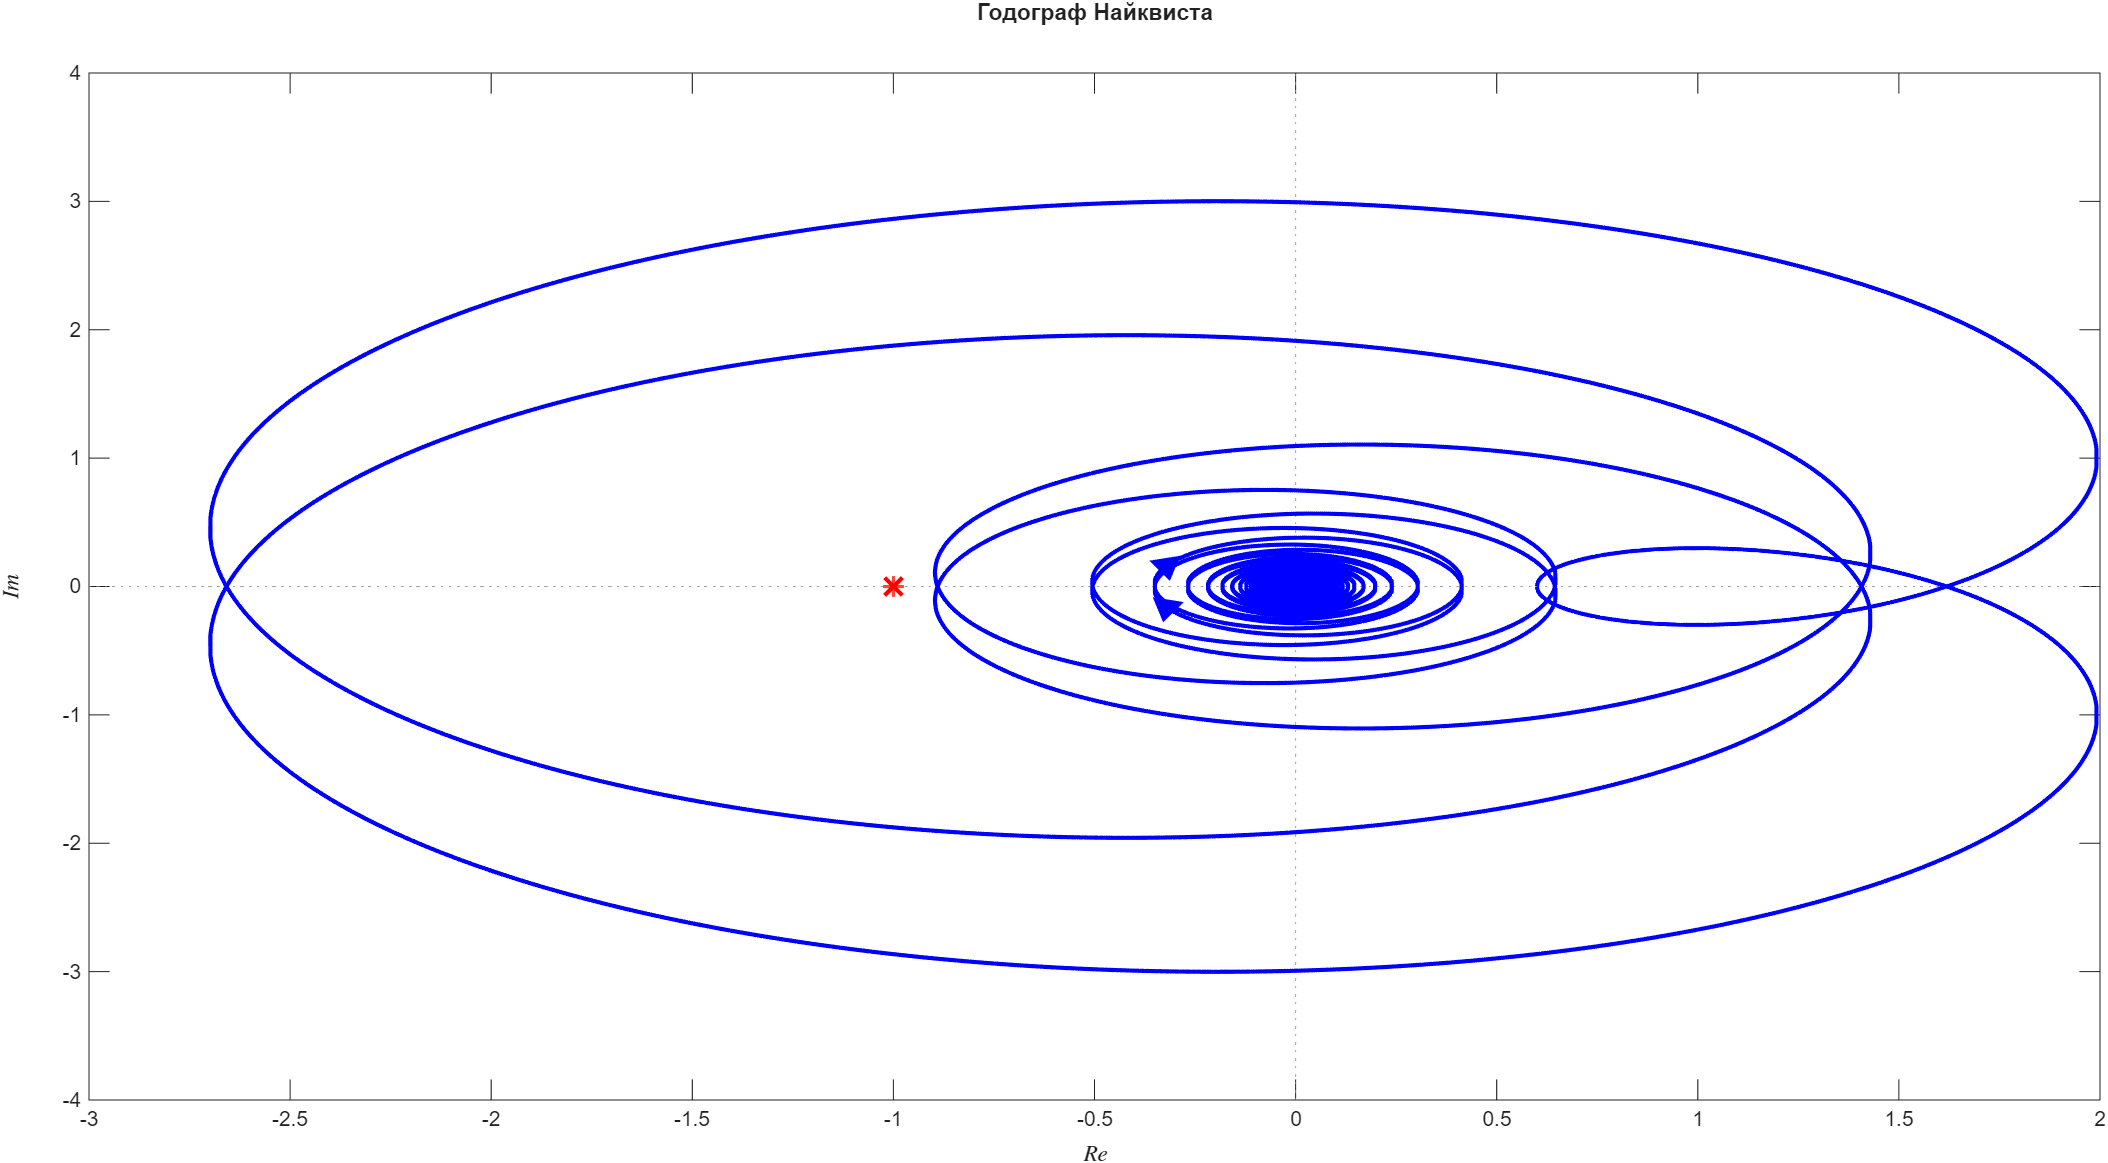
\includegraphics[width=0.75\linewidth]{images/Figure_6_3_1_7.png}
    \caption{Годограф Найквиста при $\tau = 0.8$ (3 передаточная функция)}
    \label{fig:placeholder}
\end{figure}

\begin{figure}[H]
    \centering
    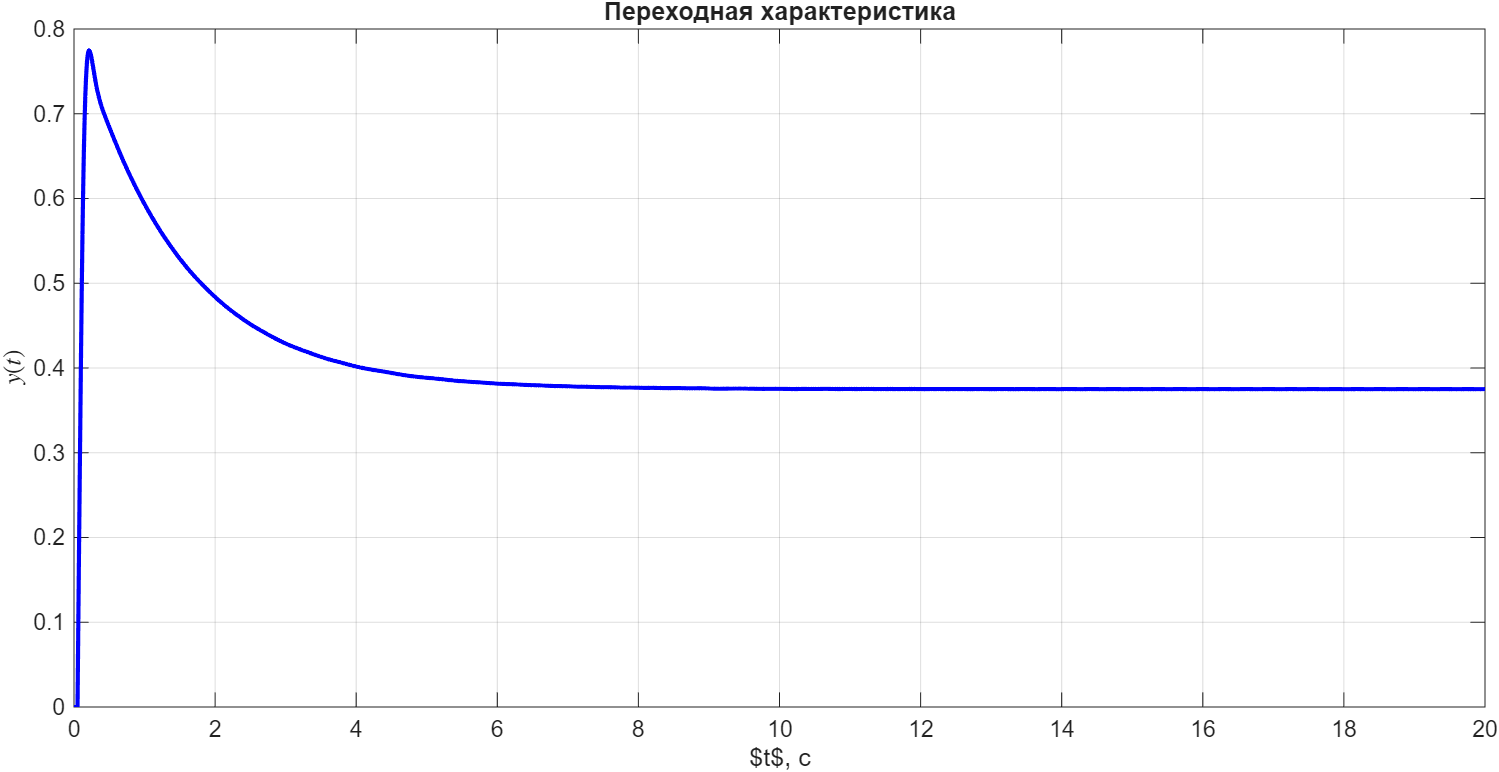
\includegraphics[width=0.75\linewidth]{images/Figure_6_3_1_8.png}
    \caption{Переходная характеристика при $\tau = 0.05$ (3 передаточная функция)}
    \label{fig:placeholder}
\end{figure}

\begin{figure}[H]
    \centering
    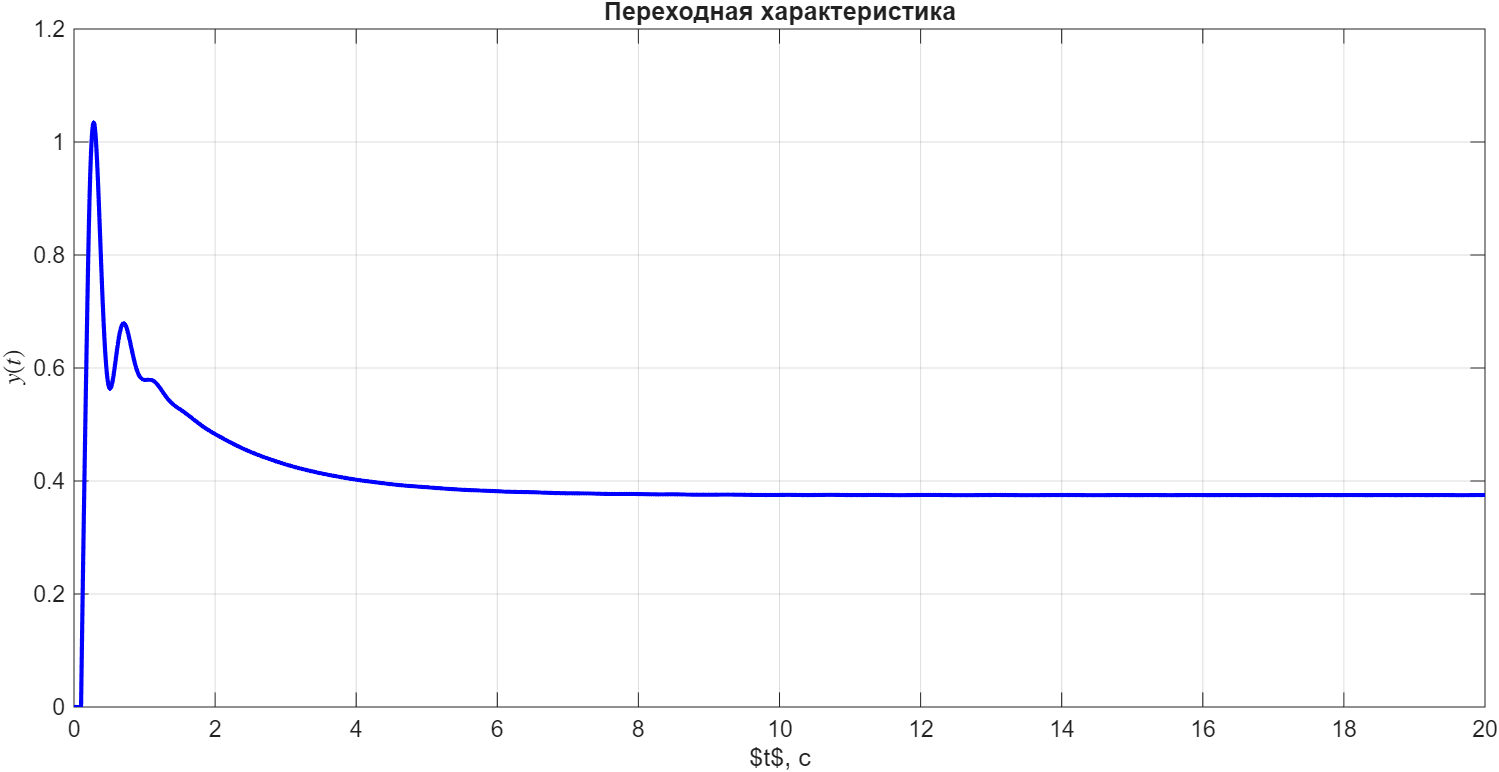
\includegraphics[width=0.75\linewidth]{images/Figure_6_3_1_9.png}
    \caption{Переходная характеристика при $\tau = 0.1$ (3 передаточная функция)}
    \label{fig:placeholder}
\end{figure}

\begin{figure}[H]
    \centering
    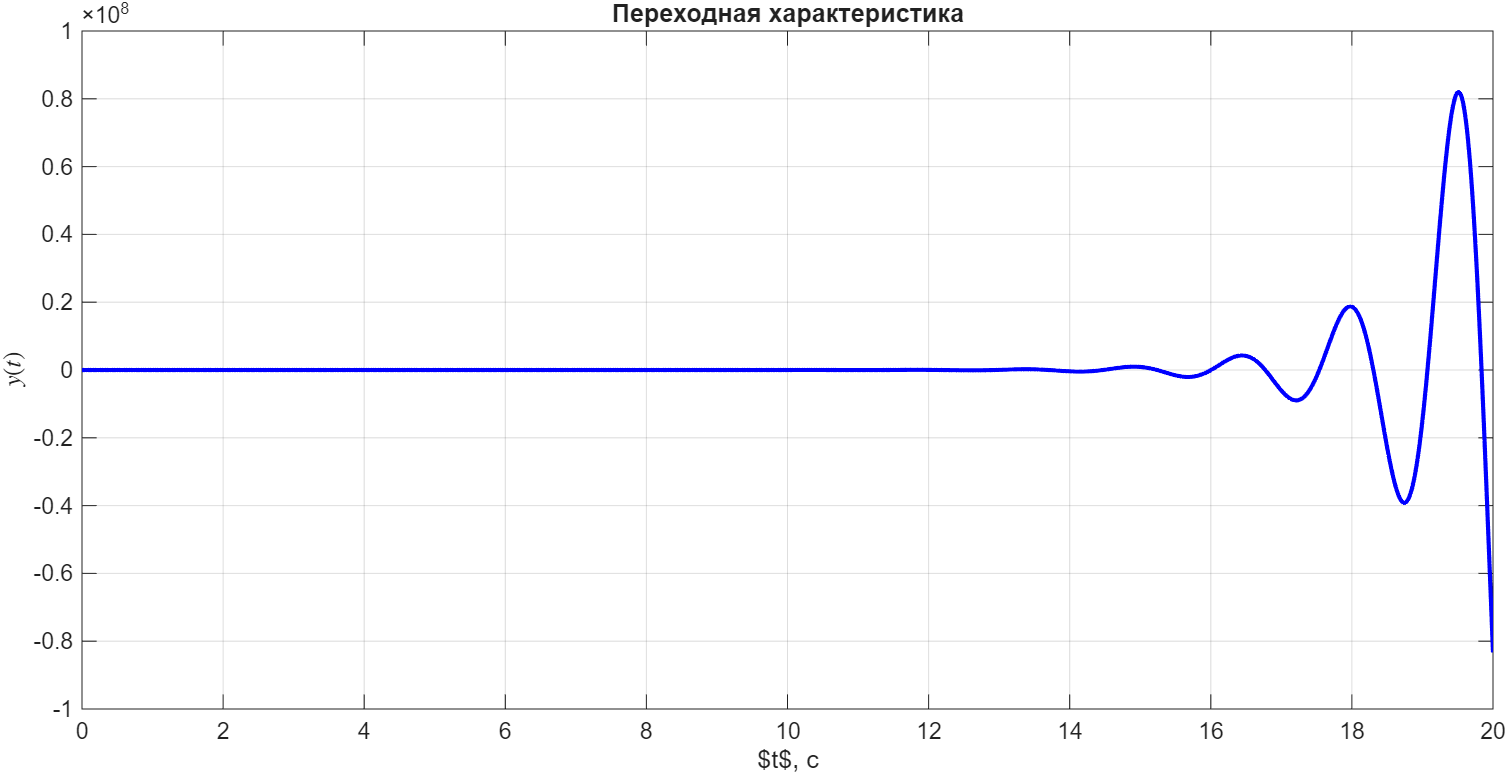
\includegraphics[width=0.75\linewidth]{images/Figure_6_3_1_10.png}
    \caption{Переходная характеристика при $\tau = 0.6$ (3 передаточная функция)}
    \label{fig:placeholder}
\end{figure}

\begin{figure}[H]
    \centering
    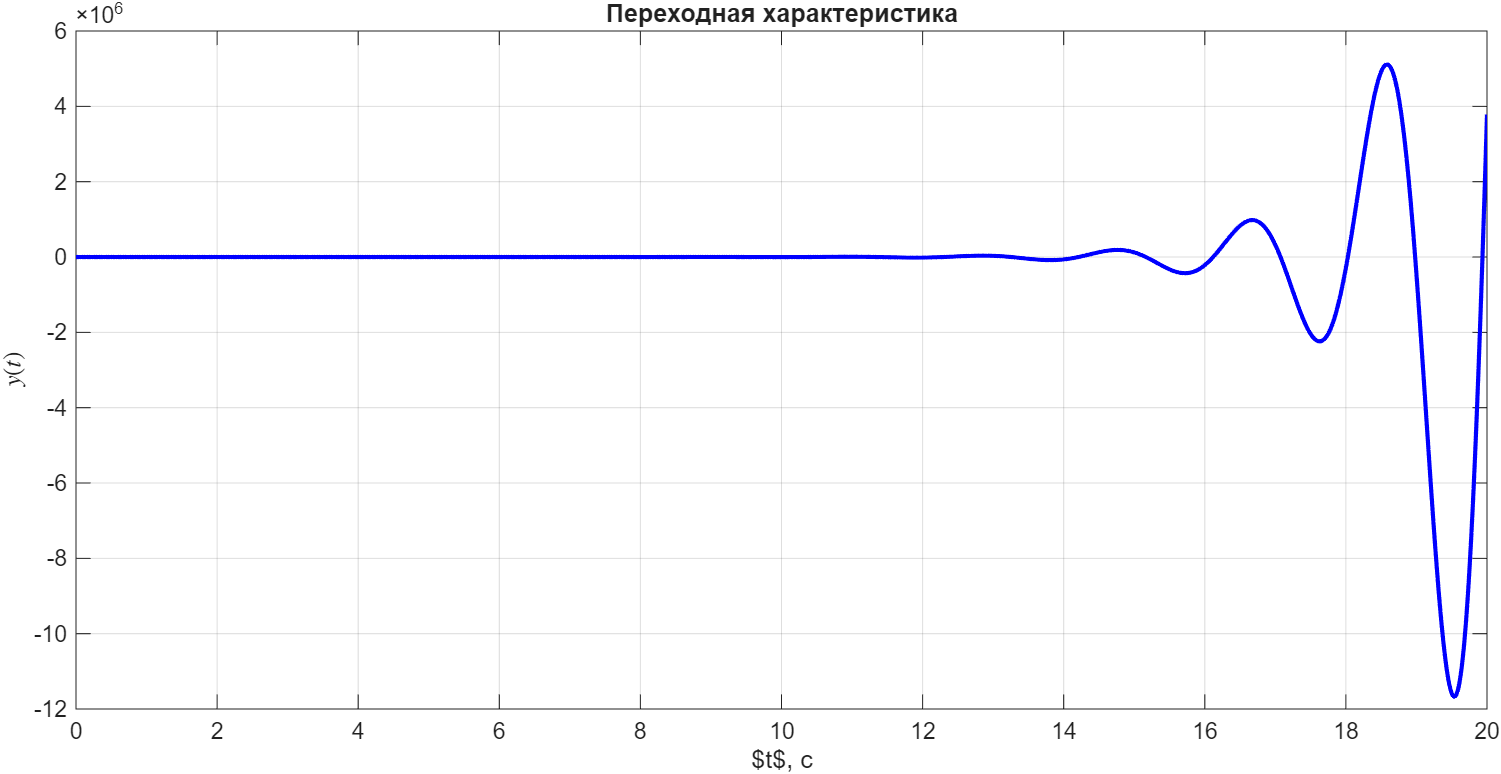
\includegraphics[width=0.75\linewidth]{images/Figure_6_3_1_11.png}
    \caption{Переходная характеристика при $\tau = 0.8$ (3 передаточная функция)}
    \label{fig:placeholder}
\end{figure}

Как мы видим на графиках, при $\tau>\tau_{\text{кр}}$ годограф Найквиста закручивается вокруг точки (-1, 0), из-за чего наблюдается потеря устойчивости, графики переходных характеристик соответствуют ожиданиям.




\subsection{Четвертая передаточная функция}

Добавим к передаточной функции звено чистого запаздывания:

$$
W(s)=e^{-\tau s}\dfrac{10s^2-6s+11}{10s^3-s^2+38s+20}
$$

Полюса разомкнутой системы:

\begin{figure}[H]
    \centering
    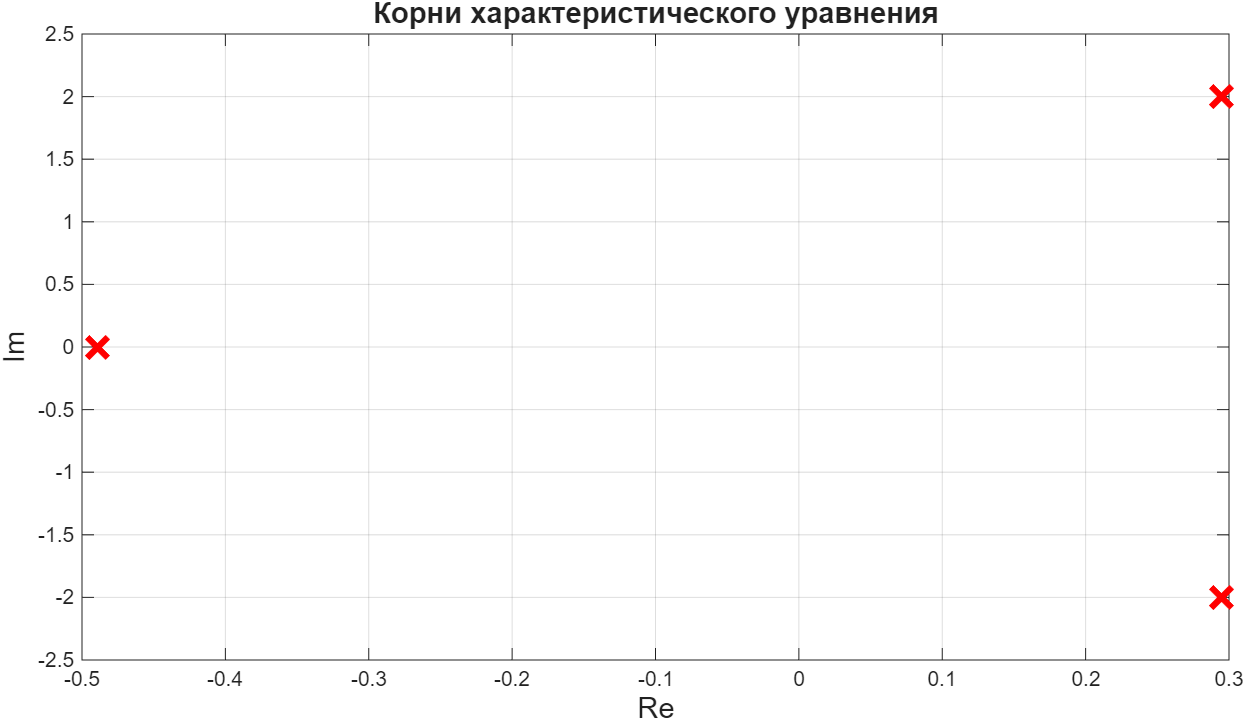
\includegraphics[width=0.75\linewidth]{images/Figure_6_3_2_1.png}
    \caption{Корни характеристического уравнения (4 передаточная функция)}
    \label{fig:placeholder}
\end{figure}

Разомкнутая система не устойчива

\begin{figure}[H]
    \centering
    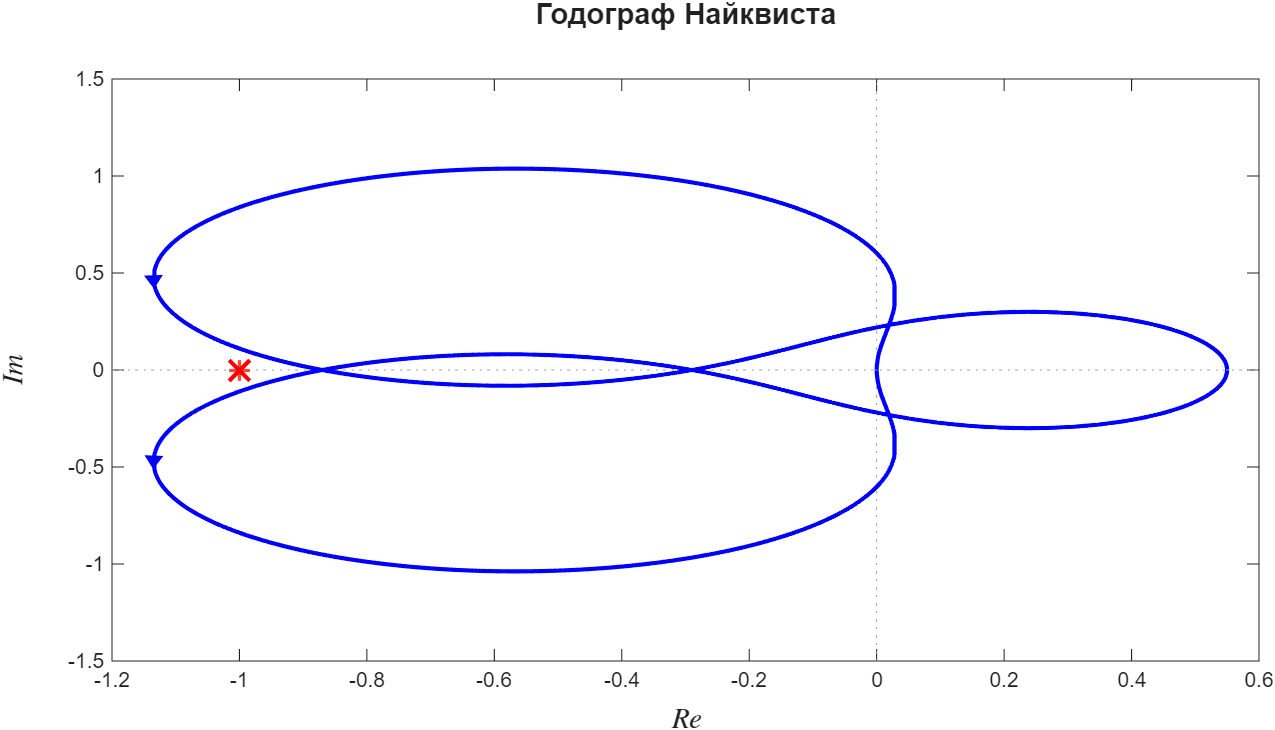
\includegraphics[width=0.75\linewidth]{images/Figure_6_3_2_2.png}
    \caption{Годограф Найквиста при $\tau = 0$ (4 передаточная функция)}
    \label{fig:placeholder}
\end{figure}

\begin{figure}[H]
    \centering
    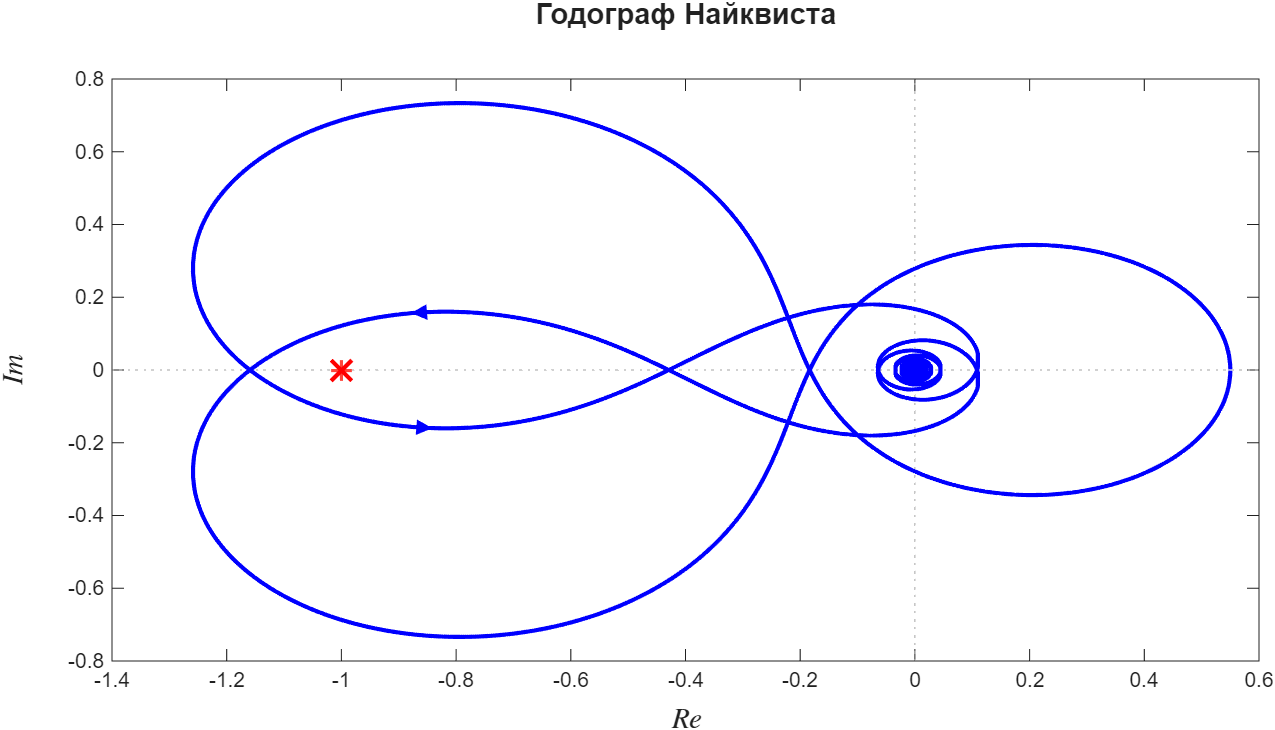
\includegraphics[width=0.75\linewidth]{images/Figure_6_3_2_3.png}
    \caption{Годограф Найквиста при $\tau = 0.5$ (4 передаточная функция)}
    \label{fig:placeholder}
\end{figure}

Частотная передаточная функция:

\[
W(j\omega) = \frac{10(j\omega)^2 - 6(j\omega) + 11}{10(j\omega)^3 - (j\omega)^2 + 38(j\omega) + 20}.
\]

Амплитуда:
\[
|W(j\omega)| = \sqrt{\frac{(-10\omega^2 + 11)^2 + (6\omega)^2}{(\omega^2 + 20)^2 + \bigl(\omega(38 - 10\omega^2)\bigr)^2}}.
\]

При \(|W(j\omega)| = 1\):
\[
(-10\omega_c^2 + 11)^2 + (6\omega_c)^2 = (\omega_c^2 + 20)^2 + \bigl(\omega_c(38 - 10\omega_c^2)\bigr)^2.
\]

Раскроем скобки:
\[
100\omega_c^6 - 859\omega_c^4 + 1668\omega_c^2 + 279 = 0.
\]

\[
\omega_{c1} \approx 2.33\ \text{рад/с}.
\]

\[
\omega_{c2} \approx 1.83\ \text{рад/с}.
\]

Фаза:
\[
\varphi_с(\omega) = \arg(11 - 10\omega^2 - 6j\omega) - \arg(20 + \omega^2 + j(38\omega - 10\omega^3))
\]

Для \(\omega_c = 2.33\):
\[
\varphi(j\omega_{c}) \approx -1.851 \text{ рад}
\]

Для \(\omega_c = 1.83\):
\[
\varphi(j\omega_{c}) \approx -3.027 \text{ рад} 
\]

Критические запаздывания:

Для \(\omega_c = 2.33\):
\[
\tau_{\text{кр.1}} = \dfrac{-1.851+\pi}{2.33}=0.554 
\]

Для \(\omega_c = 1.83\):
\[
\tau_{\text{кр.2}} = \dfrac{-3.027+\pi}{1.83}=0.063
\]

\[
\tau \in (0.063,\ 0.554)\ \text{с}.
\]

Возьмем $\tau =\{0.004,\ 0.2,\ 0.4,\ 2 \}$

Запас по фазе:

$\varphi_{\text{з}} = \pi + \varphi_0(\omega_{c1}) \approx 6.6^\circ$


\begin{figure}[H]
    \centering
    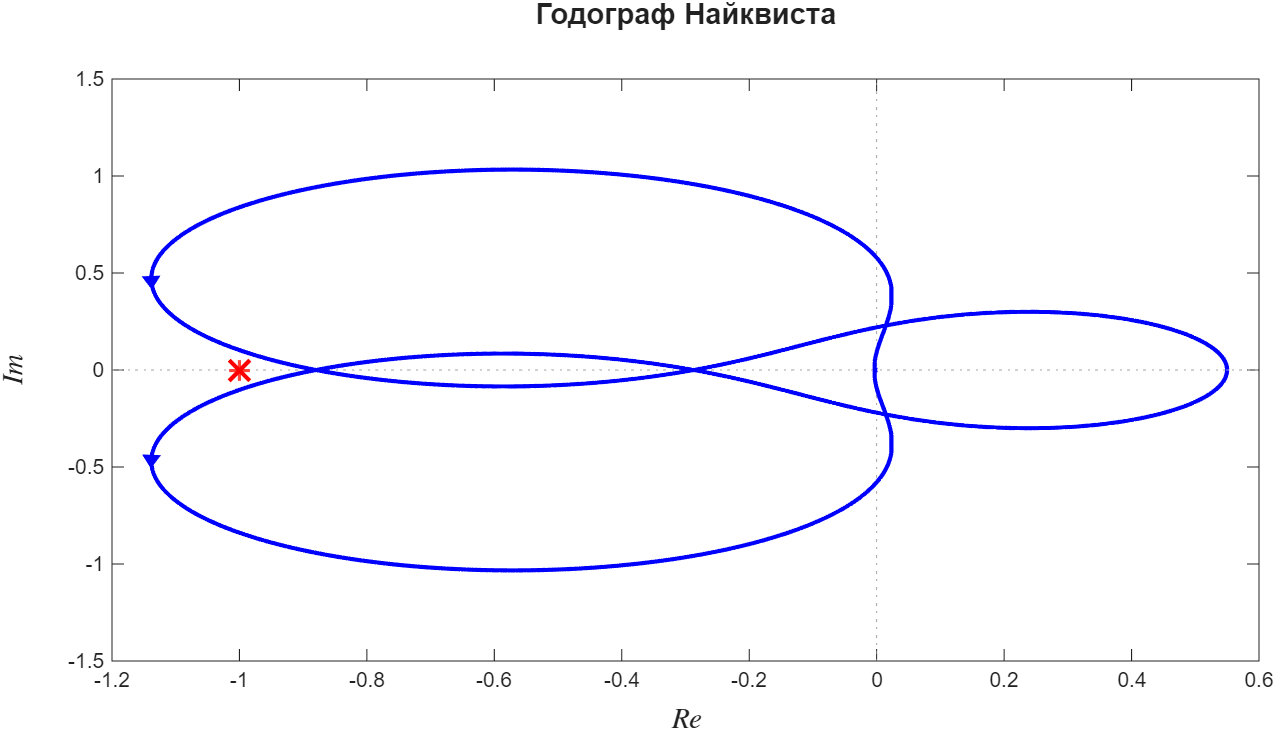
\includegraphics[width=0.75\linewidth]{images/Figure_6_3_2_4.png}
    \caption{Годограф Найквиста при $\tau = 0.2$ (4 передаточная функция)}
    \label{fig:placeholder}
\end{figure}

\begin{figure}[H]
    \centering
    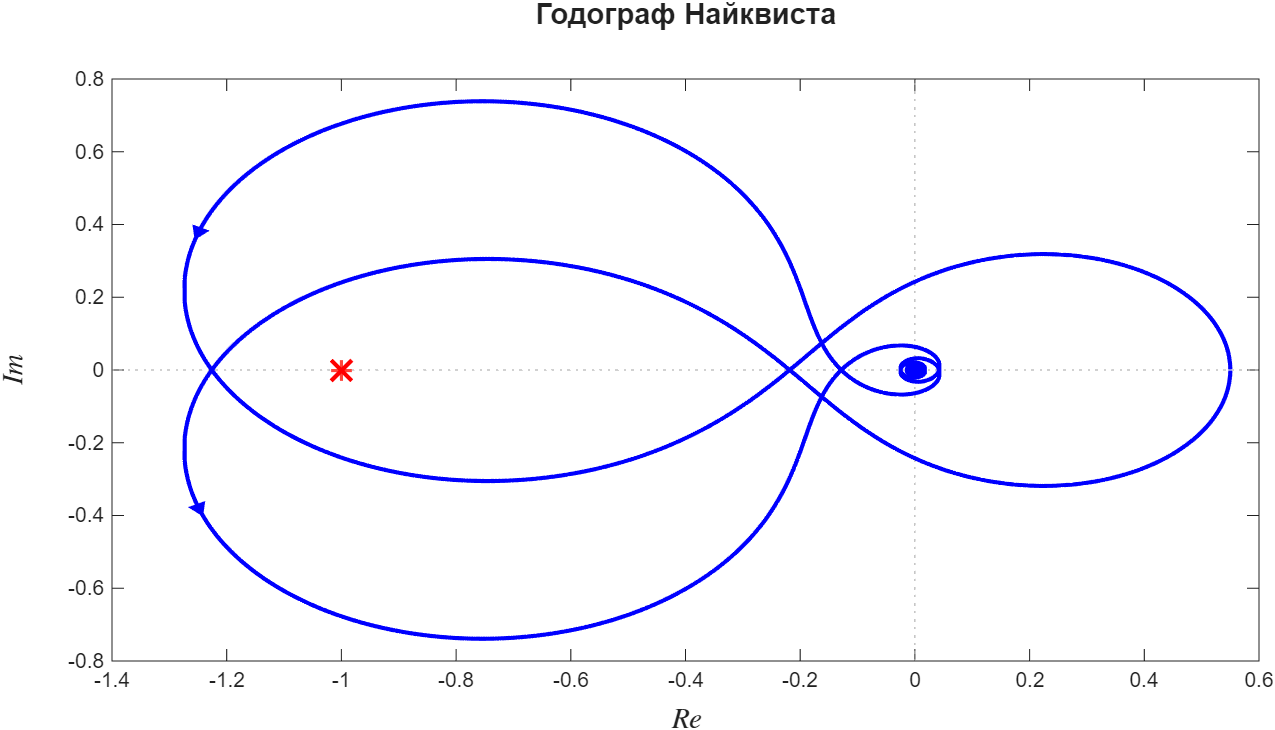
\includegraphics[width=0.75\linewidth]{images/Figure_6_3_2_5.png}
    \caption{Годограф Найквиста при $\tau = 1$ (4 передаточная функция)}
    \label{fig:placeholder}
\end{figure}

\begin{figure}[H]
    \centering
    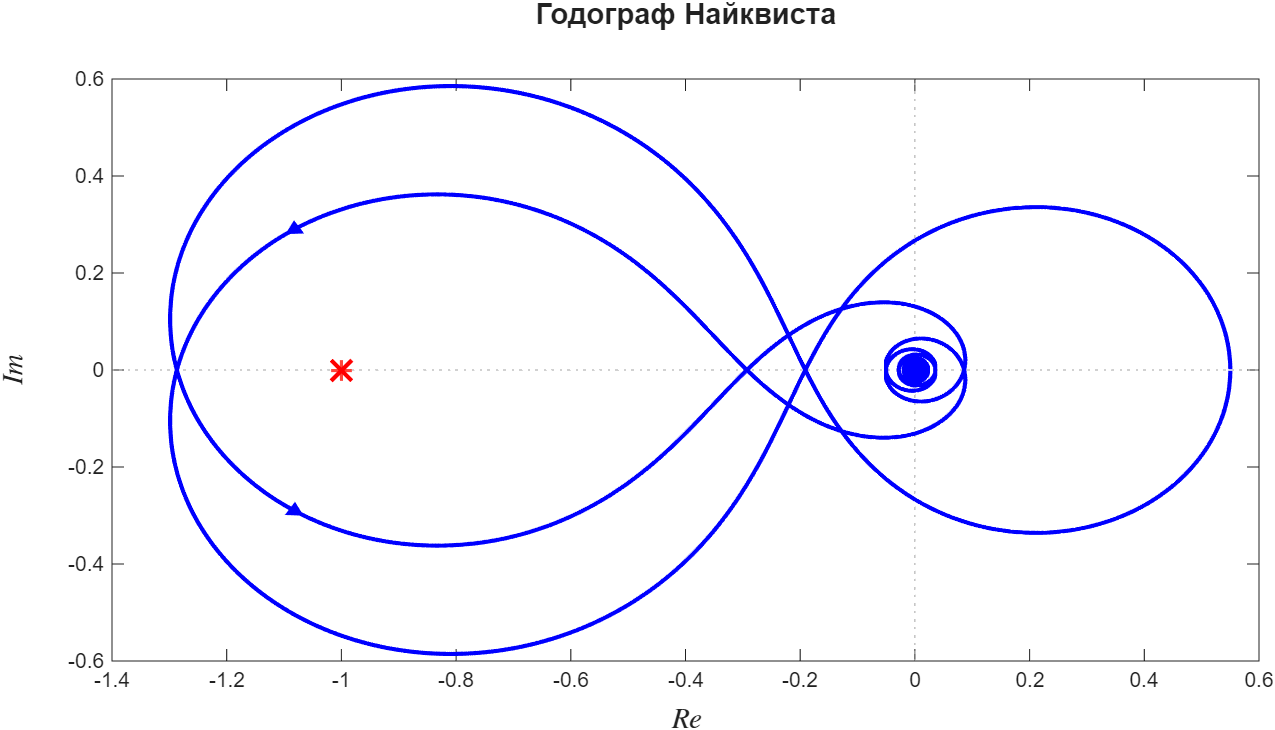
\includegraphics[width=0.75\linewidth]{images/Figure_6_3_2_6.png}
    \caption{Годограф Найквиста при $\tau = 2$ (4 передаточная функция)}
    \label{fig:placeholder}
\end{figure}

\begin{figure}[H]
    \centering
    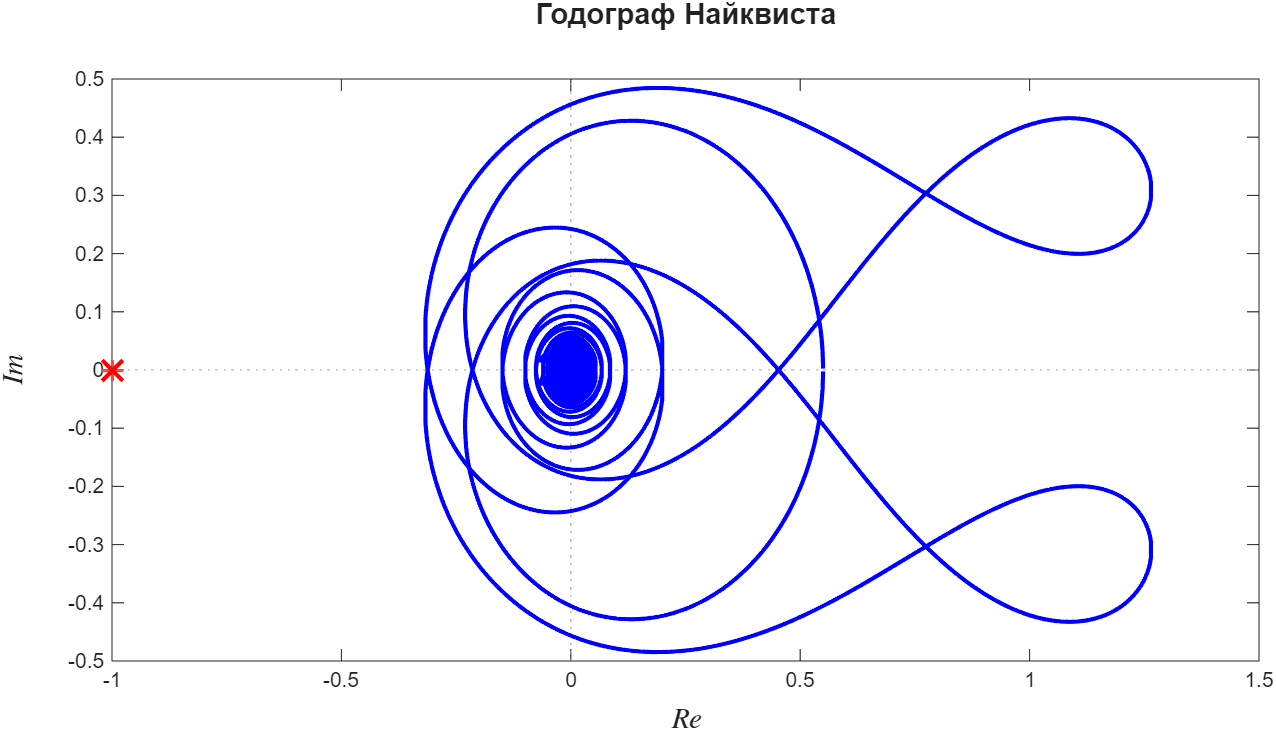
\includegraphics[width=0.75\linewidth]{images/Figure_6_3_2_7.png}
    \caption{Годограф Найквиста при $\tau = 6$ (4 передаточная функция)}
    \label{fig:placeholder}
\end{figure}

\begin{figure}[H]
    \centering
    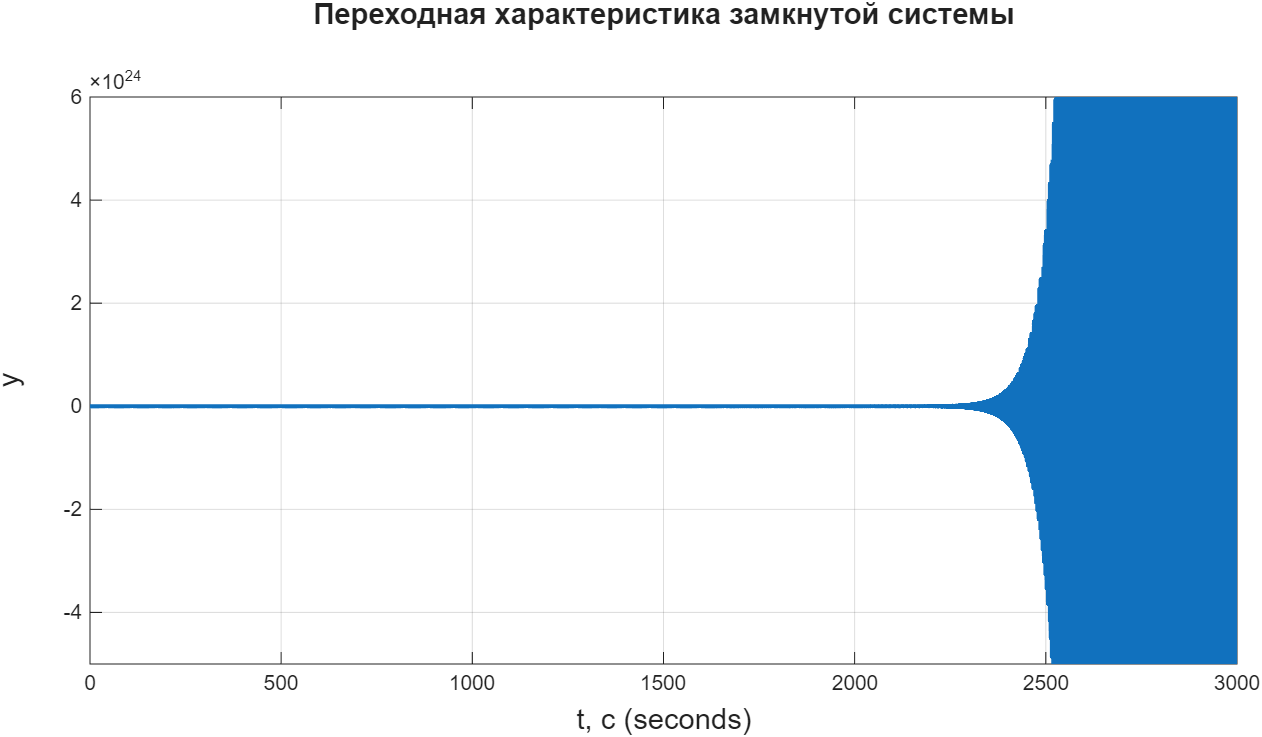
\includegraphics[width=0.75\linewidth]{images/Figure_6_3_2_8.png}
    \caption{Переходная характеристика при $\tau = 0.2$ (4 передаточная функция)}
    \label{fig:placeholder}
\end{figure}

\begin{figure}[H]
    \centering
    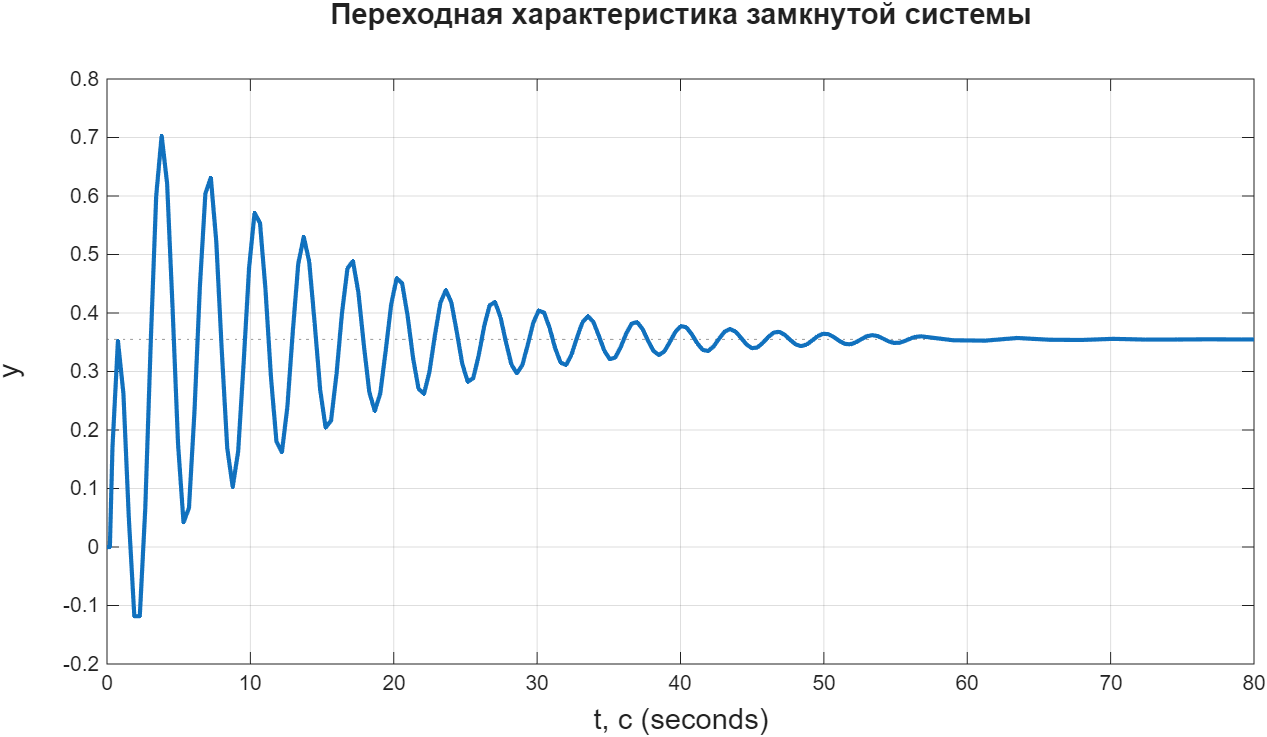
\includegraphics[width=0.75\linewidth]{images/Figure_6_3_2_9.png}
    \caption{Переходная характеристика при $\tau = 1$ (4 передаточная функция)}
    \label{fig:placeholder}
\end{figure}

\begin{figure}[H]
    \centering
    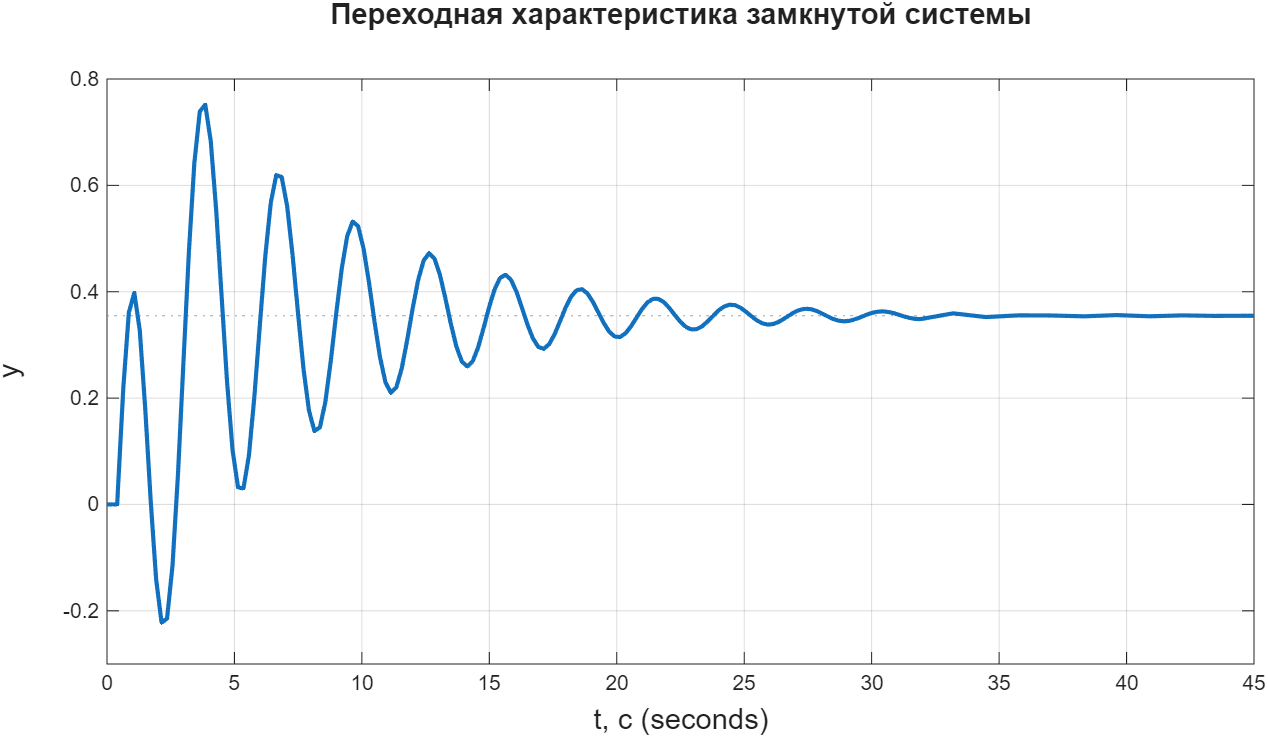
\includegraphics[width=0.75\linewidth]{images/Figure_6_3_2_10.png}
    \caption{Переходная характеристика при $\tau = 2$ (4 передаточная функция)}
    \label{fig:placeholder}
\end{figure}

\begin{figure}[H]
    \centering
    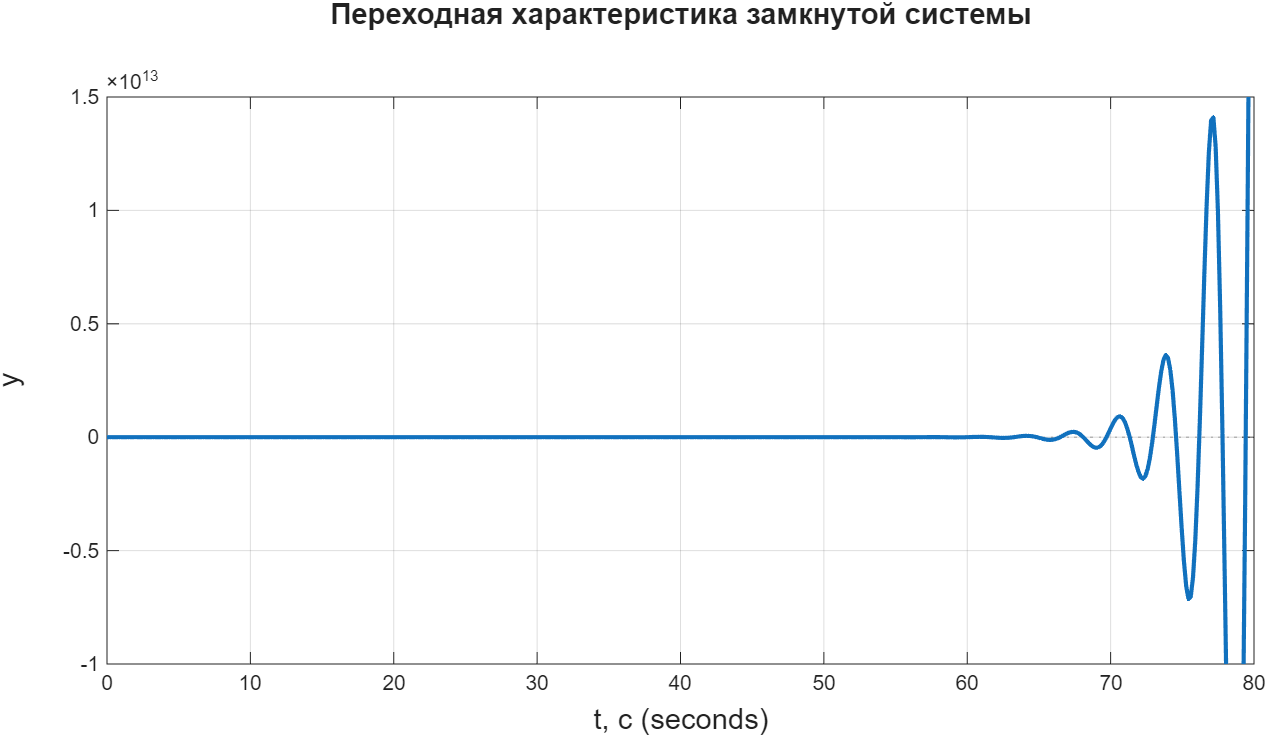
\includegraphics[width=0.75\linewidth]{images/Figure_6_3_2_11.png}
    \caption{Переходная характеристика при $\tau = 6$ (4 передаточная функция)}
    \label{fig:placeholder}
\end{figure}

Как мы видим на графиках, при значениях $\tau$ не из найденного нами промежутка годограф Найквиста не делает нужного числа оборотов вокруг точки (-1, 0) по часовой стрелке, из-за чего наблюдается потеря устойчивости, графики переходных характеристик соответствуют ожиданиям.


\section{Выводы}

В ходе выполнения данной практической работы были изучены и применены на практике критерии устойчивости Найквиста для анализа линейных систем.

Для трёх объектов с заданным количеством неустойчивых полюсов в разомкнутом и замкнутом состоянии были составлены передаточные функции, удовлетворяющие условиям варианта. Для каждого объекта было проведено моделирование и получены карты нулей и полюсов, переходные характеристики, а также годографы Найквиста. Выполнена проверка устойчивости замкнутых систем по критерию Найквиста: подсчитано количество оборотов годографа вокруг критической точки \((-1, 0)\) и подтверждено выполнение условия \( N = m - n \). Теоретические расчёты совпали с результатами моделирования, что подтвердило корректность построенных моделей.

Также был освоен логарифмический критерий Найквиста. Для каждой системы были построены ЛАЧХ и ЛФЧХ, определено количество переходов ЛФЧХ через критические уровни в области положительной ЛАЧХ, и сделан вывод об устойчивости. Результаты логарифмического критерия полностью согласовались с классическим критерием Найквиста.

Во втором задании было исследовано влияние коэффициента усиления \(k\) на устойчивость замкнутой системы. Для двух передаточных функций были построены годографы при различных \(k\), аналитически найдены границы устойчивости и проанализирована зависимость количества неустойчивых полюсов от \(k\). 

В третьем задании исследовано влияние звена чистого запаздывания \(e^{-\tau s}\) на устойчивость системы. Для двух передаточных функций были рассчитаны критические значения запаздывания \(\tau_{\text{кр}}\) при помощи анализа АФЧХ. Построены годографы Найквиста и переходные характеристики для значений \(\tau\) как меньше, так и больше критического. 

Таким образом, в ходе работы были закреплены навыки анализа устойчивости систем как по классическому, так и по логарифмическому критерию Найквиста, а также исследовано влияние параметров системы (коэффициента усиления и времени запаздывания) на её устойчивость. Полученные практические результаты полностью соответствуют теоретическим положениям.

\end{document}